\documentclass[]{book}
\usepackage{url,amsfonts, amsmath, amssymb, amsthm,color, enumerate, multicol, systeme, amsthm, varwidth, cancel}
\usepackage[framemethod=TikZ]{mdframed}
\usepackage[export]{adjustbox}
\usepackage{graphicx}
\usepackage[utf8]{inputenc}
\usepackage[margin=1.0in]{geometry}
\usepackage{hyperref}
\usepackage{thmtools}
\usepackage{tikz}
\usepackage{yfonts}
\usepackage{float}
\usepackage{wrapfig}
\usepackage{tikz-cd}
\newcommand{\listoftheoremname}{List of theorems and definitions}

\makeatletter

\DeclareMathOperator{\rref}{rref}
\renewcommand*\env@matrix[1][*\c@MaxMatrixCols c]{%
  \hskip -\arraycolsep
  \let\@ifnextchar\new@ifnextchar
  \array{#1}}
\makeatother
\allowdisplaybreaks
\DeclareMathOperator{\vecspan}{span}
\DeclareMathOperator{\spacedim}{dim}
\DeclareMathOperator{\rank}{rank}
\DeclareMathOperator{\proj}{proj}
\DeclareMathOperator{\vecref}{ref}
\DeclareMathOperator{\image}{Im}
\DeclareMathOperator{\preimage}{PreIm}
\DeclareMathOperator{\kernel}{Ker}
\DeclareMathOperator{\rotation}{Rot}
\newcommand{\inv}[1]{\ensuremath{{#1}^{-1}}}
\newcommand{\invm}[1]{\ensuremath{\inv{\mat{#1}}}}
\newcommand*{\vvec}[1]{\overrightarrow{#1}}
\newcommand{\bas}[1]{\ensuremath{\mathfrak{#1}}}
\newcommand{\coordb}[2]{\ensuremath{\left[#1\right]_{#2}}}
\newcommand{\nextline}{\hspace*{0pt}\newline}

\newcount\colveccount
\newcommand*\colvec[1]{
        \global\colveccount#1
        \begin{bmatrix}
        \colvecnext
}
\def\colvecnext#1{
        #1
        \global\advance\colveccount-1
        \ifnum\colveccount>0
                \\
                \expandafter\colvecnext
        \else
                \end{bmatrix}
        \fi
}
\newcommand{\vecxx}[1][x]{\ensuremath{\begin{bmatrix}
#1_1 \\
#1_2
\end{bmatrix}}}
\newcommand{\vecxxx}[1][x]{\ensuremath{\begin{bmatrix}
#1_1 \\
#1_2 \\
#1_3
\end{bmatrix}}}
\newcommand{\vecxxxx}[1][x]{\ensuremath{\begin{bmatrix}
#1_1 \\
#1_2 \\
#1_3 \\
#1_4
\end{bmatrix}}}
\newcommand{\vecxxdx}[1][x]{\ensuremath{\begin{bmatrix}
#1_1 \\
#1_2 \\
\vdots \\
#1_n
\end{bmatrix}}}
\newcommand{\vecn}[1]{\ensuremath{\vec{v}_{#1}}}
\newcommand{\sbvec}[1]{\ensuremath{\vec{e}_#1}}
\newcommand{\vecxy}{\ensuremath{\colvec{2}{x}{y}}}

\newcommand{\suchthat}{\,\middle|\,}
\newcommand{\mat}[1]{\ensuremath{\mathbf{#1}}}
\newcommand{\cmat}[1][v]{\begin{bmatrix}
        \vert & \vert & & \vert \\
        \vec{#1}_1 & \vec{#1}_2 & \cdots & \vec{#1}_n \\
        \vert & \vert & & \vert
    \end{bmatrix}
}
\newcommand{\idmat}[1][n]{\ensuremath{\mat{I}_#1}}

\newcommand{\imat}{\ensuremath{\begin{bmatrix}
1 & 0 & \cdots & 0 \\
0 & 1 & \cdots & 0 \\
\vdots & \vdots & \ddots & \vdots \\
0 & 0 & \cdots & 1\end{bmatrix}}}

\newcommand{\R}{\ensuremath{\mathbb{R}}}
\newcommand{\Rn}{\ensuremath{\R^n}}
\newcommand{\Rm}{\ensuremath{\R^m}}

\newcommand{\elemmatnn}[1][a]{\ensuremath{\begin{bmatrix}
{#1}_{11} & {#1}_{12} & \cdots & {#1}_{1n} \\
{#1}_{21} & {#1}_{22} & \cdots & {#1}_{2n} \\
\vdots    & \vdots    & \ddots & \vdots    \\
{#1}_{n1} & {#1}_{n2} & \cdots & {#1}_{nn}
\end{bmatrix}}}

\newcommand{\elemmatmn}[1][a]{\ensuremath{\begin{bmatrix}
{#1}_{11} & {#1}_{12} & \cdots & {#1}_{1n} \\
{#1}_{21} & {#1}_{22} & \cdots & {#1}_{2n} \\
\vdots    & \vdots    & \ddots & \vdots    \\
{#1}_{m1} & {#1}_{m2} & \cdots & {#1}_{mn}
\end{bmatrix}}}


\newmdtheoremenv{theorem}{Theorem}[section]
\newmdtheoremenv{corollary}{Corollary}[section]
\newmdtheoremenv{example}{Example}[section]
\newtheorem*{solution}{Solution}
\newtheorem*{intuition}{Intuition}
\newtheorem*{remark}{Remark}
\newmdtheoremenv{definition}{Definition}[section]

\title{Linear Algebra Notes}
\author{Yiliang Liang, uniqname \texttt{yiliangl} }

\date{}

\begin{document}

\begin{titlepage} % Suppresses headers and footers on the title page
	\centering % Centre everything on the title page
	\scshape % Use small caps for all text on the title page
	
	\vspace*{5cm} % White space at the top of the page
	
	%------------------------------------------------
	%	Title
	%------------------------------------------------
	
	\rule{\textwidth}{1.6pt}\vspace*{-\baselineskip}\vspace*{2pt} % Thick horizontal rule
	\rule{\textwidth}{0.4pt} % Thin horizontal rule
	
	\vspace{0.75\baselineskip} % Whitespace above the title
	
	{\LARGE LINEAR ALGEBRA\\ Notes\\} % Title
	
	\vspace{0.75\baselineskip} % Whitespace below the title
	
	\rule{\textwidth}{0.4pt}\vspace*{-\baselineskip}\vspace{3.2pt} % Thin horizontal rule
	\rule{\textwidth}{1.6pt} % Thick horizontal rule
	
	\vspace{2\baselineskip} % Whitespace after the title block
	
	%------------------------------------------------
	%	Subtitle
	%------------------------------------------------
	
	A Compilation of Notes \\ From Khan Academy's Linear Algebra Course \\ And MATH 214% Subtitle or further description
	
	\vspace*{3\baselineskip} % Whitespace under the subtitle
	
	%------------------------------------------------
	%	Editor(s)
	%------------------------------------------------
	
	Written and Edited By
	
	\vspace{0.5\baselineskip} % Whitespace before the editors
	
	{\scshape\Large \textgoth{Yiliang ``Leo'' Liang} \\
	\small Uniqname: \texttt{YILIANGL}} % Editor list
	
	\vspace{0.5\baselineskip} % Whitespace below the editor list
	
	\textit{\textfrak{University of Michigan, Ann Arbor}} % Editor affiliation
\end{titlepage}


\tableofcontents
\renewcommand{\listtheoremname}{List of Theorems}
\listoftheorems[ignoreall,show={theorem}]

\renewcommand{\listtheoremname}{List of Definitions}
\listoftheorems[ignoreall,show={definition}]
\chapter{Spaces and Basis}

\section{Linear Combinations and Span}
Let $\vec{v}_1,\vec{v}_2,\cdots,\vec{v}_n \in \mathbb{R}^n$ be vectors. Let
\[\vec{x} = c_1\vec{v}_1 + c_2\vec{v}_2 + \cdots + c_n\vec{v}_n\] for $c_n \in \mathbb{R}$.
\begin{definition}[linear combination]
    $\vec{x}$ is a \textbf{linear combination} of $\vec{v}_1,\vec{v}_2,\cdots,\vec{v}_n$.
\end{definition}
\begin{definition}[span] We define \textbf{span} as follows: 
    \[\vecspan(\vec{v}_1, \vec{v}_2, \cdots, \vec{v}_n) = \left\{c_1\vec{v}_1 + c_2\vec{v}_2 + \cdots + c_n\vec{v}_n \suchthat c_i \in \mathbb{R} \text{ for } 1 \leq i \leq n \right\}.\]

    Essentially, span of some vectors is the set of all linear combinations of the vectors.
\end{definition}

\section{Linear Dependence and Linear Independence}

\begin{definition}[linear dependence and independence]Let $S = \{\vec{v}_1, \vec{v}_2, \cdots, \vec{v}_n\}$. $S$ is \textbf{linearly independent} if no vectors in $S$ is the linear combination of some other vectors in $S$. On the other hand, $S$ is \textbf{linear dependent} if there exists $\vec{v} \in S$ such that $\vec{v}$ is the linear combination of $S \setminus \{\vec{v}\}$.
\end{definition}
\begin{theorem}[Property of Linear Dependence]
    \label{thm:linear_dependent}
    Let $S = \{\vec{v}_1, \vec{v}_2, \cdots, \vec{v}_n\}$. $S$ is linearly dependent if and only if $c_1\vec{v}_1 + \cdots + c_n\vec{v}_n = \vec{0}$ for some $c_i$'s such that at least one $c_i$ is non-zero.
\begin{proof}
    Suppose $S$ is linearly dependent. Then, by definition, there exists some $\vec{v}_1 \in S$ such that
    \[\vec{v}_1 = a_2\vec{v}_2 + a_3\vec{v}_3 + \cdots + a_n\vec{v}_n\]
    for $a_i \in \mathbb{R}$, where $\vec{v}_2, \vec{v}_3, \cdots, \vec{v}_n \neq \vec{v}_1$ and $\vec{v}_2, \vec{v}_3, \cdots, \vec{v}_n \in S$.
    Subtracting $\vec{v}_1$ from both sides, we have
    \[\vec{0} = -1\vec{v}_1 + a_2\vec{v}_2 + a_3\vec{v}_3 + \cdots + a_n\vec{v}_n.\]
    
    Now suppose $c_1\vec{v}_1 + \cdots + c_n\vec{v}_n = \vec{0}$ for some $c_i$'s such that at least one $c_i$ is non-zero. Without loss of generality, assume $c_1 \neq 0$. Then, we divide both sides by $c_1$ to yield
    \begin{align*}
        \vec{v}_1 + \frac{c_2}{c_1} \vec{v}_2 + \cdots + \frac{c_n}{c_1}\vec{v}_n &= \vec{0} \\
        \vec{v}_1 &= -\frac{c_2}{c_1}\vec{v}_2 - \cdots - \frac{c_n}{c_1}\vec{v}_n.
    \end{align*}
\end{proof}
\end{theorem}


\begin{example}
    Are $\vec{v}_1 = \begin{bmatrix}2 \\ 1\end{bmatrix}$ and $\vec{v}_2 = \begin{bmatrix}3 \\ 2\end{bmatrix}$ linearly independent?
\begin{solution}
    Consider equation
    \[c_1 \begin{bmatrix}2 \\ 1\end{bmatrix} + c_2 \begin{bmatrix}3 \\ 2\end{bmatrix} = \vec{0}.\]
    
    According to Theorem \ref{thm:linear_dependent}, $\vec{v}_1$ and $\vec{v}_2$ are linearly dependent if $c_1$ or $c_2$ are nonzero, and are linearly independent if both $c_1$ and $c_2$ are zero. We want to solve
    \begin{align*}
        2c_1 + 3c_2 &= 0 \\
        c_1 + 2c_2 &= 0
    \end{align*}
    Solving the equation, we have $c_1=c_2=0$ which means the vectors are linearly independent. \hfill\qedsymbol
\end{solution}
\end{example}

\begin{example}
    Are $\vec{v}_1 = \begin{bmatrix}2 \\ 1\end{bmatrix}$, $\vec{v}_2 = \begin{bmatrix}3 \\ 2\end{bmatrix}$, and $\vec{v}_3 = \begin{bmatrix}1 \\ 2\end{bmatrix}$ linearly independent or linearly dependent?
\begin{solution}
    We want to solve equation \[c_1\begin{bmatrix}2 \\ 1\end{bmatrix} + c_2\begin{bmatrix}3 \\ 2\end{bmatrix} + c_3\begin{bmatrix}1 \\ 2\end{bmatrix} = \vec{0}.\]
    
    There are infinitely many solutions. Pick $c_3=-1$. Then, $c_2=3$ and $c_1=-4$. Since there exists nonzero solutions, the vectors are linearly dependent. \hfill\qedsymbol
\end{solution}
\end{example}
\begin{example}
    Let $S=\left\{\begin{bmatrix}1 \\ -1 \\ 2\end{bmatrix}, \begin{bmatrix}2\\ 1 \\ 3\end{bmatrix}, \begin{bmatrix}-1 \\ 0 \\ 2\end{bmatrix}\right\}$. Is it true that $\vecspan(S)=\mathbb{R}^3$? Is $S$ linearly independent?
\begin{solution}
    Pick any vectors $\vec{v} = \begin{bmatrix}a\\ b \\ c\end{bmatrix} \in \mathbb{R}^3$. We want to show that there exists $c_1,c_2,c_3$ such that 
    \[c_1\begin{bmatrix}1 \\ -1 \\ 2\end{bmatrix} + c_2\begin{bmatrix}2\\ 1 \\ 3\end{bmatrix} + c_3\begin{bmatrix}-1 \\ 0 \\ 2\end{bmatrix} = \begin{bmatrix}a\\ b \\ c\end{bmatrix}.\]
    
    Solving this equation yields $c_3 = \frac{1}{11}(3c-5a+b)$, $c_2 = \frac{1}{3}(b+a+c_3)$, and $c_1 = a - 2c_2 + c_3$. Since any vectors in $\mathbb{R}^3$ can be represented by some linear combinations of $S$, $\vecspan(S) = \mathbb{R}^3$.
    
    $S$ is linearly independent if the only solutions to equation
    \[c_1\begin{bmatrix}1 \\ -1 \\ 2\end{bmatrix} + c_2\begin{bmatrix}2\\ 1 \\ 3\end{bmatrix} + c_3\begin{bmatrix}-1 \\ 0 \\ 2\end{bmatrix} = \begin{bmatrix}0\\ 0 \\ 0\end{bmatrix}\] is $(c_1,c_2,c_3)=(0,0,0)$. This is exactly the case when $\vec{v}=\vec{0}$, i.e. $a=b=c=0$. Then, $c_1=c_2=c_3=0$ by plugging into the solutions above. Hence $S$ is linearly independent. \hfill\qedsymbol
\end{solution}
\end{example}


\section{Linear Subspaces}
\begin{definition}[linear subspaces]
Let $V \subseteq \mathbb{R}^n$. We say that $V$ is a \textbf{linear subspace} of $\mathbb{R}^n$ if and only if
\begin{itemize}
    \item $\vec{0} \in V$,
    \item $\vec{x} \in V \Longrightarrow c\vec{x} \in V$ for some scalar $c$, i.e. closure under scalar multiplication, and
    \item $\vec{a},\vec{b} \in V \Longrightarrow \vec{a} + \vec{b} \in V$, i.e. closure under addition.
\end{itemize}
\end{definition}
\begin{example}
    Let $V=\left\{\vec{0}\right\} = \left\{\begin{bmatrix}0\\0\\0\end{bmatrix}\right\} \subset \mathbb{R}^3$. We have
    \begin{itemize}
        \item $\vec{0} \in V$,
        \item $c\vec{0} = \vec{0} \in V$, and
        \item $\vec{0} + \vec{0} = \vec{0} \in V$.
    \end{itemize}

    Hence $V$ is a linear subspace of $\mathbb{R}^3$. \hfill \qedsymbol
\end{example}
\begin{example}
    $S=\left\{\vecxx \in \mathbb{R}^2 \suchthat x_1 \geq 0 \right\}$ is not a linear subspace of $\mathbb{R}^2$. Even though $\vec{0} \in S$, $S$ is not closed under scalar multiplication. In particular, pick $\vec{v}=\begin{bmatrix}a \\ b\end{bmatrix} \in S$. Then, $-1\vec{v} = \begin{bmatrix}-a \\ -b\end{bmatrix} \notin S$ because $-a < 0$. \hfill \qedsymbol
\end{example}
\begin{theorem}[Vector spans are subspaces]
    \label{thm:span_subspace}
    Let $U=\vecspan(\vec{v}_1, \vec{v}_2, \cdots, \vec{v}_n)$ some vectors $\vecn{i} \in \mathbb{R}^m$. Then, $U$ is a valid subspace of $\mathbb{R}^m$.
\begin{proof}
    Pick any $\vec{x}, \vec{y} \in U$. Then, by definition of span, we have
    \begin{align*}
        \vec{x} &= c_1\vecn{1} + c_2\vecn{2} + \cdots + c_n\vecn{n} \\
        \vec{y} &= d_1\vecn{1} + d_2\vecn{2} + \cdots + d_n\vecn{n}
    \end{align*}
    for scalars $c_i,d_i$. Then,
    \begin{equation*}
        \begin{split}
            \vec{x} + \vec{y} &= c_1\vecn{1} + c_2\vecn{2} + \cdots + c_n\vecn{n} \\
            & \quad + d_1\vecn{1} + d_2\vecn{2} + \cdots + d_n\vecn{n} \\
            &= (c_1+d_1)\vecn{1} + (c_2+d_2)\vecn{2} + \cdots + (c_n + d_n)\vecn{n}
        \end{split}
    \end{equation*}
    i.e. $\vec{x} + \vec{y} \in U$. Also, 
    \begin{equation*}
        \begin{split}
            c\vec{y} &= c(d_1\vecn{1} + d_2\vecn{2} + \cdots + d_n\vecn{n}) \\
            &= cd_1\vecn{1} + cd_2\vecn{2} + \cdots + cd_n\vecn{n}
        \end{split}
    \end{equation*}
    i.e. $c\vec{y} \in U$ for some scalar $c$. Finally,
    \begin{equation*}
        \vec{0} = 0\vecn{1} + 0\vecn{2} + \cdots + 0\vecn{n},
    \end{equation*}
    so $\vec{0} \in U$ by definition of span. Hence, $U$ is a valid subspace of $\mathbb{R}^m$. 
\end{proof}
\end{theorem}

\begin{example}
    $U=\vecspan\left(\begin{bmatrix}1 \\ 1\end{bmatrix}\right)$ is a valid subspace of $\mathbb{R}^2$. \hfill \qedsymbol
\end{example}

\section{Basis of a Subspace}
Let $S=\left\{\vecn{1}, \vecn{2}, \cdots, \vecn{n}\right\}$ for $\vecn{i} \in \mathbb{R}^m$, and suppose $S$ is linearly independent. Let $V=\vecspan(S)$. Theorem \ref{thm:span_subspace} tells us that $V$ is a valid subspace of $\mathbb{R}^m$.
\begin{definition}[basis of a subspace]
    Let $S=\left\{\vecn{1}, \vecn{2}, \cdots, \vecn{n}\right\}$ for $\vecn{i} \in \mathbb{R}^m$, and suppose $S$ is linearly independent. Let $V=\vecspan(S)$. We say that $S$ is a \textbf{basis} for subspace $V$.
\end{definition}
\begin{example}
    \label{expl:basis minimum set}
    Let $T=S \cup \left\{\vecn{1} + \vecn{2}\right\}$. Then, trivially $T$ is linearly dependent. Even though $\vecspan(T)=\vecspan(S)=V$, $T$ is not a basis for $V$. \hfill \qedsymbol
\end{example}
This example motivates the following intuition.
\begin{intuition}
    A basis is the ``minimum'' set of vectors that spans the subspace with no redundant elements. In Example \ref{expl:basis minimum set}, element $\vecn{1} + \vecn{2}$'s existence does not change the span, i.e. redundant.
\end{intuition}
\begin{remark}
    There may be more than one valid bases for a subspace. See Example \ref{expl:basis not unique} below.
\end{remark}
\begin{example}
    \label{expl:basis not unique}
    Let $S=\left\{\begin{bmatrix}2 \\ 3\end{bmatrix}, \begin{bmatrix}7 \\ 0\end{bmatrix}\right\}$. We first show that $\vecspan(S)=\mathbb{R}^2$ by solving equation \[c_1\begin{bmatrix}2 \\ 3\end{bmatrix} + c_2\begin{bmatrix}7 \\ 0\end{bmatrix}=\vecxx\] for $c_1$ and $c_2$. We have $c_1=\frac{x_2}{3}$ and $c_2=\frac{x_1}{7} - \frac{2}{21}x_2$. Therefore, for any $\vecxx \in \mathbb{R}^2$, there exists a linear combination of $S$ equal to $\vecxx$. Hence $\vecspan(S)=\mathbb{R}^2$. 
    
    Now we show that $S$ is linearly independent. Substituting in $x_1=x_2=0$ we have $c_1=c_2=0$ as the only solution. Therefore, $S$ is a valid basis for subspace $\mathbb{R}^2$.
    
    Now let $T=\left\{\begin{bmatrix}1 \\ 0\end{bmatrix}, \begin{bmatrix}0 \\ 1\end{bmatrix}\right\}$. Since $\vecxx = x_1\begin{bmatrix}1 \\ 0\end{bmatrix} + x_2\begin{bmatrix}0 \\ 1\end{bmatrix}$, we have $\vecspan(T)=\mathbb{R}^2$. $T$ is also linearly independent because equation $c_1\begin{bmatrix}1 \\ 0\end{bmatrix} + c_2\begin{bmatrix}0 \\ 1\end{bmatrix} = \begin{bmatrix}0 \\ 0\end{bmatrix}$ only has solution $c_1=c_2=0$. Hence $T$ is also a valid basis for subspace $\mathbb{R}^2$. We call $T$ the \textbf{standard basis} for $\mathbb{R}^2$. \hfill \qedsymbol
\end{example}
In the wise words of Sal Khan, we can represent any vector in our subspace by using a \textit{unique} combination of vectors in a basis. We will prove it below.
\begin{theorem}[Uniqueness of Basis Representation]
    \label{thm: uniqueness of basis representation}
    Let $B=\left\{\vecn{1}, \vecn{2}, \cdots, \vecn{n}\right\}$ be a basis for some subspace $U$. Then, each $\vec{u} \in U$ has a unique linear combination of $B$ equivalent to $u$.
\begin{proof}
    Let $\vec{u} \in U$. Then, we have
    \begin{equation}
        \label{eq: unique original representation}
        \vec{a} = c_1\vecn{1} + c_2\vecn{2} + \cdots + c_n\vecn{n}
    \end{equation}
    for scalars $c_i \in \mathbb{R}$ and $\vecn{i} \in B$. Suppose, for the sake of contradiction, that this representation is not unique, i.e. 
    \begin{equation}
        \label{eq: unique alternative representation}
        \vec{a} = d_1\vecn{1} + d_2\vecn{2} + \cdots + d_n\vecn{n}
    \end{equation}
    for $d_i \in \mathbb{R}$ such that $c_i \neq d_i$ for some $1 \leq i \leq n$. Now we subtract Equation \ref{eq: unique alternative representation} from Equation \ref{eq: unique original representation} to yield
    \[0 = (c_1-d_1)\vecn{1} + (c_2-d_2)\vecn{2} + \cdots + (c_n - d_n)\vecn{n}.\]
    
    Since $B$ is linearly independent, the only solution to this equation is $c_i-d_i=0$, i.e. $c_i=d_i$ for all $1 \leq i \leq n$. This contradicts the previous assumption that $c_i \neq d_i$ for some $i$. Therefore, such alternative representation does not exist.
\end{proof}
\end{theorem}
\begin{theorem}[All basis have the same number of elements.]
    \label{thm:basis same size}
    Let $V$ be a subspace. Then, any basis for $V$ must have the same number of elements.
\end{theorem}
\begin{definition}[dimensionality of subspace]
    \label{defn:dimensionality of subspace}
    Let $V$ be a subspace, and $B$ be a basis of $V$. We define \textbf{dimensionality} of $V$, denoted as the number of elements in $B$.
\end{definition}
\begin{remark}
    In Definition \ref{defn:dimensionality of subspace}, the dimensionality of a subspace is always defined, because any basis for a subspace must have the same number of elements (see Theorem \ref{thm:basis same size}).
\end{remark}
\begin{example}
    Let $S$ and $T$ be defined as in Example \ref{expl:basis not unique}, and assume that $S$ and $T$ are basis of $A$ and $B$, respectively. Then, $\spacedim(A)=\spacedim(B)=2$. \hfill \qedsymbol
\end{example}
\begin{example}
    $\spacedim{\mathbb{R}^n}=n$. \hfill \qedsymbol
\end{example}

We will talk even more about bases in Chapter \ref{chapter: alternative coordinate systems}, when we learn to change from one basis to another and introduce some very special bases.

\section{Null Spaces and Kernels}
\begin{definition}[null space and kernel]
    Let $\mat{A}$ be a $m\times n$ matrix. We define the \textbf{null space} of $A$, denoted $N(\mat{A})$, as the set of all $\vec{x} \in \mathbb{R}^n$ that satisfy the equation $\mat{A}\vec{x}=\vec{0}$, i.e. $N(\mat{A})=\left\{\vec{x} \in \mathbb{R}^n \suchthat \mat{A}\vec{x}=\vec{0}\right\}$. Another name for the null space of $\mat{A}$ is the \textbf{kernel} of $\mat{A}$, denoted $\kernel\mat{A}$.
\end{definition}
\begin{theorem}[Null spaces are subspaces]
    Let $\mathbf{A}$ be a matrix. Then, $N(A)$ is a valid subspace.

\begin{proof}
    Suppose $\mathbf{A}$ is a $m \times n$ matrix. Then,
    \begin{itemize}
        \item $\mathbf{A}\vec{0} = \vec{0}$, which means $\vec{0} \in N(\mat{A})$.
        \item Suppose $\vec{x}, \vec{y} \in N(A)$. Then, $\mathbf{A}\vec{x} = \vec{0}$ and $\mathbf{A}\vec{y}=\vec{0}$. Hence, $\mathbf{A}(\vec{x} + \vec{y}) = \mathbf{A}\vec{x} + \mathbf{A}\vec{y} = \vec{0} + \vec{0} = \vec{0}$, i.e. $\vec{x} + \vec{y} \in N(\mat{A})$.
        \item Suppose $\vec{x} \in N(A)$. Then, $\mathbf{A}\vec{x} = \vec{0}$. Hence $\mathbf{A}\cdot(c\vec{X}) = c \cdot \mathbf{A}\vec{x} = c \cdot \vec{0} = \vec{0}$, i.e. $c\vec{x} \in N(\mat{A})$ for some scalar $c \in \mathbb{R}$.
    \end{itemize}

    By definition, this is a valid subspace of $\mathbb{R}^n$.
\end{proof}
\end{theorem}
\begin{example}
    \label{expl:find null space}
    Find the null space for matrix $\begin{bmatrix}1 & 1 & 1 & 1 \\ 1 & 2 & 3 & 4 \\ 4 & 3 & 2 & 1\end{bmatrix}$.
\begin{solution}
    We want to find $\vec{x} = \vecxxxx$ such that
    $\begin{bmatrix}1 & 1 & 1 & 1 \\ 1 & 2 & 3 & 4 \\ 4 & 3 & 2 & 1\end{bmatrix} \vecxxxx = \vec{0}$. This is equivalent to solving system of equations
    \begin{align*}
        x_1 + x_2 + x_3 + x_4 &= 0 \\
        x_1 + 2x_2 + 3x_3 + 4x_4 &= 0\\
        4x_1 + 3x_2 + 2x_3 + x_4 &= 0
    \end{align*}
    with augmented matrix $\mathbf{A} = 
    \begin{bmatrix}[cccc|c] 
    1&1&1&1&0\\
    1&2&3&4&0\\
    4&3&2&1&0
    \end{bmatrix}$. 
    To compute $\rref(\mathbf{A})$ we have
    \[\mathbf{A} \rightsquigarrow 
    \begin{bmatrix}[cccc|c] 
    \boxed{1}&1&1&1&0\\
    0&1&2&3&0\\
    0&-1&-2&-3&0
    \end{bmatrix}
    \rightsquigarrow
    \begin{bmatrix}[cccc|c] 
    \boxed{1}&0&-1&-2&0\\
    0&\boxed{1}&2&3&0\\
    0&0&0&0&0
    \end{bmatrix}
    =\rref(\mathbf{A}).
    \]
    
    Let $x_3=s$ and $x_4=t$. Then, the solution to this equation is $\vecxxxx = s\begin{bmatrix}1 \\ -2 \\ 1 \\ 0\end{bmatrix} + t\begin{bmatrix}2 \\ -3 \\ 0 \\ 1\end{bmatrix}$. Observe that this is simply the span of vectors $\begin{bmatrix}1 \\ -2 \\ 1 \\ 0\end{bmatrix}$ and $\begin{bmatrix}2 \\ -3 \\ 0 \\ 1\end{bmatrix}$. Therefore, $N(\mathbf{A}) = \vecspan\left(\begin{bmatrix}1 \\ -2 \\ 1 \\ 0\end{bmatrix}, \begin{bmatrix}2 \\ -3 \\ 0 \\ 1\end{bmatrix}\right)$. \hfill \qedsymbol
\end{solution}
\end{example}

\begin{remark}
    In Example \ref{expl:find null space}, since $\begin{bmatrix}1 \\ -2 \\ 1 \\ 0\end{bmatrix}$ and $\begin{bmatrix}2 \\ -3 \\ 0 \\ 1\end{bmatrix}$ are linearly independent, we say that $\left\{\begin{bmatrix}1 \\ -2 \\ 1 \\ 0\end{bmatrix}, \begin{bmatrix}2 \\ -3 \\ 0 \\ 1\end{bmatrix}\right\}$ forms a basis for $N(\mat{A})$.
\end{remark}
\begin{remark}
    Note that in Example \ref{expl:find null space}, the calculation process is equivalent to finding the solutions for \[\rref\left(\begin{bmatrix}1 & 1 & 1 & 1 \\ 1 & 2 & 3 & 4 \\ 4 & 3 & 2 & 1\end{bmatrix}\right) \vec{x} = \vec{0}.\] 
    
    This motivates Theorem \ref{thm:null space rref}.
\end{remark}
\begin{theorem}[Null space of reduced-row echelon form]
    \label{thm:null space rref}
    Let $\mathbf{A}$ be a matrix. Then, $N(\mathbf{A}) = N\left[\rref\left(\mathbf{A}\right)\right]$.
\end{theorem}

We will use Theorem \ref{thm:null space rref} to find a basis for the kernel of a matrix in Example \ref{expl: find basis of kernel using rref}.
\begin{example}
    \label{expl: find basis of kernel using rref}
    \textit{This same scenario will be used across multiple examples in multiple sections.}
    Let $\mat{A}$ be a $2 \times 5$ matrix such that $\rref\mat{A} = \begin{bmatrix}\boxed{1}&1&0&2&3 \\ 0&0&\boxed{1}&1&4\end{bmatrix}$. Find a basis for $\kernel\mat{A}$.
\begin{solution}
    Observe that the solution set for $\mat{A}\vec{x} = \vec{0}$ is exactly the same as the solution set for $\rref\mat{A}\vec{x} = \vec{0}$. We solve the system of equations represented by augmented matrix
    \[\begin{bmatrix}[ccccc|c]\boxed{1}&1&0&2&3&0 \\ 0&0&\boxed{1}&1&4&0\end{bmatrix}\] which yields solution set \[\colvec{5}{x_1}{x_2}{x_3}{x_4}{x_5} = r\underbrace{\colvec{5}{-1}{1}{0}{0}{0}}_{\vec{v}_1} + s\underbrace{\colvec{5}{-2}{0}{-1}{1}{0}}_{\vec{v}_2} + t\underbrace{\colvec{5}{-3}{0}{-4}{0}{1}}_{\vec{v}_3}.\]
    
    Observe that $\vec{v}_1$, $\vec{v}_2$, and $\vec{v}_3$ span the kernel of $\mat{A}$, and they are linearly independent. Therefore, $\vec{v}_1$, $\vec{v}_2$, and $\vec{v}_3$ form a basis for $\kernel\mat{A}$. \hfill \qedsymbol
\end{solution}
\end{example}

In this and following sections, we will lay the foundations of the Rank-Nullity Theorem which will be introduced in Section \ref{section: rnt}. We begin by defining the term \textit{nullity} in Definition \ref{defn: nullity}.
\begin{definition}[nullity]
    \label{defn: nullity}
    Let $\mathbf{B}$ be a matrix. We define \textbf{nullity} as the dimension of $\kernel(\mathbf{B})$, or $\spacedim\kernel\mat{B}$.
\end{definition}

Take another look at Example \ref{expl: find basis of kernel using rref}.  When solving $\rref\mat{A}\vec{x} = \vec{0}$, we set the variables corresponding to the free columns of $\rref\mat{A}$ as arbitrary values $r,s,t$, and express the solution set as $r\vec{v}_1 + s\vec{v}_2 + t\vec{v}_3$, a linear combination of $\vec{v}_1,\vec{v}_2,\vec{v}_3$. They are linearly independent, exactly because for a free variable $\vec{x}_n$, the $n$-th entry of the vector corresponding to $\vec{x}_n$ is 1, while the same entries in all the other vectors are zero.

These three vectors that form a basis for $\kernel\mat{A}$, $\vec{v}_1,\vec{v}_2,\vec{v}_3$, correspond to the three free columns of $\rref\mat{A}$. Now, we can provide a means to compute the nullity of $\mat{A}$.

\begin{theorem}[Computing nullity]
    \label{thm: computing nullity}
    Let \mat{A} be an $n \times m$ matrix. Then, $\spacedim\ker\mat{A}$ equals to the number of free columns in $\rref\mat{A}$.
\end{theorem}

Theorem \ref{thm: computing nullity} will prove useful in leading to the Rank-Nullity Theorem.
\begin{example}
    Take another look at Example \ref{expl: find basis of kernel using rref}. $\spacedim\kernel\mat{A} = 3$ because there are three free columns in $\rref\mat{A}$.
\end{example}

It will also be useful to start noting the properties and relevant definitions that apply to transposes of matrices. 

\begin{definition}[left null space; left kernel]
    \label{defn: left null space; left kernel}
    Let $\mat{M}$ be a matrix. We define the \textbf{left null space}, or \textbf{left kernel}, of $\mat{M}$ as $\kernel\mat{M}^T$.
\end{definition}

\begin{example}
    The left kernel and the left null space (same thing) of $\begin{bmatrix}1&1&1&1\\1&2&3&4\\4&3&2&1\end{bmatrix}$ is $\kernel\begin{bmatrix}1&1&4\\1&2&3\\1&3&2\\1&4&1\end{bmatrix}$.
\end{example}

We will give another way of computing the left null space / kernel of a matrix in Section \ref{section: transposes, rowspaces, left nullspaces, and matrix products}.
\section{Column vectors of matrices}
\subsection{Null Space v.s. Linear Independence of Column Vectors}
Let $\mathbf{A}=\cmat$. We know that $N(\mat{A}) = \left\{\vec{x} \in \mathbb{R}^n \suchthat \mat{A}\vec{x} = \vec{0}\right\}$ by definition. We solve equation
\[
    \begin{bmatrix}
        \vert & \vert & & \vert \\
        \vecn{1} & \vecn{2} & \cdots & \vecn{n} \\
        \vert & \vert & & \vert
    \end{bmatrix} \begin{bmatrix}x_1 \\ x_2 \\ \vdots \\ x_n \end{bmatrix} = \begin{bmatrix}0 \\ 0 \\ \vdots \\ 0\end{bmatrix}
\]
which simplifies to
\[x_1\vecn{1} + x_2\vecn{2} + \cdots + x_n\vecn{n} = \vec{0}.\]

Recall that $\vecn{1},\vecn{2},\cdot, \vecn{n}$ are linearly independent if and only if the only solution to the above equation is $x_1=x_2=\cdots=x_n=0$, motivating Theorem \ref{thm:null space linear dependence}.
\begin{theorem}[Null space and linear dependence of column vectors]
    \label{thm:null space linear dependence}
    Let $\mat{A}$ be a matrix. Then, $N(\mat{A}) = \left\{\vec{0}\right\}$ if and only if $\mat{A}$'s column vectors are linearly independent.
\end{theorem}

\subsection{Column space}
Let $\mat{A}=\cmat$ be a $m \times n$ matrix.
\begin{definition}[column space and image of matrix]
    We define \textbf{column space} of $\mat{A}$, denoted $C(\mat{A})$, as
    \[C(\mat{A}) = \vecspan\left(\vecn{1}, \vecn{2}, \cdots, \vecn{n}\right).\] We also say that $C(\mat{A})$ is the \textbf{image} of $\mat{A}$, denoted $\image\mat{A}$.
\end{definition}
Trivially, $C(\mat{A})$ is a linear subspace (see Theorem \ref{thm:span_subspace}). Now let $\vec{x} = \vecxxdx$. Then,
\[\mat{A} \vec{x} = x_1\vecn{1} + x_2\vecn{2} + \cdots + x_n\vecn{n}\]
is a linear combination of the column vectors of $\mat{A}$, leading to Theorem \ref{thm:column space}.
\begin{theorem}[Column space's relation to matrix transformation]
    \label{thm:column space}
    Let $\mat{A}$ be a matrix with column vectors $\vecn{1}, \vecn{2}, \cdots, \vecn{n}$. Then,
    \[
    \left\{\mat{A}\vec{x} \suchthat \vec{x} \in \mathbb{R}^n\right\} = \vecspan\left(\vecn{1}, \vecn{2}, \cdots, \vecn{n}\right) 
    = C(\mat{A}).\]

\begin{proof}
    The proof is trivial from definitions above.
\end{proof}
\end{theorem}

With column spaces of matrices defined, we can now demonstrate some important properties of column spaces. Section \ref{section: image, preimage, and kernel of transformations} later will demonstrate how these properties can be applied to analyze linear transformations.
\begin{corollary}
    Let $\mat{A}$ be a matrix. Then, Theorem \ref{thm:column space} tells us that $\mat{A} \vec{x} \in C(\mat{A})$ for all $\vec{x} \in \mathbb{R}^n$.
\end{corollary}
\begin{example}
    Let $\mat{A}$ be a $m \times n$ matrix, and suppose $\vec{b} \in \mathbb{R}^n$ and $\vec{b} \notin C(\mat{A})$. Then, $\mat{A} \vec{x} = \vec{b}$ has no solution. \hspace*{0pt} \hfill \qedsymbol
\end{example}
\begin{example}
    Let $\mat{A}$ be a matrix, and suppose $\mat{A} \vec{x} = \vec{b}$ has at least one solution. Then, $\vec{b} \in C(\mat{A})$. \hfill \qedsymbol
\end{example}
\begin{example}
    \label{expl:basis_column_space_complex}
    Find the basis of the column space of $\mat{A} = \begin{bmatrix}1 & 1 & 1 & 1 \\ 2 & 1 & 4 & 3 \\ 3 & 4 & 1 & 2\end{bmatrix}$.
\begin{solution}
    By definition, we know that $C(\mat{A}) = \vecspan\left(\begin{bmatrix}1 \\2\\3\end{bmatrix},\begin{bmatrix}1\\1\\4\end{bmatrix},\begin{bmatrix}1\\4\\1\end{bmatrix},\begin{bmatrix}1\\3\\2\end{bmatrix}\right)$. However, we need to know whether the four column vectors are linearly independent, which we can do by examining $N(\mat{A})=N[\rref(\mat{A})]=N\left(\begin{bmatrix}\boxed{1} & 0 & 3 & 2 \\ 0 & \boxed{1} & -2 & -1 \\ 0 & 0 & 0 & 0\end{bmatrix}\right)$, i.e. solving
    \begin{align*}
        \begin{bmatrix}1 & 0 & 3 & 2 \\ 0 & 1 & -2 & -1 \\ 0 & 0 & 0 & 0\end{bmatrix}\vecxxxx = \vec{0}.
    \end{align*}
    Let $x_3 = s$ and $x_4=t$. Then, $\vecxxxx = s\begin{bmatrix}-3 \\ 2 \\ 1 \\ 0\end{bmatrix} + t\begin{bmatrix}-2 \\ 1 \\ 0 \\ 1\end{bmatrix}$, i.e. $N(\mat{A})=\vecspan\left(\begin{bmatrix}-3 \\ 2 \\ 1 \\ 0\end{bmatrix}, \begin{bmatrix}-2 \\ 1 \\ 0 \\ 1\end{bmatrix}\right) \neq \left\{\vec{0}\right\}$. Hence the four column vectors are not linearly independent. We need to remove the redundant vectors. Since $x_3,x_4$ are free variables, we can set $x_3=s=0$ and $x_4=t=-1$. Then, $x_1=2$ and $x_2=-1$ to yield
    \[2\begin{bmatrix}1\\2\\3\end{bmatrix} - \begin{bmatrix}1\\1\\4\end{bmatrix} = \begin{bmatrix}1\\3\\2\end{bmatrix}.\]

    Hence vector $\begin{bmatrix}1\\3\\2\end{bmatrix}$ is a linear combination of two other vectors, and hence is redundant. We can then set $x_3=s=-1$ and $x_4=t=0$ to show that $\begin{bmatrix}1 \\ 4 \\ 1\end{bmatrix}$ is a linear combination of the other two vectors, and hence is redundant. We can check that the two remaining vectors, $\begin{bmatrix}1 \\2\\3\end{bmatrix}$ and $\begin{bmatrix}1\\1\\4\end{bmatrix}$, are linearly independent, which means $S=\left\{\begin{bmatrix}1 \\2\\3\end{bmatrix},\begin{bmatrix}1\\1\\4\end{bmatrix}\right\}$ is the basis for the column space of $\mat{A}$. \hfill \qedsymbol
\end{solution}
\end{example}

In Example \ref{expl:basis_column_space_complex}, as we noticed, the removal of redundant vectors is cumbersome, which motivates Theorem \ref{thm:basis v pivot} to make the process easier.
\begin{theorem}[Finding basis of column space]
\label{thm:basis v pivot}
Let $\mat{A}$ be a matrix. Then, the corresponding columns in $\mat{A}$ of the pivot columns in $\rref(\mat{A})$ are a basis for $C(\mat{A})$.
\end{theorem}
\begin{example}
    \label{expl:basis_column_space_simple}
    Another method to solve Example \ref{expl:basis_column_space_complex}.
\begin{solution}
    We know that $\rref(\mat{A})=\begin{bmatrix}\boxed{1} & 0 & 3 & 2 \\ 0 & \boxed{1} & -2 & -1 \\ 0 & 0 & 0 & 0\end{bmatrix}$. The pivots occur on columns 1 and 2, so columns 1 and 2 of the original matrix, $S=\left\{\begin{bmatrix}1 \\2\\3\end{bmatrix},\begin{bmatrix}1\\1\\4\end{bmatrix}\right\}$, form the basis of $C(\mat{A})$. \hfill \qedsymbol.
\end{solution}
\end{example}
\begin{theorem}[Rank and dimension of column space]
    \label{thm: dimension v.s. rank}
    Let $\mat{A}$ be a matrix. Then, $\spacedim\left[C(\mat{A})\right] = \rank(\mat{A})$.
\begin{proof}
    The proof is trivial, following directly from Theorem \ref{thm:basis v pivot}.
\end{proof}
\end{theorem}

As usual, we will now present relevant definitions that apply to transposes of the matrices.

\begin{definition}[rowspace]
    \label{defn: rowspace}
    Let $\mat{M} = \begin{bmatrix} - & \vec{v}_1^T & - \\ - & \vec{v}_2^T & - \\ & \vdots & \\ - & \vec{v}_n^T & - \end{bmatrix}$. We define the \textbf{rowspace} of $\mat{M}$ as $R(\mat{M}) = \image\mat{M}^T = C(\mat{M}^T)$. In other words, 
    \[R(\mat{M}) = \vecspan(\vec{v}_1,\vec{v}_2,\cdots,\vec{v}_n).\]
\end{definition}

\begin{theorem}[Rank of matrices and their transposes]
    \label{thm: rank of matrices and their transposes}
    Let $\mat{A}$ be a matrix. Then, $\rank\mat{A} = \rank\mat{A}^T$.
\end{theorem}

\subsection{Visualizing Column Spaces}
\begin{example}
    \label{expl:visualizing column spaces}
    Visualize $C(\mat{A})$ for matrix $\mat{A}$ defined in Example \ref{expl:basis_column_space_complex}.
\begin{solution}
    Since vectors $\vec{u}=\begin{bmatrix}1 \\2\\3\end{bmatrix}$ and $v=\begin{bmatrix}1\\1\\4\end{bmatrix}$ form a basis for $C(\mat{A})$, we only need to visualize $\vecspan(\vec{u},\vec{v})$. Linear combinations of these two vectors form a plane, passing through the origin. \\
    Let $\vec{x}=\vecxxx$ be an arbitrary point on the plane. Let $\vec{n}$ be the normal vector to the plane. Then, it must be the case that
    \[\vec{n} \cdot \left(\vec{x} - \vec{u}\right) = 0.\]
    
    Recall that $\vec{u} \times \vec{v}$ is orthogonal to the plane, so let $n=\vec{u} \times \vec{v} = \begin{bmatrix}1 \\2\\3\end{bmatrix} \times \begin{bmatrix}1\\1\\4\end{bmatrix} = \begin{bmatrix}5 \\ -1 \\ -1\end{bmatrix}$. Substituting in, we have
    \[\begin{bmatrix}5 \\ -1 \\ -1\end{bmatrix} \cdot \left(\vecxxx - \begin{bmatrix}1 \\2\\3\end{bmatrix}\right) = 0\]
    which simplifies to $5(x_1-1)-1(x_2-2)-1(x_3-3)=0$, i.e. $5x_1-x_2-x_3=0$, which is the plane, representing the column space of $\mat{A}$.

    Note that it makes sense that the origin is a part of the column space, because $C(\mat{A})$ is a subspace. \hfill \qedsymbol
\end{solution}
\end{example}

\begin{example}
    Another method to solve \ref{expl:visualizing column spaces}.
\begin{solution}
    Recall that $C(\mat{A})=\left\{\vec{b} \suchthat A\vec{x}=\vec{b}, \text{ and }\vec{x} \in \mathbb{R}^n\right\}$. Therefore, we want to find $\vec{b}=\vecxxx$ such that $\mat{A} \vec{x} = \vec{b}$. This is essentially solving for the reduced row echelon form of matrix $\mat{M}=\begin{bmatrix}[c|c]\mat{A} & \vec{b}\end{bmatrix}$. 
    We have $\mat{M}=\begin{bmatrix}[cccc|c]
    1 & 1 & 1 & 1 & x_1 \\
    2 & 1 & 4 & 3 & x_2 \\
    3 & 4 & 1 & 2 & x_3 \end{bmatrix} \rightsquigarrow \begin{bmatrix}[cccc|c]
    \boxed{1} & 1 & 1 & 1 & x_1 \\
    0 & 1 & -2 & -1 & 2x_1-x_2 \\
    0 & 1 & -2 & -1 & x_3-3x_1 \end{bmatrix}$.
    
    Though this is not yet in reduced row echelon form, we can subtract the third row from the second row to yield a row $\begin{bmatrix}[cccc|c]0 & 0 & 0 & 0 & 2x_1-x_2-x_3+3x_1\end{bmatrix}$. This row represents $2x_1-x_2-x_3+3x_1=0$ which simplifies to $5x_1-x_2-x_3 = 0$. \hfill \qedsymbol
\end{solution}
\end{example}

\section{Rank-Nullity Theorem}
\label{section: rnt}
Now that we are familiarized with the concepts of column spaces (images) and null spaces (kernels) of matrices, we can use our understanding of their dimensions to derive the Rank-Nullity Theorem, one of the most important theorems in linear algebra -- some even go so far as to name it the ``Fundamental Theorem of Linear Algebra.''

\begin{theorem}[Rank-Nullity Theorem]
    \label{thm: rnt}
    Let $\mat{A}$ be an $n \times m$ matrix. Then, 
    \[m=\spacedim\R^m = \spacedim\kernel\mat{A} + \spacedim\image\mat{A}.\]
\begin{proof}
    Theorem \ref{thm:null space rref} tells us,
    \[\spacedim\kernel\mat{A} = \text{\# free columns in $\mat{A}$}.\]
    Theorem \ref{thm: dimension v.s. rank} tells us, 
    \[\spacedim\image\mat{A} = \text{\# pivot columns in $\mat{A}$}.\]
    
    Since \[(\text{\# free columns in $\mat{A}$}) + (\text{\# pivot columns in $\mat{A}$}) = (\text{\# columns of $\mat{A}$}) = m,\]
    and since $n = \spacedim\R^n$, we have
    \[m=\spacedim\R^m = \spacedim\kernel\mat{A} + \spacedim\image\mat{A}.\]
\end{proof}
\end{theorem}

The Rank-Nullity Theorem shows that if we know two of the following three items:
\begin{itemize}
    \item dimension of the image (column space) of $\mat{A}$
    \item dimension of the kernel (null space) of $\mat{A}$
    \item number of columns of $\mat{A}$
\end{itemize}
we can compute the third item; see Example \ref{expl: finding dimension of kernel using dimension of image and rank-nullity theorem}.

\begin{example}
    \label{expl: finding dimension of kernel using dimension of image and rank-nullity theorem}
    Let $\mat{A}$ be an $7 \times 7$ matrix, and suppose $\colvec{7}{1}{0}{0}{4}{5}{6}{7}$, $\colvec{7}{0}{1}{0}{5}{6}{7}{8}$, and
    $\colvec{7}{0}{0}{3}{5}{6}{7}{8}$ form a basis for $\image\mat{A}$. Then, $\spacedim\image\mat{A} = 3$, and hence $\spacedim\kernel\mat{A} = 4$.
\end{example}

We will now use Theorem \ref{thm: rnt} to solve a more complex and thought-provoking problem.
\begin{example}
    Let $\mat{A}$ be a $2 \times 5$ matrix such that \[\rref\mat{A} = \begin{bmatrix}1&1&0&2&3 \\ 0&0&1&1&4\end{bmatrix}.\] In Example \ref{expl: find basis of kernel using rref}, we have found a basis for $\kernel\mat{A}$. Now, find a basis for $\image\mat{A}$.
\begin{solution}
    Since we are not provided with the original matrix $\mat{A}$, we cannot use Theorem \ref{thm:basis v pivot} to find a basis for $\image\mat{A}$.
    
    However, in Example \ref{expl: find basis of kernel using rref}, we found a basis for $\kernel\mat{A}$ with three elements. Therefore, $\dim\kernel\mat{A} = 3$. Since $\mat{A}$ and $\rref\mat{A}$ both have 5 columns, we solve that
    \[\dim\image\mat{A} = n - \dim\kernel\mat{A} = 5 - 3 = 2,\]
    i.e. $\image\mat{A}$ is a 2-dimensional subspace in $\R^2$ (since $\mat{A}$ has two rows). 
    
    There exists only one such two-dimensional subspace in $\R^2$: $\image\mat{A} = \R^2$! Therefore, $\sbvec{1}$ and $\sbvec{2}$ form a basis for $\image\mat{A}$. \hfill \qedsymbol
\end{solution}
\end{example}

\chapter{Linear Transformations}
Linear transformation is perhaps the most important thing in linear algebra. A textbook published by Tongji University in Shanghai, China, \textit{Engineering Linear Algebra}, decided to put linear transformations as the last (optional) chapter, which I think is a stupid choice. 
\section{Transformations and Linear Transformations}
\begin{definition}[transformation]
    A transformation is a function operating on vectors.
\end{definition}
\begin{example}
    Let $T:\mathbb{R}^3 \to \mathbb{R}^2$ such that for all $\vec{x}=\vecxxx \in \mathbb{R}^3$, $T\left(\vecxxx\right) = \begin{bmatrix}x_1 + 2x_2 \\ 3x_3\end{bmatrix}$. Then, $T$ is a transformation. \hfill \qedsymbol
\end{example}
\begin{definition}[linear transformation]
    Let $T:\mathbb{R}^n \to \mathbb{R}^m$ be a transformation. We say $T$ is a linear transformation (abbreviated L.T.) if and only if for all $\vec{a},\vec{b} \in \mathbb{R}^n$
    \begin{itemize}
        \item $T(\vec{a}+\vec{b}) = T(\vec{a}) + T(\vec{b})$, and
        \item $T(c\vec{a}) = cT(\vec{a})$ for all scalar $c \in \mathbb{R}$.
    \end{itemize}
\end{definition}
\begin{example}
    \nextline
    Let $T:\mathbb{R}^2 \to \mathbb{R}^2$ be a transformation such that $T\left(\vecxx\right) = \begin{bmatrix}x_1 + x_2 \\ 3x_1\end{bmatrix}$. Show that $T$ is a linear transformation.
\begin{solution}
    Pick any $\vec{a}=\begin{bmatrix}a_1 \\ a_2\end{bmatrix}$ and $\vec{b}=\begin{bmatrix}b_1 \\ b_2\end{bmatrix}$. Then, \[T(\vec{a} + \vec{b}) = T\left(\begin{bmatrix}a_1 + b_1 \\ a_2 + b_2\end{bmatrix}\right) = \begin{bmatrix}a_1 + a_2 + b_1 + b_2 \\ 3a_1 + 3b_1 \end{bmatrix} = \begin{bmatrix}a_1 + a_2 \\ 3a_1\end{bmatrix} + \begin{bmatrix}b_1 + b_2 \\ 3b_1\end{bmatrix} = T(\vec{a}) + T(\vec{b}).\]
    
    Also, pick any $c \in \mathbb{R}$. Then,
    \[T(c\vec{a}) = T\left(\begin{bmatrix}ca_1 \\ ca_2\end{bmatrix}\right) = \begin{bmatrix}ca_1 + ca_2 \\ 3ca_1\end{bmatrix} = c\begin{bmatrix}a_1 + a_2 \\ 3a_1\end{bmatrix} = cT(\vec{a}).\]
    
    Hence $T$ is a linear transformation by definition. \hfill \qedsymbol
\end{solution}
\end{example}

\begin{example}
    \nextline
    Let $T:\mathbb{R}^2 \to \mathbb{R}^2$ be a transformation such that $T\left(\vecxx\right) = \begin{bmatrix}x_1^2 \\ 0\end{bmatrix}$. Show that $T$ is not a linear transformation.

\begin{solution}
    Let $c \neq 0$ be some scalar. Let $\vec{x}=\vecxx$. Then,
    \[T\left(c\vec{x}\right) = T\left(\begin{bmatrix}cx_1 \\ cx_2\end{bmatrix}\right) = \begin{bmatrix}c^2x_1^2 \\ 0\end{bmatrix} = c^2\begin{bmatrix}x_1^2 \\ 0\end{bmatrix} = c^2T(\vec{x}).\]
    Let $c=2$. Then, $T(c\vec{x}) \neq cT(\vec{x})$. Hence $T$ is not a linear transformation. \hfill \qedsymbol
\end{solution}
\end{example}

\section{Matrix Vector Products as Linear Transformations}
Let $\mat{A}=\cmat$ be a $m\times n$ matrix. Let $T:\mathbb{R}^n \to \mathbb{R}^m$ be a function, such that $T(\vec{x}) = \mat{A} \vec{x}$. Let $\vec{x} = \vecxxdx \in \mathbb{R}^n$. We can imagine
\[T(\vec{x}) = \cmat \vecxxdx = x_1\vecn{1} + x_2\vecn{2} + \cdots + x_n\vecn{n}.\]
Since $\vecn{i} \in \mathbb{R}^m$, $T(\vec{x}) \in \mathbb{R}^m$ which fits our definition of transformations as functions operating on vectors.
\begin{theorem}[Matrix vector product is a transformation.]
    Let $\mat{A}$ be a matrix. Let $T:\mathbb{R}^n \to \mathbb{R}^m$ be a function such that $T(\vec{x}) = \mat{A} \vec{x}$. Then, $T$ is a transformation.
\end{theorem}
\begin{example}
    Let $\mat{B} = \begin{bmatrix}2 & -1 \\ 3 & 4\end{bmatrix}$ and consider $T: \R^2 \to \R^2$ such that $T\left(\vecxx\right) = \mat{B}$. Then,
    \[T\left(\vecxx\right) = \begin{bmatrix}2 & -1 \\ 3 & 4\end{bmatrix} \vecxx = \begin{bmatrix}2x_1-x_2 \\ 3x_1+4x_2\end{bmatrix}.\]
    
    This follows our understanding of transformations. \hfill \qedsymbol
\end{example}

A natural question to ask is whether matrix vector products are linear transformations as well. We will prove that it is in Theorem \ref{thm:mvp linear}
\begin{theorem}[Matrix vector product is linear.]
    \label{thm:mvp linear}
    Let $\mat{A}$ be a matrix, and let $T:\R^n \to \R^m$ such that $T(\vec{x}) = \mat{A}\vec{x}$. Then, $T$ is a linear transformation.
\begin{proof}
    Let $\mat{A} = \cmat$ be a $m\times n$ matrix. Let $\vec{a}=\vecxxdx[a],\vec{b}=\vecxxdx[b] \in \R^n$. First,
    \begin{align*}
        T(\vec{a} + \vec{b}) &= \cmat \begin{bmatrix}a_1 + b_1 \\ a_2 + b_2 \\ \cdots \\ a_n + b_n\end{bmatrix} \\
        &= (a_1+b_1)\vecn{1} + (a_2+b_2)\vecn{2} + \cdots + (a_n+b_n)\vecn{n} \\
        &= a_1\vecn{1} + b_1\vecn{1} + a_2\vecn{2} + b_2\vecn{2} + \cdots + a_n\vecn{n} + b_n\vecn{n} \\
        &= (a_1\vecn{1} + a_2\vecn{2} + \cdots + a_n\vecn{n}) + (b_1\vecn{1} + b_2\vecn{2} + \cdots + b_n\vecn{n}) \\
        &= \mat{A} \vec{a} + \mat{A}\vec{b} \\
        &= T(\vec{a})+T(\vec{b}).
    \end{align*}
    
    Now let $c \in \mathbb{R}$. Then,
    \begin{align*}
        T(c\vec{a}) &= \cmat \vecxxdx[ca] \\
        &= ca_1\vecn{1} + ca_2\vecn{2} + \cdots + ca_n\vecn{n} \\ 
        &= c(a_1\vecn{1} + a_2\vecn{2} + \cdots + a_n\vecn{n}) \\
        &= c\mat{A}\vec{a} \\
        &= cT(\vec{a}).
    \end{align*}
    Consequently, $T$ is a linear transformation.
\end{proof}
\end{theorem}

\section{Linear Transformations as Matrix Vector Products}
\subsection{Identity matrix and standard basis}
Consider matrix $\mat{A}=\begin{bmatrix}1&0&0\\0&1&0\\0&0&1\end{bmatrix}$, and define $T(\vec{x})=\mat{A}\vec{x}$ as a linear transformation. Let $\vec{x}=\vecxxx$. We have
\[
    T(\vec{x}) = \begin{bmatrix}1&0&0\\0&1&0\\0&0&1\end{bmatrix} \vecxxx 
    = \begin{bmatrix}1x_1+0x_2+0x_3 \\ 0x_1 + 1x_2 + 0x_3 \\ 0x_1 + 0x_2 + 1x_3\end{bmatrix} 
    = \vecxxx.
\]

As demonstrated, when we take $\mat{A}\vec{x}$, we get $\vec{x}$ back. This matrix $\mat{A}$ is a special kind of matrix -- we  define this kind matrix in Definition \ref{defn:identity matrix}, and formalize the above result in Theorem \ref{thm: identity matrix gives identity}.

\begin{definition}[identity matrix]
    \label{defn:identity matrix}
    Let $\mat{A}$ be a $n\times n$ matrix. We say $A$ is the $n \times n$ \textbf{identity matrix}, and write $A=\idmat$, if and only if for all $1 \leq i \leq n, 1 \leq j \leq n$,
    \begin{align*}
        i = j &\Longrightarrow \mat{A}_{ij} = 1, \text{ and} \\
        i \neq j &\Longrightarrow \mat{A}_{ij}=0.
    \end{align*}
\end{definition}
\begin{example}
    \[\idmat[1] = \begin{bmatrix}1\end{bmatrix}, \idmat[2] = \begin{bmatrix}1 & 0 \\ 0 & 1\end{bmatrix}, \idmat[3] = \begin{bmatrix}1&0&0\\0&1&0\\0&0&1\end{bmatrix}.\]
\end{example}
\begin{theorem}[Identity matrix gives identity]
    \label{thm: identity matrix gives identity}
    Let $\vec{x} \in \R^n$. Then, $\idmat[n] \vec{x} = \vec{x}$.
\begin{proof}
    Pick any $\vec{x}=\vecxxdx \in \R^n$. Then,
    \[\idmat[n]\vec{x} = \imat \vecxxdx = \begin{bmatrix}1x_1 + 0x_2 + \cdots + 0x_n \\ 0x_1 + 1x_2 + \cdots + 0x_n \\ \vdots \\ 0x_1 + 0x_2 + \cdots + 1x_n\end{bmatrix} = \vecxxdx.\]
\end{proof}
\end{theorem}

The column vectors of $\idmat$ may seem familiar. For instance, $\idmat[2] = \begin{bmatrix}1 & 0 \\ 0 & 1\end{bmatrix}$'s column vectors are exactly the vectors $\hat{i}$ and $\hat{j}$ used in physics and multivariable calculus. A natural question to ask is, do column vectors of $\idmat$ form a basis for $\R^n$? We will show that they do in Theorem \ref{thm:column vectors of I_n form basis}.
\begin{theorem}[Column vectors of $\idmat$ form a basis]
    \label{thm:column vectors of I_n form basis}
    \hspace{1cm} \\Let $\idmat = \imat = \cmat[e]$. Then, $B=\left\{\vec{e}_1, \vec{e}_2, \cdots, \vec{e}_n\right\}$ forms a basis for $\R^n$.
\begin{proof}
    First, we show that $S$ spans $\R^n$. Pick any $\vec{x} = \vecxxdx \in \R^n$, and let $c_i=x_i$ for $1 \leq i \leq n$. Then,
    \begin{align*}
        c_1\vec{e}_1 + c_2\vec{e}_2 + \cdots + c_n\vec{e}_n &= \begin{bmatrix}c_1 \\ 0 \\ \vdots \\ 0\end{bmatrix} + \begin{bmatrix}0 \\ c_2 \\ \vdots \\ 0\end{bmatrix} + \cdots + \begin{bmatrix}0 \\ 0 \\ \vdots \\ c_n\end{bmatrix} \\
        &= \vecxxdx[c] = \vecxxdx.
    \end{align*}
    Hence, any vectors in $\R^n$ can be represented by some linear combinations of $S$, i.e. $\vecspan(S)=\R^n$.
    
    Now we show that $S$ is linearly independent by solving equation
    \[c_1\vec{e}_1 + c_2\vec{e}_2 + \cdots + c_n\vec{e}_n = \vecxxdx\]
    for $x_i=0$. Trivially, the only solution to the equation is $c_i=x_i$. Hence, $c_i=0$ for all $1 \leq i \leq n$, which means $S$ is linearly independent.
    
    By definition, then, $S$ forms a basis for $\R^n$.
\end{proof}

\end{theorem}

Since column vectors of $\idmat$ are so commonly used, we assign them a special name, \textit{standard basis}.
\begin{definition}[standard basis]
    We say that the column vectors of $\idmat$ form the \textbf{standard basis} of $\R^n$. We denote the $i$-th column vector of $\idmat$ as $\vec{e}_i$.
\end{definition}


\subsection{Equivalency of L.T.s and matrix vector product}
Now we will show that all linear transformations can be written in the form of a matrix vector product, using our standard basis. Let $\vec{x} = \vecxxdx \in \Rn$. As shown in Theorem \ref{thm:column vectors of I_n form basis},
\[\vec{x} = x_1\sbvec{1} + x_2\sbvec{2} + \cdots + x_n\sbvec{n}.\]
Let $T:\R^n \to \R^m$ be a linear transformation. Then,
\begin{align*}
    T(\vec{x}) &= T(x_1\sbvec{1} + x_2\sbvec{2} + \cdots + x_n\sbvec{n}) \\
    &= T(x_1\sbvec{1}) + T(x_2\sbvec{2}) + \cdots + T(x_n\sbvec{n}) & \text{defn. of L.T.} \\
    &= x_1T(\sbvec{1}) + x_2T(\sbvec{2}) + \cdots x_nT(\sbvec{n}) & \text{defn. of L.T.} \\
    &= \begin{bmatrix}\vert & \vert && \vert \\ T(\sbvec{1}) & T(\sbvec{2}) & \cdots & T(\sbvec{n}) \\ \vert & \vert && \vert\end{bmatrix}\vecxxdx.
\end{align*}
Now this is a very powerful result. We started with an arbitrary linear transformation $T$, and we ended up constructing a matrix $\mat{M}$ such that taking the matrix vector product $\mat{M}\vec{x}$ is equivalent to finding $T(\vec{x})$! We formalize this result in Theorem \ref{thm:lt=mvp}.
\begin{theorem}[L.T. equivalent to matrix vector product]
    \label{thm:lt=mvp}
    Let $T:\Rn \to \Rm$ be a linear transformation. Then, there exists an $m \times n$ matrix $\mat{M}$ such that for all $\vec{x} \in \Rn$, 
    \[T(\vec{x}) = \mat{M}\vec{x},\]
    where
    \[\mat{M} = \begin{bmatrix}\vert & \vert && \vert \\ T(\sbvec{1}) & T(\sbvec{2}) & \cdots & T(\sbvec{n}) \\ \vert & \vert && \vert\end{bmatrix}.\]
\end{theorem}
\begin{definition}[matrix of linear transformation]
    Let $T:\Rn \to \Rm$ be a linear transformation. We define the \textbf{matrix of $\pmb{T}$} as the $m \times n$ matrix $\mat{M}$ such that for all $\vec{x} \in \Rn$, $T(\vec{x})=\mat{M}\vec{x}$.
\end{definition}
\begin{example}
    Let $T\left(\vecxx\right) = \begin{bmatrix}x_1 + 3x_2 \\ 5x_2 - x_1 \\ 4x_1 + x_2\end{bmatrix}$ be a linear transformation. Find the matrix of $T$.
\begin{solution}
    Let $\mat{M}$ be the matrix of $T$, with size $3 \times 2$. We have
    $\mat{M} = \begin{bmatrix}\vert & \vert \\ T(\sbvec{1}) & T(\sbvec{2}) \\ \vert & \vert\end{bmatrix}$.
    Now, 
    \begin{itemize}
        \item $T(\sbvec{1}) = T\left(\begin{bmatrix}1 \\ 0\end{bmatrix}\right) = \begin{bmatrix}1 \\ -1 \\ 4\end{bmatrix}$, and
        \item $T(\sbvec{2}) = T\left(\begin{bmatrix}0 \\ 1\end{bmatrix}\right) = \begin{bmatrix}3 \\ 5 \\ 1\end{bmatrix}$.
    \end{itemize}

    Therefore, $\mat{M} = \begin{bmatrix}1 & 3 \\ -1 & 5 \\ 4 & 1\end{bmatrix}$. \hfill \qedsymbol
\end{solution}
\end{example}

The implication of this result is important: knowing the effects of a linear transformation on just the standard basis vectors of $\R^n$ tells us its effects on every other vectors in $\R^n$. The first column of $\mat{M}$ tells us how $\sbvec{1}$ is transformed under $T$; the second column tells us how $\sbvec{2}$ is transformed, etc. 

\section{Sum and Scalar Multiples of Linear Transformations}
Let $S:\R^n \to \R^m$ and $T:\R^n \to \R^m$ be transformations.
\begin{definition}[sum of transformations]
    We define $(S+T):\R^n \to \R^m$ to be a transformation such that for all $\vec{x} \in \R^n$, $(S+T)(\vec{x}) = S(\vec{x}) + T(\vec{x})$.
\end{definition}
\begin{definition}[scalar multiples of transformations]
    Let $c \in \R$ be a scalar. Then, we define $(cS):\R^n \to \R^m$ to be a transformation such that for all $\vec{x} \in \R^n$, $(cS)(\vec{x}) = cS(\vec{x})$.
\end{definition}

Now suppose $S$ and $T$ are linear transformations. Theorem \ref{thm:lt=mvp} tells us that $S(\vec{x})$ and $T(\vec{x})$ can be represented as matrix vector products. Let $\mat{A}=\cmat[u],\mat{B}=\cmat[v]$ be $m \times n$ matrices, and let $S(\vec{x})=\mat{A}\vec{x}$ and $T(\vec{x}) = \mat{B}\vec{x}$. Let $\vec{x}=\vecxxdx \in \R^n$. Then,
\begin{align*}
    (S+T)(\vec{x}) &= S(\vec{x})+T(\vec{x}) \\
    &= \mat{A}\vec{x} + \mat{B}\vec{x} \\
    &= x_1\vec{u}_1 + x_2\vec{u}_2 + \cdots + x_n\vec{u}_n + x_1\vec{v}_1 + x_2\vec{v}_2 + \cdots + x_n\vec{v}_n \\
    &= x_1(\vec{u}_1 + \vec{v}_1) + x_2(\vec{u}_2 + \vec{v}_2) + \cdots + x_n(\vec{u}_n + \vec{v}_n) \\
    &= \begin{bmatrix}\vert&\vert&&\vert \\ (\vec{u}_1 + \vec{v}_1) & (\vec{u}_2 + \vec{v}_2) & \cdots & (\vec{u}_n + \vec{v}_n) \\ \vert & \vert && \vert\end{bmatrix} \vec{x} \\
    &= (\mat{A} + \mat{B})\vec{x}.
\end{align*}

Similarly, let $c \in \R$ be an arbitrary scalar. Then, $(cS)(\vec{x}) = cS(\vec{x}) = (c\mat{A})\vec{x}$.

\section{Type of Linear Transformations}
\subsection{Scaling}
\begin{example}
    \label{expl:reflect and stretch}
    Find the matrix of a linear transformation $T:\R^2 \to \R^2$ that reflects a vector around the $y$-axis, and stretches the vector in the $y$ direction by 2.
\begin{solution}
    A reflection around the $y$-axis means scaling the $x$ component by $-1$. A stretch in the $y$ direction by 2 means multiplying the $y$ component by two. Intuitively, this is the transformation we want:
    \[T\left(\vecxy\right) = \colvec{2}{-x}{2y}.\]
    Since
    \begin{align*}
        T(e_0) &= \colvec{2}{-1}{0} \text{ and }\\
        T(e_1) &= \colvec{2}{0}{2},
    \end{align*}
    we have
    \[\mat{M}=\begin{bmatrix}-1 & 0 \\ 0 & 2\end{bmatrix}.\]
    Hence $T(\vec{x}) = \begin{bmatrix}-1 & 0 \\ 0 & 2\end{bmatrix} \vec{x}$. \hfill \qedsymbol
\end{solution}
\end{example}

We generalize the findings in Example \ref{expl:reflect and stretch} in Theorem \ref{thm: scaling multiple axes}
\begin{definition}[diagonal matrix]
    Let $\mat{M}$ be a $n \times n$ square matrix. We say $\mat{M}$ is \textbf{diagonal} if and only if for all $1 \leq i \leq n, i \leq j \leq n$,
    \[i \neq j \Longrightarrow \mat{M}_{ij} = 0.\]
\end{definition}
\begin{theorem}[Scaling transformation]
    \label{thm: scaling multiple axes}
    Let $T:\R^n \to \R^n$ be a linear transformation such that $T(\vec{x}) = \mat{M}\vec{x}$ for some $n \times n$ matrix $\mat{M}$. $T$ represents a scaling in the axes if and only if $\mat{M}$ is diagonal. If $\mat{M}=\begin{bmatrix}a_1 & 0 & \cdots & 0 \\ 0 & a_2 & \cdots & 0 \\ \vdots & \vdots & \ddots & \vdots \\ 0 & 0 & \cdots & a_n\end{bmatrix}$, then the component represented by $\sbvec{i}$ is scaled by factor $a_i$ for all $1 \leq i \leq n$. In particular, if $\mat{M}=k\idmat$, then all axes are scaled by $k$.
\begin{proof}
    \[
        \begin{bmatrix}a_1 & 0 & \cdots & 0 \\ 0 & a_2 & \cdots & 0 \\ \vdots & \vdots & \ddots & \vdots \\ 0 & 0 & \cdots & a_n\end{bmatrix} \vecxxdx = \colvec{4}{a_1x_1}{a_2x_2}{\vdots}{a_nx_n}.
    \]
\end{proof}
\end{theorem}

\subsection{Rotation}
\begin{definition}[rotation transformation in two dimensions]
    Let $T:\R^2 \to \R^2$ be a transformation. We say $T$ is a \textbf{rotation transformation with angle $\pmb{\theta}$}, and write $T=\rotation_{\theta}$, if $T(\vec{x})$ represents the counterclockwise rotation of $\vec{x}$ by angle $\theta$. Rotation transformations are linear.
\end{definition}

Let $\rotation_{\theta}(\vec{x}) = \mat{A} \vec{x}$ for some $2 \times 2$ matrix $\mat{A}$. We want to figure out the entries of $\mat{A}$. We have
\begin{align*}
    \rotation_{\theta}\left(\colvec{2}{1}{0}\right) &= \colvec{2}{\cos\theta}{\sin\theta}, \text{ and} \\
    \rotation_{\theta}\left(\colvec{2}{0}{1}\right) &= \colvec{2}{-\sin\theta}{\cos\theta}.
\end{align*}
Hence, \[\rotation_{\theta}(\vec{x}) = \begin{bmatrix}\cos\theta & -\sin\theta \\ \sin\theta & \cos\theta\end{bmatrix}\vec{x}.\]
\begin{theorem}[2-d rotation transformation with angle]
    For all $\vec{x} \in \R^2$,
    \[\rotation_{\theta}(\vec{x}) = \begin{bmatrix}\cos\theta & -\sin\theta \\ \sin\theta & \cos\theta\end{bmatrix}\vec{x}.\]
\end{theorem}
\begin{example}
    For all $\vec{x} \in \R^2$, $\rotation_{45^{\circ}}(\vec{x}) = \rotation_{\pi / 4}(\vec{x}) = \begin{bmatrix}\sqrt{2}/2 & -\sqrt{2} / 2 \\ \sqrt{2} / 2 & \sqrt{2}/2\end{bmatrix}\vec{x}$. \hfill \qedsymbol
\end{example}

Now let $a = \cos\theta$ and $b = \sin\theta$. Then, $a^2 + b^2 = 1$, leading to Theorem \ref{thm: rotation a-bba}.
\begin{theorem}[Another representation of rotation transformations]
    \label{thm: rotation a-bba}
    The matrix for $\rotation_{\theta}: \R^2 \to \R^2$ has form $\begin{bmatrix}a & -b \\ b & a \end{bmatrix}$ for $a^2 + b^2 = 1$. Conversely, any matrices of form $\begin{bmatrix}a & -b \\ b & a \end{bmatrix}$ for $a^2 + b^2 = 1$ represents some rotation.
\end{theorem}

Example \ref{expl: 3d rotation} shows how we can figure out the matrix of rotation transformations in three dimensions.
\begin{example}
    \label{expl: 3d rotation}
    Find the matrix for the transformation $T:\R^3 \to \R^3$ that rotates the vector by angle of $\theta$ counterclockwise as seen from the positive $y$ direction.
\begin{solution}
    First, observe that such a rotation does not change the $y$-coordinate of the resultant vector. 
    
    Now consider $\sbvec{1} = \colvec{3}{1}{0}{0}$. Visually, the resultant vector should still have the $y$-component of zero, while having $x$-component of $\cos\theta$ and $z$-component of $\sin\theta$. Hence $T(\sbvec{1}) = \colvec{3}{\cos\theta}{0}{\sin\theta}$. Rotating $\sbvec{2} = \colvec{3}{0}{1}{0}$ about the $y$ axis should not change the vector since it has no $x$- or $z$-components, so $T(\sbvec{2}) = \colvec{3}{0}{1}{0}$. Rotating $\sbvec{3} = \colvec{3}{0}{0}{1}$ yields $T(\sbvec{3}) = \colvec{3}{-\sin\theta}{0}{\cos\theta}$. Hence
    \[T(\vec{x}) = \begin{bmatrix}\cos\theta & 0 & -\sin\theta \\ 0 & 1 & 0 \\ \sin\theta & 0 & \cos\theta\end{bmatrix}\vec{x}\] for all $\vec{x} \in \R^3$. \hfill \qedsymbol
\end{solution}
\end{example}

\subsection{Orthogonal projection}
\label{section: orthogonal projection transformation}
Let $L$ be a line in $\R^n$ defined by the span of a vector $\vec{v} \in \R^n$ ($\vec{v} \neq \vec{0}$). Let $\vec{x} \in \R^n$.



\begin{definition}[orthogonal projection]
    \label{defn: orthogonal projection}
    We define the orthogonal projection of $\vec{x}$ on $L$ as some vector $\vec{p} \in \R^n$ parallel to $L$ such that $\vec{x} - \vec{p}$ is orthogonal to $L$ (see Figure \ref{fig: orthogonal projection onto a line}). We write $\vec{p} = \proj_{L}(\vec{x}) = \proj_{L}\vec{x}$. If given $\vec{v},\vec{x}$, then \[\proj_L\vec{x} = \frac{\vec{x} \cdot \vec{v}}{\vec{v} \cdot \vec{v}}\vec{v}.\]
\end{definition}


\begin{wrapfigure}{R}{0.4\linewidth}
    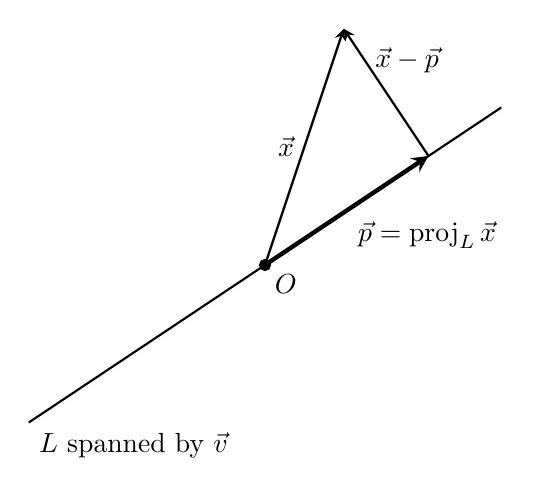
\begin{tikzpicture}
        \draw[thick] (-3, -2) -- (3, 2) node[pos=0, below right]{$L$ spanned by $\vec{v}$};
        \filldraw (0, 0) circle (2pt) node[anchor=north west]{$O$};
        \draw[thick, -stealth] (0, 0) -- (1,3) node[pos=0.5, left]{$\vec{x}$};
        \draw[ultra thick, -stealth] (0, 0) -- (27/13, 18/13) node[pos=0.5, below right]{$\vec{p}=\proj_L \vec{x}$};
        \draw[thick, -stealth] (27/13, 18/13) -- (1, 3) node[pos=0.75, right]{$\vec{x} - \vec{p}$};
    \end{tikzpicture}
    \caption{As seen here, $(\vec{x} - \vec{p}) \cdot \vec{v} = 0$.}
    \label{fig: orthogonal projection onto a line}
\end{wrapfigure}
We will derive the final cumbersome expression in Definition \ref{defn: orthogonal projection}. Since $\vec{x} - \proj_{L}\vec{x}$ is orthogonal to $L$, and since $L$ is parallel to $\vec{v}$, we know that $\vec{x}$ is also orthogonal to $\vec{v}$, i.e. \[\left(\vec{x} - \proj_{L}\vec{x}\right) \cdot \vec{v} = 0.\]
Since $\proj_{L}\vec{x}$ is parallel to $\vec{v}$ by definition, it must be the scalar multiple of $\vec{v}$, i.e. $\proj_{L}\vec{x} = k\vec{v}$ for some $k \in \R$. Then,
\[(\vec{x} - k\vec{v}) \cdot \vec{v} = 0.\]
Distributing the dot product, we have
\[\vec{x}\cdot\vec{v} - k\vec{v} \cdot \vec{v} = 0\]
Adding $k\vec{v}\cdot\vec{v}$ on both sides, we have
\[\vec{x}\cdot\vec{v} = k\vec{v}\cdot\vec{v}.\]
Dividing by $\vec{v} \cdot \vec{v}$ on both sides, we have
\[\frac{\vec{x} \cdot \vec{v}}{\vec{v} \cdot \vec{v}} = k.\]

Now that we have an expression for $k$, we can substitute it in to find that
\[\proj_L\vec{x} = \frac{\vec{x}\cdot\vec{v}}{\vec{v}\cdot\vec{v}} \vec{v},\]
giving rise to the expression in Definition \ref{defn: orthogonal projection}.

\begin{example}
    \nextline
    Let $L$ be the line defined by $y=2x$ in $\R^2$. Let $\vec{a} = \colvec{2}{4}{1}$. Find $\proj_L\vec{a}$.
\begin{solution}
    $L$ is also defined by vector $\vec{v} = \colvec{2}{1}{2}$. Therefore, 
    \[\proj_L\vec{a} = \frac{\colvec{2}{4}{1} \cdot \colvec{2}{1}{2}}{\colvec{2}{1}{2} \cdot \colvec{2}{1}{2}} \colvec{2}{1}{2} = \frac{6}{5}\colvec{2}{1}{2} = \colvec{2}{6/5}{12/5}.\]\hfill \qedsymbol
\end{solution}
\end{example}

Now observe that $\vec{v} \cdot \vec{v} = \left\|\vec{v}\right\|$, which means $\proj_L\vec{x} = \frac{\vec{x} \cdot \vec{v}}{\left\|\vec{v}\right\|} \vec{v}$. For the sake of simplicity, we now make $\vec{u} = \vec{v} / \left\|\vec{v}\right\|$ as a unit vector. Since $\vec{u}$ is parallel to $\vec{v}$, it still spans the same line, i.e. $\proj_L\vec{x} = \frac{\vec{x} \cdot \vec{v}}{\left\|\vec{v}\right\|}\vec{v} = \frac{\vec{x} \cdot \vec{u}}{\left\|\vec{u}\right\|}\vec{u}$. Since $\left\|\vec{u}\right\| = 1$, we have
\[\proj_L\vec{x} = \left(\vec{x} \cdot \vec{u}\right) \vec{u}\]

\begin{theorem}[Orthogonal projection is linear]
    Let $L$ be a line spanned by unit vector $\vec{u}$. Then, $\proj_L:\R^n \to \R^n$ is a linear transformation.
\begin{proof}
    Pick any $\vec{a},\vec{b} \in \R^n$. Then,
    \[
        \proj_L(\vec{a} + \vec{b}) = \left[\left(\vec{a} + \vec{b}\right) \cdot \vec{u}\right]\vec{u} 
        = \left[\vec{a}\cdot\vec{u} + \vec{b}\cdot\vec{u}\right]\vec{u} 
        = \left(\vec{a}\cdot\vec{u}\right)\vec{u} + \left(\vec{b}\cdot\vec{u}\right)\vec{u} 
        = \proj_L\vec{a} + \proj_L\vec{b}.
    \]
    Let $c\in\R$ be a scalar. Then,
    \begin{align*}
        \proj_L(c\vec{a}) = \left(c\vec{a} \cdot \vec{u}\right)\vec{u} = c(\vec{a}\cdot\vec{u})\vec{u} = c\proj_L\vec{a}.
    \end{align*}
    Hence $\proj_L$ is a linear transformation.
\end{proof}
\end{theorem}

Now we limit ourselves to the discussion of $\R^2$ for the sake of simplicity, i.e. let $\proj_L:\R^2 \to \R^2$. Also, let $\vec{u} = \vecxx[u]$ (reminder: $u$ is a unit vector describing $L$). Then, we have
\begin{align*}
    \proj_L\sbvec{1} &= \left(\colvec{2}{1}{0} \cdot \vecxx[u]\right)\vecxx[u] = \colvec{2}{u_1^2}{u_1u_2}, \text{ and} \\
    \proj_L\sbvec{2} &= \left(\colvec{2}{0}{1} \cdot \vecxx[u]\right)\vecxx[u] = \colvec{2}{u_1u_2}{u_2^2},
\end{align*}
leading to Theorem \ref{thm: 2d projection matrix}.
\begin{theorem}[Matrix for 2d orthogonal projection]
    \label{thm: 2d projection matrix}
    Let $L$ be a line in $\R^2$ spanned by unit vector $\vec{u} = \vecxx[u]$. Then, \[\proj_L\vec{x} = \begin{bmatrix}u_1^2 & u_1u_2 \\ u_1u_2 & u_2^2\end{bmatrix}\vec{x}\]
    for all $\vec{x} \in \R^2$.
\end{theorem}
Theorem \ref{thm: projection matrix generalized} generalizes Theorem \ref{thm: 2d projection matrix} to $\R^n$.
\begin{theorem}[Generalization of projection matrix]
    \label{thm: projection matrix generalized}
    \nextline
    Let $L$ be a line in $\R^n$ spanned by unit vector $\vec{u} = \vecxxdx[u]$. Let $\mat{M}=\cmat[a]$ such that $\proj_L\vec{x} = \mat{M}\vec{x}$ for all $\vec{x} \in \R^n$. Then,
    $\vec{a}_i = u_i \vec{u}$
    for all $1 \leq i \leq n$.
\begin{proof}
    Let $1 \leq i \leq n$. Then,
    \[\vec{a}_i = \proj_L\sbvec{i} = \left(\sbvec{i}\vecxxdx[u]\right)\cdot \vecxxdx[u] = u_i \vecxxdx[u] = u_i \vec{u}.\]
\end{proof}
\end{theorem}
\begin{example}
    \label{expl: projection to x-axis}
    Find the matrix of the orthogonal projection to the $x$-axis in $\R^2$ using Theorem \ref{thm: 2d projection matrix}.
\begin{solution}
    The vector $\vec{u} = \colvec{2}{1}{0}$ is a unit vector spanning the $x$-axis, for $u_1=1$ and $u_2=0$. By Theorem \ref{thm: 2d projection matrix},
    \begin{align*}
        \proj_L \vec{x} &= \begin{bmatrix}
            u_1^2 & u_1u_2 \\ u_1u_2 & u_2^2
        \end{bmatrix} \vec{x} \\
        &= \begin{bmatrix}
            1&0 \\ 0&0
        \end{bmatrix} \vec{x}.
    \end{align*}
    Hence the matrix of transformation is $\begin{bmatrix} 1&0 \\ 0&0 \end{bmatrix}$. Now if we let $\vec{x} = \vecxx$ and multiply the matrix-vector product out, we have
    \[\proj_L \vec{x}  = \begin{bmatrix}1&0 \\ 0&0\end{bmatrix} \vecxx = \colvec{2}{x_1}{0},\] i.e. the $y$-component of $\vec{x}$ disappears, only leaving the $x$-component. \hfill \qedsymbol 
\end{solution}
\end{example}

Sometimes, it would also be useful to orthogonally project a vector to a plane $V$ with equation $ax+by+cz=0$. From this equation, we can see that the normal vector is (assume unit vector) $\vec{n} = \colvec{3}{u_1}{u_2}{u_3}$. Let $L^{\perp}$ be the line spanned by $\vec{n}$. Pick any $\vec{v} \in \R^3$. We see from Figure \ref{fig: orthogonal projection to plane} that
\[\proj_V\vec{v} + \proj_{L^{\perp}} \vec{v} = \vec{v},\]
i.e. $\proj_V\vec{V} = \vec{v} - \proj_{L^{\perp}}\vec{v}$. 

By Theorem \ref{thm: projection matrix generalized}, 
\[\proj_{L^{\perp}}\vec{v} = \begin{bmatrix}u_1^2 & u_1u_2 & u_1u_3 \\ u_1u_2 & u_2^2 & u_2u_3 \\ u_1u_3 & u_2u_3 & u_3^2\end{bmatrix} \vec{v};\]
by Theorem \ref{thm: identity matrix gives identity},
\[\vec{v} = \idmat[3]\vec{v}.\]
Therefore,
\begin{align*}
    \proj_V\vec{v} &= \vec{v} - \proj_{L^{\perp}}\vec{v} \\
    &= \idmat[3]\vec{v} - \begin{bmatrix}u_1^2 & u_1u_2 & u_1u_3 \\ u_1u_2 & u_2^2 & u_2u_3 \\ u_1u_3 & u_2u_3 & u_3^2\end{bmatrix}\vec{v} \\
    &= \begin{bmatrix}1-u_1^2 & -u_1u_2 & -u_1u_3 \\ -u_1u_2 & 1-u_2^2 & -u_2u_3 \\ -u_1u_3 & -u_2u_3 & 1-u_3^2\end{bmatrix} \vec{v}.
\end{align*}

\begin{figure}
    \centering
    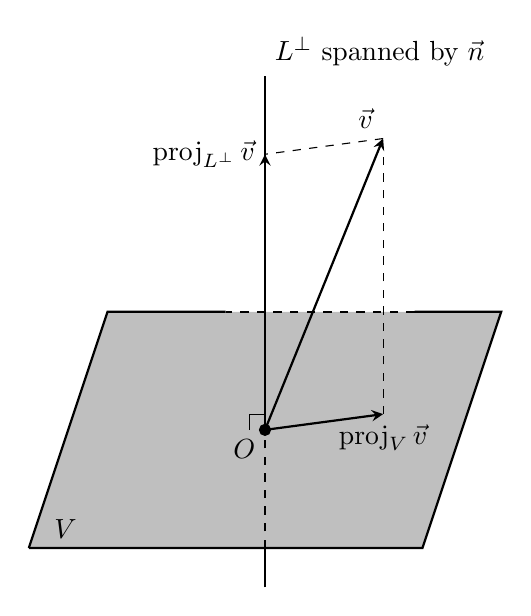
\begin{tikzpicture}
        \draw[fill=lightgray, draw=none] (0,0) -- (5,0) -- (6,3) -- (1, 3) -- cycle;
        \draw[thick] (0,0) -- (5,0) -- (6,3) -- (4.9, 3); % -- (1,4) -- cycle;
        \draw[thick,dashed] (4.9, 3) -- (2.5,3);
        \draw[thick] (2.5, 3) -- (1,3) -- (0,0);
        \node[anchor = south west] at (0.2, 0) {$V$}; 
        \filldraw (3,1.5) circle (2pt) node[anchor=north east]{$O$};
        \draw (3,1.5) -- (3,6) node[anchor=south west]{$L^{\perp}$ spanned by $\vec{n}$};
        \draw[dashed] (3,0) -- (3,1.5);
        \draw (3,-0.5) -- (3,0);
        \draw (3, 1.7) -- (2.8, 1.7) -- (2.8, 1.5);
        \draw[thick, -stealth] (3, 1.5) -- (4.5, 5.2) node[anchor=south east]{$\vec{v}$};
        \draw[dashed] (4.5, 5.2) -- (3, 5);
        \draw[thick, -stealth] (3,1.5) -- (3,5) node[anchor = east]{$\proj_{L^{\perp}}\vec{v}$};
        \draw[dashed] (4.5, 1.7) -- (4.5, 5);
        \draw[thick, -stealth] (3,1.5) -- (4.5, 1.7) node[anchor = north]{$\proj_{V} \vec{v}$};
    \end{tikzpicture}
    \caption{As seen here, $\vec{v} = \proj_V\vec{v} + \proj_{L^{\perp}}\vec{v}$.}
    \label{fig: orthogonal projection to plane}
\end{figure}

\subsection{Reflection}
Consider line $L$ in $\R^n$ running through the origin defined by the span of unit vector $\vec{u} \in \R^n$. Let $\vec{x} \in \R^n$ be an arbitrary vector. Then, $\vec{x} = \vec{x}^{\parallel} + \vec{x}^{\perp}$ for some $\vec{x}^{\parallel}$ parallel to $L$ and $\vec{x}^{\perp}$ orthogonal to $L$.
\begin{definition}[reflection]
    We define $\vecref_L \vec{x}$ as the reflection of $\vec{x}$ via line $L$. We have \[\vecref_L \vec{x} = \vec{x}^{\parallel} - \vec{x}^{\perp}.\]
\end{definition}
Since $\vecref_L \vec{x} = \vec{x}^{\parallel} - \vec{x}^{\perp}$, and $\vec{x} = \vec{x}^{\parallel} + \vec{x}^{\perp}$, we add the two expressions to yield \[\vecref_L \vec{x} + \vec{x} = 2\vec{x}^{\parallel}\] i.e. \[\vecref_L \vec{x} = 2\vec{x}^{\parallel} - \vec{x}.\]

By Definition \ref{defn: orthogonal projection}, we have $\vec{x}^{\parallel} = \proj_L \vec{x}$, since $\vec{x}^{\parallel}$ is parallel to $L$ and $\vec{x} - \vec{x}^{\parallel} = \vec{x}^{\perp}$ is orthogonal to $L$. Hence
\[\vecref_L \vec{x} = 2\proj_L \vec{x} - \vec{x}.\]

For the sake of simplicity, we restrict ourselves to $\R^2$. Then, by Theorems \ref{thm: 2d projection matrix} and \ref{thm: identity matrix gives identity}, we have
\begin{align*}
    \vecref_L \vec{x} = 2\begin{bmatrix}u_1^2 & u_1u_2 \\ u_1u_2 & u_2^2 \end{bmatrix}\vec{x} - \begin{bmatrix}1 & 0 \\ 0 & 1 \end{bmatrix}\vec{x}
\end{align*}
leading to Theorem \ref{thm: mat for 2d ref}.
\begin{theorem}[Matrix for 2d reflection]
    \label{thm: mat for 2d ref}
    Let $L$ be a line in $\R^2$ spanned by unit vector $\vec{u} = \vecxx[u]$. Then, \[\vecref_L \vec{x} = \begin{bmatrix}2u_1^2 - 1 & 2u_1u_2 \\ 2u_1u_2 & 2u_2^2 - 1 \end{bmatrix} \vec{x}.\]
\end{theorem}
\begin{example}
    Find the matrix of the reflection about the $x$-axis in $\R^2$ using Theorem \ref{thm: mat for 2d ref}.
\begin{solution}
    Unit vector $\vec{u} = \colvec{2}{1}{0}$ spans the $x$-axis, so we have
    \[\vecref_L \vec{x} = \begin{bmatrix}2u_1^2 - 1 & 2u_1u_2 \\ 2u_1u_2 & 2u_2^2 - 1 \end{bmatrix} \vec{x} = \begin{bmatrix}1 & 0 \\ 0 & -1\end{bmatrix}.\]
    Hence $\begin{bmatrix}1 & 0 \\ 0 & -1\end{bmatrix}$ is a matrix for the reflection about the $x$-axis. Let $\vec{x} = \vecxx$; if we multiply out the matrix-vector product, we have
    \[\begin{bmatrix}1 & 0 \\ 0 & -1\end{bmatrix} \vecxx = \colvec{2}{x_1}{-x_2},\] i.e. the $y$-component flips and the $x$-component stays the same. \hfill \qedsymbol
\end{solution}
\end{example}

Now, let $a=2u_1^2 - 1$ and $b=2u_1u_2$. Since $\vec{u}$ is a unit vector, we know $u_1^2 + u_2^2 = 1$, i.e. $u_2^2 = 1 - u_1^2$. Then,
\[
    2u_2^2 - 1= 2\left(1 - u_1^2\right) - 1 = 2 - 2u_1^2 - 1 = 1 - 2u_1^2 = -a.
\]
Also note that $a^2 + b^2 = 1$, leading to Theorem \ref{thm: ref abb-a}.
\begin{theorem}[Another representation of reflections]
    \label{thm: ref abb-a}
    Let $L$ be a line passing through the origin in $\R^2$. Then, the matrix of $\vecref_L$ has form $\begin{bmatrix}a & b \\ b & -a\end{bmatrix}$ for $a^2 + b^2 = 1$. Conversely, any matrices of form $\begin{bmatrix}a & b \\ b & -a\end{bmatrix}$ represents a reflection transformation via some line $L$ in $\R^2$.
\end{theorem}

\subsection{Identifying Types of Linear Transformations}
Given a transformation matrix, we would want to know which type of transformation it is. It's usually useful to think about the transformations' effects on the differences of two vectors. Here are several examples aimed at identifying linear transformations and interpreting them geometrically.
\begin{example}
    \label{expl: indentify reflection transformation}
    Let \[\mat{A} = \frac{1}{5} \begin{bmatrix}-3 & 4 \\ 4 & 3\end{bmatrix}.\]
    Let $T(\vec{x}) = \mat{A}\vec{x}$. Is $T$ a rotation, reflection, projection, or scaling? Interpret $T$ geometrically.
\begin{solution}
    If $T$ were to be a projection transformation, then $\left\{T(\vec{x}) \suchthat \vec{x} \in \R^2\right\}$ would be a line, i.e. all $\vec{v} \in \left\{T(\vec{x}) \suchthat \vec{x} \in \R^2\right\}$ must be parallel. However, from the transformation matrix, we see that $T(\sbvec{1}) = \frac{1}{5}\colvec{2}{-3}{4}$ and $T(\sbvec{2}) = \frac{1}{5}\colvec{2}{4}{3}$. They are not parallel, i.e. $T$ does not represent a projection transformation. 
    
    If $T$ were to be a rotation transformation, then the matrix entry on the top-right and the matrix entry on the top-left should have different sign (see Theorem \ref{thm: rotation a-bba}), which is not what we observe here. Hence $T$ is not a rotation transformation. 
    
    Let $a = -3/5$ and $b = 4/5$. Then, $\mat{A} = \begin{bmatrix}a & b \\ b & -a\end{bmatrix}$ for $a^2 + b^2 = 1$. By Theorem \ref{thm: ref abb-a}, $T$ represents a reflection transformation. 
    
    To figure out the line $L$ about which $T$ reflects, observe that if $\vec{x}$ is parallel to $L$, then $T(\vec{x}) = \vec{x}$. We can use this fact to solve for a vector $\vec{x}$ parallel to $L$, and hence defining the line.
    
    We set up equation
    \[\frac{1}{5} \begin{bmatrix}-3 & 4 \\ 4 & 3\end{bmatrix}\vecxx = \vecxx,\]
    i.e.
    \begin{align*}
        \frac{1}{5}\colvec{2}{-3x_1+4x_2}{4x_1+3x_2} = \vecxx,
    \end{align*}
    i.e.
    \begin{align*}
        -8x_1 + 4x_2 &= 0 \\
        4x_1 - 2x_2 &= 0.
    \end{align*}
    Solving this system of equations using row-reduced echelon form, we yield $x_2 = 2x_1$ as a solution. Hence, the line about which the reflection occurs is $y=2x$. \hfill \qedsymbol
\end{solution}
\end{example}

\begin{example}
    \label{expl: identifying rotation transformation}
    Consider matrix $\mat{A} = \begin{bmatrix}-1/2 & -\sqrt{3}/2 \\ \sqrt{3}/2 & -1/2 \end{bmatrix}$, and linear transformation $T(\vec{x}) = \mat{A}\vec{x}$. Interpret $T$ geometrically.
\begin{solution}
    $T$ is definitely not a projection transformation, because the column vectors are not parallel (see Example \ref{expl: indentify reflection transformation}).
    
    By Theorem \ref{thm: rotation a-bba}, since the numbers on the main diagonal are of the same sign, while those on the antidiagonal have different signs, and $\left(\frac{-1}{2}\right)^2 + \left(\frac{-\sqrt{3}}{2}\right)^2 = 1$, $T$ represents a rotation transformation. Then, $\cos\theta = \frac{-1}{2}$ while $\sin\theta = \frac{\sqrt{3}}{2}$, yielding $\theta = \frac{2\pi}{3}$. Therefore, $T$ is a linear transformation rotating $\vec{x}$ counterclockwise by $2\pi/3$ radians, or $120^{\circ}$. \hfill \qedsymbol
\end{solution}
\end{example}



\section{Composing Linear Transformations}
Let $S:X \to Y$, $T: Y \to Z$ be transformations, for $X \subseteq \R^n$, $Y\subseteq \R^m$, and $Z \subseteq \R^l$.
\begin{definition}[composition of transformations]
    We define $T \circ S: X \to Z$ as a transformation such that for all $\vec{x} \in X$, $(T \circ S)(\vec{x}) = T\left(S\left(\vec{x}\right)\right)$. We say $T \circ S$ is the \textbf{composition} of $T$ with $S$.
\end{definition}
Now suppose $S$ and $T$ are linear transformations. Theorem \ref{thm: composition of linear transformations is linear} tells us that $T \circ S$ is a linear transformation.
\begin{theorem}[Composition of linear transformations is linear]
    \label{thm: composition of linear transformations is linear}
    Let $S:X \to Y$ and $T: Y \to Z$ be linear transformations for $X \subseteq \R^n$, $Y \subseteq \R^m$, and $Z \subseteq \R^l$. Then, $T \circ S$ is a linear transformation.
\begin{proof}
    Pick any $\vec{a},\vec{b} \in X$. Then,
    \begin{align*}
        \left(T \circ S\right)\left(\vec{a} + \vec{b}\right) &= T\left(S\left(\vec{a} + \vec{b}\right)\right) & \text{defn. of composition} \\
        &= T\left(S\left(\vec{a}\right) + S\left(\vec{b}\right)\right) & \text{$S$ is linear} \\
        &= T\left(S\left(\vec{a}\right)\right) + T\left(S\left(\vec{b}\right)\right) & \text{$T$ is linear} \\
        &= \left(T\circ S\right)\left(\vec{a}\right) + \left(T\circ S\right)\left(\vec{b}\right). & \text{defn. of composition}
    \end{align*}
    Now pick $c \in \R$ to be a scalar. Then,
    \begin{align*}
        \left(T \circ S\right)\left(c\vec{a}\right) &= T\left(S\left(c\vec{a}\right)\right) & \text{defn. of composition} \\
        &= T\left(cS\left(\vec{a}\right)\right) & \text{$S$ is linear} \\
        &= cT\left(S\left(\vec{a}\right)\right) & \text{$T$ is linear} \\
        &= c\left(T \circ S\right)\left(\vec{a}\right). & \text{defn. of composition}
    \end{align*}
    By definition, then, $T \circ S$ is a linear transformation.
\end{proof}
\end{theorem}

Since $T$ is linear, there exists an $m \times n$ matrix $\mat{A}$ and $l \times m$ matrix $\mat{B}$ such that $T(\vec{x}) = \mat{A} \vec{x}$ and $S(\vec{x}) = \mat{B}\vec{x}$. Since $T \circ S$ is a linear transformation, by Theorem \ref{thm:lt=mvp}, there exists an $l \times n$ matrix $\mat{C}$ such that $(T \circ S) = \mat{C}\vec{x}$. We have
\[\left(T\circ S\right)(\vec{x}) = T\left(S\left(\vec{x}\right)\right) = T\left(\mat{A}\vec{x}\right) = \mat{B}\left(\mat{A}\vec{x}\right) = \mat{C}\vec{x}.\]
We will now find $\mat{C}$.
\[
    \mat{C} = \begin{bmatrix}\vert & \vert && \vert \\ \mat{B}\left(\mat{A}\sbvec{1}\right) & \mat{B}\left(\mat{A}\sbvec{2}\right) & \cdots & \mat{B}\left(\mat{A}\sbvec{n}\right) \\ \vert & \vert && \vert\end{bmatrix}.
\]

Let $\mat{A} = \cmat[a]$. Since $\mat{A}\sbvec{i} = \vec{a}_i$, 
\[
    \mat{C} = \begin{bmatrix}\vert & \vert && \vert \\ \mat{B}\vec{a}_1 & \mat{B}\vec{a}_2 & \cdots & \mat{B}\vec{a}_n \\ \vert & \vert && \vert\end{bmatrix},
\]
leading to Theorem \ref{thm:composition of linear transformations mvp}.
\begin{theorem}[Matrix of composition of linear transformations]
    \label{thm:composition of linear transformations mvp}
    Let $T:X \to Y$, $S:Y \to Z$ be linear transformations for $X \subseteq \R^n, Y\subseteq \R^m, Z \subseteq \R^l$. Let $\mat{A} = \cmat[a]$ be an $m \times n$ matrix such that $S(\vec{x}) = \mat{A}\vec{x}$. Let $\mat{B}$ be a $l \times m$ matrix such that $T(\vec{x}) = \mat{B} \vec{x}$. Then,
    \[(T \circ S) = \mat{C}\vec{x}\] for \[\mat{C} = \begin{bmatrix}\vert & \vert && \vert \\ \mat{B}\vec{a}_1 & \mat{B}\vec{a}_2 & \cdots & \mat{B}\vec{a}_n \\ \vert & \vert && \vert\end{bmatrix}.\]
\end{theorem}
Theorem \ref{thm:composition of linear transformations mvp}, now, allows us to define the product of two matrices, in Definition \ref{defn: product of two matrices}.
\begin{definition}[product of two matrices]
    \label{defn: product of two matrices}
    Let $\mat{A} = \cmat[a]$ be an $m \times n$ matrix. Let $\mat{B}$ be an $l \times m$ matrix. Then, we define the \textbf{product of $\pmb{\mat{B}}$ and $\pmb{\mat{A}}$} as $\mat{B}\mat{A} = \begin{bmatrix}\vert & \vert && \vert \\ \mat{B}\vec{a}_1 & \mat{B}\vec{a}_2 & \cdots & \mat{B}\vec{a}_n \\ \vert & \vert && \vert\end{bmatrix}$. $\mat{B}\mat{A}$ is an $l \times n$ matrix. The $ij$-th entry of $\mat{B}\mat{A}$ equals to the dot product between the $i$-th row of $\mat{B}$ and the $j$-th column of $\mat{A}$.
\end{definition}
\begin{remark}
    Let $\mat{A},\mat{B}$ be matrices. $\mat{AB}$ is defined if and only if $\mat{A}$ has the same number of columns as $\mat{B}$ has rows.
\end{remark}

% TODO: Explain the last statement of defn of product of two matrices.

We can now define powers of matrices using matrix multiplication, similar to how we defined $n^k = \underbrace{n \times n \times \cdots \times n}_{\text{$k$ times}}$.

\begin{definition}[power of matrices]
    Let $\mat{A}$ be an $n \times n$ matrix. Then, we define $\mat{A}^0 = \idmat[n]$, $\mat{A}^1 = \mat{A}$, and $\mat{A}^n = \mat{A} \mat{A}^{n-1}$ for $n \geq 3$. Succinctly, 
    \[\mat{A}^n = \underbrace{\mat{A}\cdots\mat{A}}_{n \text{ times}}.\]
\end{definition}
\begin{example}
    \label{expl:find matrix product}
    Let $\mat{A} = \begin{bmatrix} 1 & -1 & 2 \\ 0 & -2 & 1 \end{bmatrix}$ and $\mat{B} = \begin{bmatrix}1&0&1&1 \\ 2&0&1&-1 \\ 3&1&0&2\end{bmatrix}$. Find $AB$. If it's undefined, indicate so.
\begin{solution}
    Let $\mat{A}\mat{B} = \begin{bmatrix}\vert & \vert & \vert & \vert \\ \vec{c}_1 & \vec{c}_2 & \vec{c}_3 & \vec{c}_4 \\ \vert & \vert & \vert & \vert\end{bmatrix}$. Then,
    \begin{itemize}
        \item $\vec{c}_1 = \begin{bmatrix} 1 & -1 & 2 \\ 0 & -2 & 1 \end{bmatrix}\colvec{3}{1}{2}{3} = \colvec{2}{5}{-1}$,
        \item $\vec{c}_2 = \begin{bmatrix} 1 & -1 & 2 \\ 0 & -2 & 1 \end{bmatrix}\colvec{3}{0}{0}{1} = \colvec{2}{2}{1}$,
        \item $\vec{c}_3 = \begin{bmatrix} 1 & -1 & 2 \\ 0 & -2 & 1 \end{bmatrix}\colvec{3}{1}{1}{0} = \colvec{2}{0}{-2}$, and
        \item $\vec{c}_4 = \begin{bmatrix} 1 & -1 & 2 \\ 0 & -2 & 1 \end{bmatrix}\colvec{3}{1}{-1}{2} = \colvec{2}{6}{4}$.
    \end{itemize}
    Hence $\mat{A}\mat{B} = \begin{bmatrix}5&2&0&6\\-1&1&-2&4\end{bmatrix}$.
    \hfill \qedsymbol
\end{solution}
\end{example}

\begin{example}
    Using the same matrices in Example \ref{expl:find matrix product}, find $\mat{B}\mat{A}$. Again, if it's not defined, indicate so.
\begin{solution}
    Observe that $\mat{B}$ has four columns, while $\mat{A}$ has two rows. Hence $\mat{B}\mat{A}$ is undefined. \hfill \qedsymbol
\end{solution}

\end{example}

\begin{remark}
    Let $\mat{A},\mat{B}$ be matrices, and suppose $\mat{AB}$ and $\mat{BA}$ are both defined. It is not necessarily the case that $\mat{AB} = \mat{BA}$, i.e. we don't have the commutative property. However, there exist cases where $\mat{AB} = \mat{BA}$. See Definition \ref{defn: commute matrix}.
\end{remark}
\begin{definition}[commute]
    \label{defn: commute matrix}
    We say that matrices $\mat{A},\mat{B}$ \textbf{commute} if and only if $\mat{AB},\mat{BA}$ are defined and $\mat{AB}=\mat{BA}$.
\end{definition}

We will now list a few important properties of matrix multiplication. 
\begin{theorem}[Associative and distributive property of matrix products]
    \label{thm: matrix product associative and distributive properties}
    Let $\mat{A},\mat{B},\mat{C}$ be matrices. Then, 
    \begin{itemize}
        \item $\mat{A}\mat{B}\mat{C} = \left(\mat{A}\mat{B}\right)\mat{C} = \mat{A}\left(\mat{B}\mat{C}\right)$, and
        \item $\mat{A}(\mat{B} + \mat{C}) = \mat{AB} + \mat{AC}$
    \end{itemize}
    if the products are defined. In addition, if $\mat{B}\mat{A}$ and $\mat{C}\mat{A}$ are both defined, then $(\mat{B}\mat{C})\mat{A} = \mat{BA} + \mat{CA}$.
\end{theorem}
\begin{corollary}[Associative property of linear transformations]
    Let $H:W \to X$, $G:X \to Y$, $F: Y \to Z$ be linear transformations for $W \subseteq \R^m,X \subseteq \R^m, Y \subseteq \R^p, Z \subseteq \R^q$, and suppose $(H \circ G)$ and $(G \circ F)$ are both defined and valid compositions. Then, $(H \circ G) \circ F = H \circ (G \circ F) = H \circ G \circ F$, i.e. they are the same transformations.
\begin{proof}
    The proof follows directly from Theorem \ref{thm: matrix product associative and distributive properties} and \ref{thm:lt=mvp}. Write $H$, $G$, and $F$ as their matrix-vector product forms, and use the associativity of matrix products to show the claim.
\end{proof}
\end{corollary}

As the name suggests, the identity matrix should give identity. In Theorem \ref{thm: identity matrix gives identity}, we have shown that $\idmat[n]\vec{v} = \vec{v}$ for all $\vec{v} \in \R^n$. Theorem \ref{thm: matrix product with identity matrix} tells us that the same rules apply on matrix multiplication.
\begin{theorem}[Matrix product with identity matrix]
    \label{thm: matrix product with identity matrix}
    Let $\mat{A}$ be an $n \times n$ matrix. Then, 
    \[\idmat[n]\mat{A} = \mat{A}\idmat[n] = \mat{A}.\]
\end{theorem}


\subsection{Transposes, Rowspaces, Left Nullspaces, and Matrix Products}
\label{section: transposes, rowspaces, left nullspaces, and matrix products}
We will now study matrix and vector transposes' effects on matrix products and matrix-vector products.
\begin{theorem}[Transpose of matrix products]
    \label{thm: transpose of matrix products}
    Let $\mat{A}$ be an $m \times n$ matrix, and $\mat{B}$ be an $n \times m$ matrix. Then,
    \[\left(\mat{A}\mat{B}\right)^T = \mat{B}^T\mat{A}^T.\]
\begin{proof}
    The proof comes directly from comparing the $ij$-th entry of $\mat{A}\mat{B}$ and the $ji$-th entry of $\mat{B}^T\mat{A}^T$, and concluding that they are equal. Hence the $ji$-th entry of $\left(\mat{A}\mat{B}\right)^T$ equals to the $ji$-th entry of $\mat{B}^T\mat{A}^T$, and hence $\left(\mat{A}\mat{B}\right)^T = \mat{B}^T\mat{A}^T$.
\end{proof}
\end{theorem}

Now, let $\vec{v} = \vecxxdx[v]$ be a column vector. Then, $\vec{v}$ is essentially an $n \times 1$ matrix. Let's take its transpose:
\[\vec{v}^T = \begin{bmatrix}v_1 & v_2 & \cdots & v_n\end{bmatrix}\]
which is essentially an $1 \times n$ matrix.

Let $\vec{w} = \vecxxdx[w]$. We have
\[\vec{v}^T\vec{w} = \underbrace{\begin{bmatrix}v_1 & v_2 & \cdots & v_n\end{bmatrix}}_{1 \times n} \underbrace{\vecxxdx[w]}_{n \times 1}=v_1w_1 + v_2w_2 + \cdots + v_nw_n = \vec{v}\cdot\vec{w}.\]

We summarize this result in Theorem \ref{thm: vector transpose and dot product}.

\begin{theorem}[Vector transpose and dot product]
    \label{thm: vector transpose and dot product}
    Let $\vec{v},\vec{w} \in \R^n$. Then,
    \[\vec{v} \cdot \vec{w} = \vec{v}^T\vec{w}.\]
\end{theorem}

We can now build on this idea. Let $\mat{A}$ be an $m \times n$ matrix, and let $\vec{x} \in \R^n$. Then, $\mat{A}\vec{x} \in \R^m$. Therefore, if $\vec{y} \in \R^m$, $(\mat{A}\vec{x})\cdot\vec{y}$ is defined. We can compute
\begin{align*}
    (\mat{A}\vec{x})\cdot\vec{y} &= (\mat{A}\vec{x})^T\vec{y} & \text{Theorem \ref{thm: vector transpose and dot product}} \\
    &= \left(\vec{x}^T\mat{A}^T\right)\vec{y} & \text{Theorem \ref{thm: transpose of matrix products}} \\
    &= \vec{x}^T\left(\mat{A}^T\vec{y}\right) & \text{Matrix Products are Associative} \\
    &= \vec{x}\left(\mat{A}^T\vec{y}\right). & \text{Theorem \ref{thm: vector transpose and dot product}}
\end{align*}

We now summarize this result in Theorem \ref{thm: matrix vector product and transpose}.

\begin{theorem}[Matrix vector product and transpose]
    \label{thm: matrix vector product and transpose}
    Let $\mat{A}$ be an $m \times n$ matrix, and let $\vec{x} \in \R^n$ and $\vec{y} \in \R^m$. Then,
    \[\left(\mat{A}\vec{x}\right)\cdot\vec{y} = \vec{x}\left(\mat{A}^T\vec{y}\right).\]
\end{theorem}

Recall that we defined the left nullspace, or left kernel, of a matrix in Definition \ref{defn: left null space; left kernel}. We will now derive an equation that can be used to find the left kernel of a matrix. 

Let $\mat{A}$ be an $m \times n$ matrix. Then, by definition, the left kernel of $\mat{A}$ is
\[\kernel\mat{A}^T = \left\{\vec{x} \in \R^m \suchthat \mat{A}^T\vec{x} = \vec{0}\right\}.\]
Let's take the expression $\mat{A}^T\vec{x}=\vec{0}$, and transpose both sides, yielding
\[\left(\mat{A}^T\vec{x}\right)^T = \vec{0}^T \Longleftrightarrow \vec{x}^T \left(\mat{A}^T\right)^T = \vec{0}^T.\]
Since $\left(\mat{A}^T\right)^T = \mat{A}$, we have
\[\vec{x}^T\mat{A} = \vec{0}^T.\]

This motivates Theorem \ref{thm: expression for left nullspace and left kernel}.

\begin{theorem}[Expression for left nullspace and left kernel]
    \label{thm: expression for left nullspace and left kernel}
    Let $\mat{A}$ be an $m \times n$ matrix. Then, the left kernel, or the left nullspace, of $\mat{A}$ is
    \[\kernel\mat{A}^T = \left\{\vec{x} \in \R^m \suchthat \vec{x}^T\mat{A} = \vec{0}^T\right\}.\]
\end{theorem}

\subsection{Analyzing Linear Transformation Composition}
We start with an example of analyzing patterns of powers of a rotation transformation in Example \ref{expl: compute and interpret rotation composition}.
\begin{example}
\label{expl: compute and interpret rotation composition}
    Consider matrix $\mat{A} = \begin{bmatrix}-1/2 & -\sqrt{3}/2 \\ \sqrt{3}/2 & -1/2 \end{bmatrix}$, and linear transformation $T(\vec{x}) = \mat{A}\vec{x}$. In Example \ref{expl: identifying rotation transformation}, we have concluded that $T$ represents a rotation transformation of rotating $\vec{x}$ counterclockwise by $2\pi / 3$ radians. Now, compute and geometrically interpret linear transformations defined by matrices $\mat{A}^2$, $\mat{A}^3$, $\mat{A}^4$, and $\mat{A}^{2020}$.
\begin{solution}
    $\mat{A}^2$ represents applying $T$ on $\vec{x}$ twice, i.e. rotating $\vec{x}$ counterclockwise for a total of $4\pi / 3$ radians. By the unit circle, $\cos\frac{4\pi}{3} = -\frac{1}{2}$, and $\sin\frac{4\pi}{3} = -\frac{\sqrt{3}}{2}$. Hence, by Theorem \ref{thm: rotation a-bba}, $\mat{A}^2 = \begin{bmatrix}-1/2 & \sqrt{3}/2 \\ -\sqrt{3}/2 & -\frac{1}{2}\end{bmatrix}.$
    
    $\mat{A}^3$ represents applying $T$ on $\vec{x}$ three times, i.e. rotating counterclockwise $2\pi / 3$ radians three times, which is equivalent to not rotating at all, i.e. $\mat{A}^3 = \idmat[2]$. 
    
    $\mat{A}^4 = \mat{A}^3\mat{A} = \idmat[2]\mat{A} = \mat{A}$, i.e. $\mat{A}^4$ represents the same transformation as $\mat{A}$, rotating $\vec{x}$ counterclockwise by $2\pi / 3$ radians.
    
    $\mat{A}^{2020}$ represents rotating $\vec{x}$ by $2\pi / 3$ radians for a total of 2020 times. Since every three times of rotation represents not rotating at all, and since $2020 \bmod 3 = 1$, $\mat{A}^{2020} = \mat{A}^1 = \mat{A}$, i.e. $\mat{A}^{2020}$ represents rotating $\vec{x}$ counterclockwise by $2\pi / 3$ radians. \hfill \qedsymbol
\end{solution}
\end{example}

Now we will study an example where composing linear transformations by itself does not change the result in Example \ref{expl: idempotent linear transformations}, which we call \textit{idempotent linear transformations}.
\begin{example}
    \label{expl: idempotent linear transformations}
    Let line $L$ be spanned by unit vector $\vec{u} = \vecxx[u]$. Compute the matrix for linear transformation $\proj_L \circ \proj_L$.
\begin{solution}
    By Theorem \ref{thm: 2d projection matrix},  $$\mat{M} = \begin{bmatrix} u_1^2 & u_1u_2 \\ u_1u_2 & u_2^2 \end{bmatrix}$$ is the matrix for $\proj_L$. Therefore, $\mat{M}\mat{M}$ is the matrix for $\proj_L \circ \proj_L$. 
    
    Computing $\mat{M}\mat{M}$,
    \begin{align*}
        \mat{M}\mat{M} &= \begin{bmatrix} u_1^2 & u_1u_2 \\ u_1u_2 & u_2^2 \end{bmatrix} \begin{bmatrix} u_1^2 & u_1u_2 \\ u_1u_2 & u_2^2 \end{bmatrix} \\
        &= \begin{bmatrix}u_1^4 + u_1^2u_2^2 & u_1^3u_2 + u_1u_2^3 \\
        u_1^3u_2 + u_1u_2^3 & u_1^2u_2^2 + u_2^4\end{bmatrix} \\
        &= \begin{bmatrix}u_1^2(u_1^2 + u_2^2) & u_1u_2(u_1^2 + u_2^2) \\
        u_1u_2(u_1^2 + u_2^2) & u_2^2(u_1^2+u_2^2)\end{bmatrix}.
    \end{align*}
    Since $\vec{u}$ is a unit vector, $u_1^2 + u_2^2 = 1$, i.e. 
    \[\mat{M}\mat{M} = \mat{M}^2 = \mat{M}.\]
    
    This result is very powerful: since $\mat{M}^2 = \mat{M}$, $\mat{M}^3 = \mat{M}^2\mat{M} = \mat{M}\mat{M} = \mat{M}^2 = \mat{M}$, etc. Orthogonal projections are idempotent in the sense that applying it once is no different from applying it multiple times. Another example of an idempotent function is the absolute value function. \hfill \qedsymbol
\end{solution}
\end{example}

Now we will study a case where applying two linear transformations one after another is equivalent to applying another transformation once, in Example \ref{expl: two reflections equal to one rotation}.
\begin{example}
    \label{expl: two reflections equal to one rotation}
    Let $\mat{M}_1 = \begin{bmatrix}a_1 & b_1 \\ b_1 & -a_1\end{bmatrix}$ and $\mat{M}_2 = \begin{bmatrix}a_2 & b_2 \\ b_2 & -a_2\end{bmatrix}$ for $a_1^2 + b_1^2 = a_2^2 + b_2^2 = 1$. Let $T_1(\vec{x}) = \mat{M}_1 \vec{x}$ and $T_2(\vec{x}) = \mat{M}_2\vec{x}$. By Theorem \ref{thm: ref abb-a}, $T_1$ and $T_2$ are reflection transformations. Show that $T_1 \circ T_2 = \rotation_{\theta}$ for some angle $\theta$.
\begin{solution}
    Transformation $T_1 \circ T_2$ has matrix $\mat{M}_1\mat{M}_2$. We compute
    \[
        \mat{M}_1\mat{M}_2 = \begin{bmatrix}a_1 & b_1 \\ b_1 & -a_1\end{bmatrix}\begin{bmatrix}a_2 & b_2 \\ b_2 & -a_2\end{bmatrix}
        = \begin{bmatrix}a_1a_2 + b_1b_2 & a_1b_2 - a_2b_1 \\ a_2b_1 - a_1b_2 & a_1a_2 + b_1b_2\end{bmatrix}.
    \]
    Let $a = a_1a_2 + b_1b_2$ and $b = a_2b_1 - a_1b_2$. Then, we compute
    \begin{align*}
        a^2 + b^2 &= (a_1a_2 + b_1b_2) + (a_2b_1 - a_1b_2) \\
        &= a_1^2a_2^2 + \cancel{2a_1a_2b_1b_2} + b_1^2b_2^2 + a_2^2b_1^2 - \cancel{ 2a_1a_2b_1b_2} + a_1^2b_1^2 \\
        &= a_1^2a_2^2 + a_1^2b_2^2 + a_2^2b_1^2 + b_1^2b_2^2\\
        &= a_1^2 (a_2^2 + b_2^2) + b_1^2(a_2^2 + b_2^2).
    \end{align*}
    Since $a_1^2 + b_1^2 = a_2^2 + b_2^2 = 1$, 
    \[a^2 + b^2 = a_1^2 + b_1^2 = 1.\]
    Now, since
    \[\mat{M}_1\mat{M}_2 = \begin{bmatrix} a & -b \\ b & a \end{bmatrix}\] for $a^2 + b^2 = 1$, $T_1 \circ T_2$ represents a rotation transformation by Theorem \ref{thm: rotation a-bba}. \hfill \qedsymbol
\end{solution}
\end{example}


\section{Image, Preimage, and Kernel of Transformations}
\label{section: image, preimage, and kernel of transformations}
\subsection{Image of a set under a function}
\begin{definition}[image of a set under function]
    \label{defn: image of a set under function}
    Let $X$ and $Y$ be sets. Let $f:X \to Y$ be a function. Let $X' \subseteq X$. Then, we define the \textbf{image of $\pmb{X'}$ under $\pmb{f}$}, denoted $\image_{f}(X')$ or $f(X')$, as the set
    $\left\{f(x) \suchthat x \in X'\right\}$.
\end{definition}
\begin{remark}
    Definition \ref{defn: image of a set under function} applies to any functions, including transformations.
\end{remark}
\begin{example}
    Let $\vec{x}_1,\vec{x}_2 \in \R^n$. Now let
    \[L = \left\{\vec{x}_1 + t(\vec{x}_2 - \vec{x_1}) \suchthat 0 \leq t \leq 1\right\}.\]
    Then, it's quite clear that $L$ forms a line segment between $\vec{x}_1$ and $\vec{x}_2$.
    
    Now define linear transformation $T:\R^n \to \R^m$. Find $T(L)$.
\begin{solution}
    We have
    \begin{align}
        T(L) &= \left\{T(\vec{x}) \suchthat \vec{x} \in L\right\} \\
        &= \left\{T\left[\vec{x}_1 + t(\vec{x}_2 - \vec{x_1})\right] \suchthat 0 \leq t \leq 1\right\} \\
        &= \left\{T(\vec{x}_1) + tT(\vec{x}_2 - \vec{x}_1) \suchthat 0 \leq t \leq 1\right\}.
    \end{align}
    This represents a line segment between $T(\vec{x}_1)$ and $T(\vec{x}_2)$. Straight lines remain straight after undergoing linear transformations. \hfill \qedsymbol
\end{solution}

\end{example}

\begin{example}
    Let $V \subseteq \R^n$ be a subspace. Let $T:\R^n \to \R^m$ be a linear transformation. Is $T(V)$ a subspace?
\begin{solution}
    Pick any $\vec{y}_1, \vec{y}_2 \in T(V)$. Then, by definition of images, there must exist $\vec{x}_1,\vec{x}_2 \in V$ where $T(\vec{x}_1)=\vec{y}_1$ and $T(\vec{x}_2)=\vec{y}_2$.
    Then, by definition of L.T.s, we have
    \[\vec{y}_1 + \vec{y}_2 = T(\vec{x}_1) + T(\vec{x}_2) = T(\vec{x}_1 + \vec{x}_2).\]
    Since $\vec{x}_1,\vec{x}_2 \in V$ and $V$ is a subspace, it must be the case that $\vec{x}_1 + \vec{x}_2 \in V$. Then, by definition of image of transformations, we have $\vec{y}_1 + \vec{y}_2 = T(\vec{x}_1 + \vec{x}_2) \in T(V)$.
    
    Now pick some scalar $c \in \R$. Again, by definition of L.T.s, we have
    \[c\vec{y}_1 = cT(\vec{x}_1) = T(c\vec{x}_1).\]
    Since $\vec{x}_1 \in V$ and $V$ is a subspace, $c\vec{x}_1 \in V$. Hence, $c\vec{y}_1 = T(c\vec{x}_1) \in T(V)$. 
    
    Finally, let $c=0$. Then, $c\vec{y}_1 = \vec{0} \in T(V)$. Then, by definition, $V$ is a subspace. \hfill \qedsymbol
\end{solution}
\end{example}

\subsection{Image of a function}

\begin{definition}[image of a function]
    \label{defn: image of function}
    Let $X$ and $Y$ be sets, and let $f:X \to Y$ be a function. We define the \textbf{image of $\pmb{f}$}, denoted $\image(f)$, as $f(X)$ or equivalently $\image_{f}{X}$.
\end{definition}

Now, Theorem \ref{thm:lt=mvp} gives us another way to define linear transformations. Let $\mat{A} = \cmat$ be a $m \times n$ matrix. Let $T:\R^n \to \R^m$ be a linear transformation such that for all $\vec{x} \in \R^n$, $T(\vec{x}) = \mat{A} \vec{x}$. \begin{example}
    \label{expl: find image of transformation}
    Find $\image(T)$.
\begin{solution}
    \begin{align*}
        \image(T) &= \left\{\mat{A}\vec{x} \suchthat \vec{x} \in \R^n\right\} \\
        &= \left\{\cmat \vecxxdx \suchthat x_i \in \R, 1 \leq i \leq n\right\} \\
        &= \left\{x_1\vecn{1} + x_2\vecn{2} + \cdots + x_n\vecn{n} \suchthat x_i \in \R, 1 \leq i \leq n\right\}.
    \end{align*}
    \hfill \qedsymbol
\end{solution}
\end{example}

Something interesting is happening in Example \ref{expl: find image of transformation}. We observe that $\image(T)=\vecspan(\vecn{1},\vecn{2},\cdots,\vecn{n})$ which is the span of the column vectors of $\mat{A}$. By definition, this is the column space of $\mat{A}$, or $C(\mat{A})$, also called $\image\mat{A}$. We formalize this finding in Theorem \ref{thm:image column space}.

\begin{theorem}[Image of linear transformation and column space]
    \label{thm:image column space}
    Let $T$ be a linear transformation with matrix $\mat{A}$. Then, $\image(T)=C(\mat{A})=\image\mat{A}$.
\end{theorem}

\subsection{Preimage and Kernel}
\begin{definition}[preimage of a set under transformation]
    Let $T:\R^n \to \R^m$ be a transformation, and let $S \subseteq \R^m$ be a set of vectors. We define the \textbf{preimage of $\pmb{S}$ under $\pmb{T}$}, denoted $\preimage_{T}(S)$ or $\inv{T}(S)$, as the set $\left\{\vec{x} \in \R^n \suchthat T(\vec{x}) \in S\right\}$.
\end{definition}
\begin{example}
    \label{expl:find preimage}
    Let $\mat{A} = \begin{bmatrix}1 & 3 \\ 2 & 6 \end{bmatrix}$, and let $T\left(\vecxx\right)=\mat{A}\vecxx$. Let $S=\left\{\begin{bmatrix}0 \\ 0\end{bmatrix}, \begin{bmatrix}1 \\ 2\end{bmatrix}\right\}$. Find $\inv{T}(S)$.
\begin{solution}
    We want to find all $\vecxx$s such that $\begin{bmatrix}1 & 3 \\ 2 & 6 \end{bmatrix}\vecxx = \begin{bmatrix}0 \\ 0\end{bmatrix}$ or $\begin{bmatrix}1 & 3 \\ 2 & 6 \end{bmatrix}\vecxx = \begin{bmatrix}1 \\ 2\end{bmatrix}$. Solving the two equations, we have $\vecxx = t\begin{bmatrix}-3 \\ 1\end{bmatrix}$ and $\vecxx = \begin{bmatrix}1 \\ 0\end{bmatrix} + t\begin{bmatrix}-3 \\ 1\end{bmatrix}$ for $t \in \R$. Therefore, \[\inv{T}(S) = \left\{t\begin{bmatrix}-3 \\ 1\end{bmatrix} \suchthat t \in \R\right\} \cup \left\{\begin{bmatrix}1 \\ 0\end{bmatrix} + t\begin{bmatrix}-3 \\ 1\end{bmatrix} \suchthat t \in \R\right\}.\]
    \hfill \qedsymbol
\end{solution}
\end{example}

In Example \ref{expl:find preimage}, we solved the equation $\begin{bmatrix}1 & 3 \\ 2 & 6 \end{bmatrix}\vecxx = \begin{bmatrix}0 \\ 0\end{bmatrix}$ to find $\inv{T}\left(\left\{\vec{0}\right\}\right)$. This preimage has a special name, as defined in Definition \ref{defn:kernel}.
\begin{definition}[kernel of a transformation]
    \label{defn:kernel}
    Let $T:\R^n \to \R^m$ be a transformation. We define the \textbf{kernel of $\pmb{T}$}, denoted $\kernel(T)$, as $\inv{T}\left(\left\{\vec{0}\right\}\right) = \left\{\vec{x} \in \R^n \suchthat T(\vec{x}) = \vec{0}\right\}$
\end{definition}

In Example \ref{expl:find preimage}, observe that finding $\kernel(T)$ is equivalent to finding $\kernel(\mat{A})$. We generalize this finding in Theorem \ref{thm:kernel equivalent to null space}.
\begin{theorem}[Kernel and null space]
    \label{thm:kernel equivalent to null space}
    Let $\mat{A}$ be a matrix. Let $T(\vec{x}) = \mat{A}\vec{x}$ be a linear transformation. Then, $\kernel(T) = \kernel(\mat{A}) = N(\mat{A})$.
\end{theorem}

\subsection{Rank-Nullity Theorem, Revisited}
In Section \ref{section: rnt} we derived and introduced the Rank-Nullity Theorem from the perspective of kernels and images of matrices. Since kernels and images of matrices are the same as those of linear transformations, we can now reconsider the meaning of the Rank-Nullity Theorem from this new perspective. 

\begin{figure}
    \centering
    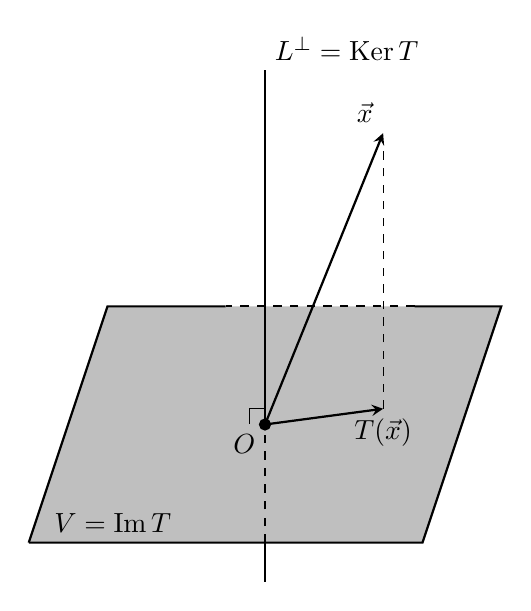
\begin{tikzpicture}
        \draw[fill=lightgray, draw=none] (0,0) -- (5,0) -- (6,3) -- (1, 3) -- cycle;
        \draw[thick] (0,0) -- (5,0) -- (6,3) -- (4.9, 3); % -- (1,4) -- cycle;
        \draw[thick,dashed] (4.9, 3) -- (2.5,3);
        \draw[thick] (2.5, 3) -- (1,3) -- (0,0);
        \node[anchor = south west] at (0.2, 0) {$V=\image T$}; 
        \filldraw (3,1.5) circle (2pt) node[anchor=north east]{$O$};
        \draw (3,1.5) -- (3,6) node[anchor=south west]{$L^{\perp} = \kernel{T}$};
        \draw[dashed] (3,0) -- (3,1.5);
        \draw (3,-0.5) -- (3,0);
        \draw (3, 1.7) -- (2.8, 1.7) -- (2.8, 1.5);
        \draw[thick, -stealth] (3, 1.5) -- (4.5, 5.2) node[anchor=south east]{$\vec{x}$};
        \draw[dashed] (4.5, 1.7) -- (4.5, 5);
        \draw[thick, -stealth] (3,1.5) -- (4.5, 1.7) node[anchor = north]{$T(\vec{x})$};
    \end{tikzpicture}
    \caption{Kernel and image of $T$.}
    \label{fig: orthogonal projection to plane for rnt}
\end{figure}

Take, for example, a linear transformation $T:\R^3 \to \R^3$ of an orthogonal projection onto a plane $V \subseteq \R^3$ with line $L^{\perp}$ being normal to $V$. This is going to be a conceptual example, so we won't use its matrix for any real calculations. See Figure \ref{fig: orthogonal projection to plane for rnt}. 

As seen, $\image{T}=V$, a two-dimensional linear subspace. Further, all vectors perpendicular to $V$, forming $L^{\perp}$, get mapped to $\vec{0}$ by $T$, i.e. $\kernel{T}=L^{\perp}$, a one-dimensional subspace. The domain of $T$ has three dimensions. We can verify that
\[\spacedim\R^3 = 3 = 1 + 2 = \spacedim\kernel{T} + \spacedim\image{T}.\]

We can think about the Rank-Nullity Theorem as some sort of "conservation" of dimensions. $\dim\kernel{T}$ counts the dimensions of $\R^3$ that ``collapse'' to $\vec{0}$ as we apply $T$, while $\dim\image{T}$ counts those that ``survive'' under $T$. Naturally, $\dim\kernel{T}$ and $\dim\image{T}$ should add up to $\dim\R^3$ in our example.


\chapter{Inverting Transformations}
\section{Properties of Functions}

\subsection{Identity and Inverse Functions}
\begin{definition}[identity function]
    \label{defn: identity function}
    Let $X$ be a set. We define the \textbf{identity function} $I_X: X \to X$ such that for all $x \in X$, $I_X(x)=x$.
\end{definition}

\begin{theorem}[Composition of function and identity function]
    \label{thm: composition of function and identity function}
    Let $X$ and $Y$ be sets, and let $f:X \to Y$. Then, $f=f \circ I_X = I_Y \circ f$.
\begin{proof}
    Pick any $x \in X$. Then, 
    \[\left(f\circ I_X \right)(x) = f\left(I_X\left(x\right)\right) = f(x)\]
    i.e. $f \circ I_X = f$. Also,
    \[\left(I_Y \circ f\right)(x) = I_Y\left(f(x)\right) = f(x)\]
    i.e. $I_Y \circ f = f$. 
\end{proof}
\end{theorem}

\begin{definition}[invertibility and inverse]
    \label{defn: invertibility and inverse}
    Let $X$ and $Y$ be sets, and $f:X \to Y$ be a function. We say $f$ is \textbf{invertible} if and only if there exists a function $\inv{f}: Y \to X$ (which we call the \textbf{inverse of $\pmb{f}$}) such that $\inv{f} \circ f = I_X$ and $f \circ \inv{f} = I_Y$.
\end{definition}

\begin{remark}
    Let $X$ and $Y$ be sets, and $f:X \to Y$ be an invertible function. By Definition \ref{defn: invertibility and inverse}, we have
    \begin{itemize}
        \item for all $a \in X$, $\inv{f} \left(f\left(a\right)\right) = \left(\inv{f} \circ f\right)(a) = I_x(a) = a$; and
        \item for all $b \in Y$, $f \left(\inv{f}\left(b\right)\right) = \left(f \circ \inv{f}\right)(b) = I_Y(b) = b$.
    \end{itemize}
\end{remark}

Theorem \ref{thm: uniqueness of inverse functions} discusses the uniqueness of inverse functions.
\begin{theorem}[Uniqueness of inverse functions]
    \label{thm: uniqueness of inverse functions}
    Let $X$ and $Y$ be sets, and let $f:X \to Y$ be an invertible function. Then, $\inv{f}:Y \to X$ is unique.
\begin{proof}
    Let $g:Y \to X$ and $h: Y \to X$ both be inverse functions of $f$. Since $g$ is an inverse function of $f$, by Definition \ref{defn: invertibility and inverse}, $g \circ f = I_X$ and $f \circ g = I_Y$. Similarly, $h \circ f = I_X$ and $f \circ h = I_Y$.
    
    By Theorem \ref{thm: composition of function and identity function}, $g = I_X \circ g$. Since $h \circ f = I_X$, it must be the case that $g = (h \circ f) \circ g$. Since function composition is associative, we have $g = h \circ (f \circ g)$. Since $g$ is an inverse function of $f$, by Definition \ref{defn: invertibility and inverse}, $f \circ g = I_Y$, i.e. $g = h \circ (f \circ g) = h \circ I_Y$. Again, by Theorem \ref{thm: composition of function and identity function}, we have
    \[g=h,\]
    i.e. we have shown that inverse functions are unique.
\end{proof}
\end{theorem}

\begin{theorem}[Invertibility implies unique solution]
    \label{thm: invertibility implies unique solution}
    Let $X$ and $Y$ be sets. Then, $f:X \to Y$ is invertible if and only if for all $y \in Y$, there exists a unique solution $x \in X$ such that $f(x)=y$.
\begin{proof}
    For the forward direction, suppose $f:X \to Y$ is invertible. Then, by definition, there exists function $\inv{f}:Y \to X$ such that $\inv{f} \circ f = I_X$ and $f \circ \inv{f} = I_Y$.
    
    Pick any $y \in Y$, and we have equation $f(x)=y$. Applying function $\inv{f}$ on both sides,
    \[\inv{f}(f(x)) = \inv{f}(y) \Longrightarrow (\inv{f} \circ f)(x) = \inv{f}(y).\]
    Since $\inv{f} \circ f = I_X$ and $I_X(x) = x$, we have
    \[x = \inv{f}(y).\]
    
    This is a unique solution, because $\inv{f}$ is a unique inverse function of $f$.
    
    For the backward direction, let $f:X \to Y$ be a function such that for all $y \in Y$, there exists a unique $x \in X$ such that $f(x)=y$. Then, we define function $S: Y \to X$ such that for all $y \in Y$, $S(y)$ is such a unique solution to $f(x)=y$. 
    
    Pick any $b \in Y$. Then, $S(b)$ is the unique $x \in X$ such that $f(x)=b$, i.e. $f(S(b)) = b$, i.e. $(f \circ S)(b) = b$. Hence $f \circ S = I_Y$.
    
    Pick any $a \in X$. Then, $S(f(a))$ is the unique $x \in X$ such that $f(x)=f(a)$. The solution to this equation is $x=a$, which is unique because of the assumption in this part. Therefore, $S(f(a)) = a$, i.e. $(S \circ f)(a) = a$. Hence $S \circ f = I_X$.
    
    Since $f \circ S = I_Y$ and $S \circ f = I_X$, $S = \inv{f}$, i.e. $f$ is invertible.
\end{proof}
\end{theorem}

\subsection{Surjectivity, Injectivity, and Invertibility}
\begin{definition}[surjectivity, onto]
    \label{defn: surjectivity, onto}
    Let $X$ and $Y$ be sets, and let $f:X \to Y$ be a function. We say $f$ is \textbf{surjective}, or \textbf{onto}, if and only if for all $y \in Y$, there exists $x \in X$ such that $f(x) = y$.
\end{definition}
\begin{remark}
    Saying that $f:X \to Y$ is surjective is equivalent to saying that for all $y \in Y$, $f(x)=y$ has at least one solution $x \in X$.
\end{remark}
\begin{remark}
    Function $f:X \to Y$ is surjective if and only if $\image f = Y$, the codomain.
\end{remark}
\begin{theorem}[Surjectivity and image]
    \label{thm: surjectivity and image}
    Let $X$ and $Y$ be sets, and let $f:X \to Y$ be a function. Then, $f$ is surjective if and only if $\image(f) = Y$.
\end{theorem}
\begin{definition}[injectivity, one-to-one]
    \label{defn: injectivity, one-to-one}
    Let $X$ and $Y$ be sets, and let $f: X \to Y$ be a function. We say that $f$ is \textbf{injective}, or \textbf{one-to-one}, if and only if for all $x_1, x_2 \in X$, $f(x_1) = f(x_2) \Longrightarrow x_1 = x_2$.
\end{definition}
\begin{remark}
    Saying that $f:X \to Y$ is injective is equivalent to saying that for all $y \in Y$, $f(x)=y$ has at most one solution $x \in X$.
\end{remark}

Recall that a function $f: X \to Y$ is invertible if and only if for all $y \in Y$, there exists a unique $x \in X$ such that $f(x)=y$, from Theorem \ref{thm: invertibility implies unique solution}. From the definitions above, we arrive at Theorem \ref{thm: invertibility, surjectivity, injectivity}.

\begin{theorem}[Invertibility, surjectivity, and injectivity]
    \label{thm: invertibility, surjectivity, injectivity}
    Let $f:X \to Y$ be a function for sets $X$ and $Y$. Then, $f$ is invertible if and only if $f$ is both surjective and injective.
\begin{proof}
    Suppose $f$ is invertible. Then, there exists a unique $x \in X$ such that $f(x)=y$ as shown in Theorem \ref{thm: invertibility implies unique solution}. The ``existence'' clause implies ``at least one'', i.e. $f$ is surjective. The ``unique'' clause implies ``at most one'', i.e. $f$ is injective. 
    
    Suppose $f$ is both injective and surjective. Since $f$ is surjective, there exists at least one solution $x \in X$ such that $f(x)=y$. Since $f$ is injective, there exists at most one solution $x \in X$ such that $f(x)=y$. Therefore, by Theorem \ref{thm: invertibility implies unique solution}, $f$ is invertible.
\end{proof}
\end{theorem}


\section{Properties of Linear Transformations as Functions}
Since a linear transformation is a function operating on vectors, we can apply the definitions of the properties of functions to linear transformations.
\subsection{Surjectivity}
Let $T:\R^n \to \R^m$ be a linear transformation with $m \times n$ matrix $\mat{A}$, i.e. $T(\vec{x}) = \mat{A}\vec{x}$. Let $\mat{A} = \cmat[a]$.

By definition, $T$ is onto if and only if for all $\vec{b} = \vecxxdx[b]$ there exists $\vec{x} = \vecxxdx$ such that $\mat{A}\vec{x} = \vec{b}$. Multiplying out $\mat{A}$ and $\vec{x}$ gives us \[\mat{A} \vec{x} = x_1\vec{a}_1 + x_2\vec{a}_2 + \cdots + x_n\vec{a}_n\]
which is nothing but a linear combination of the column vectors of $\mat{A}$. The set of all $\mat{A}\vec{x}$s, therefore, is just the span of the column vectors of $\mat{A}$, i.e. $C(\mat{A})$. This gives us our first hint: $T$ is onto if $C(\mat{A}) = \R^m$, i.e. the column vectors of $\mat{A}$ spans $\R^m$. This result makes sense because $C(\mat{A})$ is the set of all possible $\mat{A}\vec{x}$s. If there exists $\vec{y} \in \R^m$ that does not exist in $C(\mat{A})$, then for all $\vec{x} \in \R^n$, $T(\vec{x}) \neq \vec{y}$, i.e. $T$ is not surjective. 

If there exists $\vec{b} \in \R^m$ for which the system of equations represented by augmented matrix $\begin{bmatrix}[c|c]\mat{A} & \vec{b}\end{bmatrix}$ has no solution, then $T$ is not onto. 

When does the system of equations not have a solution? This case occurs when the row-reduced echelon form has a row like $\begin{bmatrix}[ccc|c]0 & \cdots & 0 & (\text{some nonzero value})\end{bmatrix}$. If, for some $\vec{b} \in \R^m$, $\rref\begin{bmatrix}[c|c]\mat{A} & \vec{b}\end{bmatrix}$ contains such a row, then this $\mat{A}\vec{x} = \vec{b}$ does not have a solution, i.e. $T$ is not onto.

A system of linear equations (represented by $T(\vec{x}) = \mat{A}\vec{x} = \vec{b}$) can only have either no solution, one solution, or infinitely many solutions. If $\rref\mat{A}$ contains a row of all zeroes, then either
\begin{itemize}
    \item $\rref\begin{bmatrix}[c|c]\mat{A} &\vec{b}\end{bmatrix}$ contains a row of all zeroes on one side and nonzero value on the other side for some $\vec{b} \in \R^m$. In this case, $T$ is not onto; or
    \item for all $\vec{b} \in \R^m$, $\rref\begin{bmatrix}[c|c]\mat{A} &\vec{b}\end{bmatrix}$ contains a row of all zeroes on both sides. This case is not possible because the right-side of this all-zero row must be of form of $k_1b_1 + k_2b_2 + \cdots + k_nb_n$ due to the nature of computing row-reduced echelon forms. There will be some choice of $\vec{b}$ that makes this entry nonzero.
\end{itemize}
Otherwise, if $\rref\mat{A}$ does not contain a row of all zeroes, then $\mat{A} \vec{x} = \vec{b}$ must have one or infinitely many solutions for all $\vec{b} \in \R^m$. Then, $T$ is onto.

We summarize this finding in Theorem \ref{thm: surjectivity of linear transformations}.
\begin{theorem}[Surjectivity of linear transformations]
    \label{thm: surjectivity of linear transformations}
    Let $T:\R^n \to \R^m$ be a linear transformation such that for all $\vec{x} \in \R^n$, $T(\vec{x}) = \mat{A}\vec{x}$ for $m \times n$ matrix $\mat{A}$. Then, $T$ is onto if and only if $C(\mat{A}) = \R^m$, if and only if $\rref{\mat{A}}$ does not contain a row of all zeroes, i.e. $\rref\mat{A}$ has a pivot in every row.
\end{theorem}

\begin{remark}
    Now recall Theorem \ref{thm:basis v pivot} which says that the corresponding columns in $\mat{A}$ of the pivot columns in $\rref\mat{A}$ form a basis for $C(\mat{A})$ for some matrix $\mat{A}$. Definition \ref{defn:dimensionality of subspace} tells us that $\spacedim C(\mat{A})$ is the number of basis vectors for $C(\mat{A})$. We also know that $\rank\mat{A}=\spacedim C(\mat{A})$ from Theorem \ref{thm: dimension v.s. rank}. 
    
    Statement ``$\rref\mat{A}$ has a pivot in every row'' is equivalent to $\rref\mat{A} = m$, since $\mat{A}$ has $m$ rows. Hence, $T$ is onto if and only if $\rank\mat{A} = m$.
\end{remark}

\subsection{Injectivity}
We start with a discussion about the solution set of a particular instance of $\mat{M}\vec{x}=\vec{b}$ in Example \ref{expl: solution set Ax=b}.
\begin{example}
    \label{expl: solution set Ax=b}
    Let $T: \R^2 \to \R^2$ be defined by $T\vecxx = \mat{M}\vecxx$ for $\mat{M} = \begin{bmatrix}1 & -3 \\ -1 & 3\end{bmatrix} $, and let $\vec{b} = \vecxx[b] \in \R^2$. Let us solve the equation $T(\vec{x}) = \vec{b}$, i.e. $ \begin{bmatrix}1 & -3 \\ -1 & 3\end{bmatrix} \vecxx = \vecxx[b]$. 
    
    We have augmented matrix $\mat{A} = \begin{bmatrix}[cc|c] 1 & -3 & b_1 \\ -1 & 3 & b_2 \end{bmatrix}$, and its row-reduced echelon form is \[\rref\mat{A} = \begin{bmatrix}[cc|c]1 & -3 & b_1 \\ 0 & 0 & b_1 + b_2\end{bmatrix}.\]
    
    At first glance, this equation only has solution when $b_1 + b_2 = 0$, i.e. $b_2 = -b_1$. Otherwise, we would have a row with all zeroes on one side and a nonzero number on the other side, leading to no solution. The image of $T$ is, then, all sets of $\vec{b} \in \R^2$ where $b_2 = -b_1$. Visualizing the image of $T$ on the codomain $b_1-b_2$--plane, we see that $\image{T}$ falls on a line with slope of $-1$ passing the origin. 

    Clearly, $T$ is not onto, since when, say, $\vec{b} = \colvec{2}{1}{1}$, $b_2 \neq b_1$, nothing from the domain maps to $\vec{b}$. From another perspective, since $\image{T} \neq \R^2$, $T$ is not onto.
    
    Now we focus on the $\vec{b}$s for which the equation does have solutions. In this case, the solution set is
    \[\vecxx = \colvec{2}{b_1}{0} + t\colvec{2}{3}{1}.\]
    
    We pick $\vec{b} = \vec{0}$. This equation has a solution ($0 = -0$) and the solution set is
    \[\vecxx = t\colvec{2}{3}{1}.\]
    Recall that the solution set for $\mat{M}\vec{x} = \vec{0}$ is the \textit{null space} of $\mat{M}$, i.e.$N(\mat{M}) = \left\{t\colvec{2}{3}{1} \suchthat t \in \R\right\}$.
    
    Now say $\vec{b} = \colvec{2}{5}{-5}$. This equation has a solution, and plugging it in, the solution set is
    \[\vecxx = \colvec{2}{5}{0} + t\colvec{2}{3}{1}.\]
    
    Now say $\vec{b} = \colvec{2}{-5}{5}$. This equation has a solution, and the solution set is
    \[\vecxx = \colvec{2}{-5}{0} + t\colvec{2}{3}{1}.\]

    Observe that when $\vec{b} = \colvec{2}{5}{-5}$ and when $\vec{b} = \colvec{2}{-5}{5}$, the solution set is nothing but the \textit{shifted} version of $N(\mat{M})$. Indeed, for any $\vec{b} = \vecxx[b]$ where $b_1 + b_2 = 0$, the solution set is $\left\{\colvec{2}{b_1}{0} + t\colvec{2}{3}{1} \suchthat t \in \R\right\}$. \hfill \qedsymbol
\end{example}

We generalizes the findings of Example \ref{expl: solution set Ax=b} in Theorem \ref{thm: solution set and null space}.
\begin{theorem}[Solution set and null space]
    \label{thm: solution set and null space}
    Let $T:\R^n \to \R^m$ be a linear transformation with $m \times n$ matrix $\mat{M}$. Assuming $T\left(\vec{x}\right) = \vec{b}$ has solution for some $\vec{b}$. Then, the solution set is $\left\{\vec{x}_p + \vec{n} \suchthat \vec{n} \in N(\mat{M})\right\}$ for some particular vector $\vec{x}_p$.
\begin{proof}
    Assume that $T(\vec{x}) = \vec{b}$ has solutions, and let $\vec{x}_p$ be a particular solution to the equation. 
    
    First, we show that for all $\vec{n} \in N(\mat{M})$, $\vec{x}_p + \vec{n}$ is a solution to $T(\vec{x}) = \vec{b}$. Pick any $\vec{n} \in N(\mat{M})$. 
    Since $\vec{x}_p$ is a solution to $\mat{M}\vec{x} = \vec{b}$, and since $\vec{n} \in N(\mat{M})$, it must be the case that
    \[T(\vec{x}_p + \vec{n}) = T(\vec{x}_p) + T(\vec{n}) = \mat{M}\vec{x}_p + \mat{M}\vec{n} = \vec{b} + \vec{0} = \vec{b}\] i.e. $\vec{x}_p + \vec{n}$ is a solution to equation $T(\vec{x}) = \vec{b}$.
    
    Second, we show that any solutions to $T(\vec{x}) = \vec{b}$ can be written as $\vec{x}_p + \vec{n}$ for some $\vec{n} \in N(\mat{M})$. Let $\vec{x}$ be a solution to $T(\vec{x}) = \vec{b}$. Then, we have
    \[T(\vec{x} - \vec{x}_p) = T(\vec{x}) - T(\vec{x}_p).\]
    Since $\vec{x}$ and $\vec{x}_p$ are both solutions to $T(\vec{x} )= \vec{b}$, we conclude that 
    \[T(\vec{x} - \vec{x}_p) = T(\vec{x}) - T(\vec{x}_p) = \vec{b} - \vec{b} = \vec{0}.\]
    Therefore, $\vec{x} - \vec{x}_p \in N(\mat{M})$. Since $\vec{x} = \vec{x}_p + (\vec{x} - \vec{x}_p)$ and $\vec{x} - \vec{x}_p \in N(\mat{M})$, any solutions to $T(\vec{x}) = \vec{b}$ can be written as $\vec{x}_p + \vec{n}$ for some $\vec{n} \in N(\mat{M})$.
\end{proof}
\end{theorem}

Now we can discuss about injectivity of a linear transformation $T:\R^n \to \R^m$ defined by $m \times n$ matrix $\mat{M}$. By definition of injectivity, $T(\vec{x}) = \vec{b}$ must have \textit{at most} one solution (possibly zero), i.e. the size of set $\left\{\vec{x}_p + \vec{n} \suchthat \vec{n} \in N(\mat{M})\right\}$ must be at most one, implying that $N(\mat{M})$ must have one element. Since $N(\mat{M})$ is a linear subspace, $\vec{0} \in N(\mat{M})$. Therefore, $N(\mat{M}) = \left\{\vec{0}\right\}$. Then, by Theorem \ref{thm:null space linear dependence}, the column vectors of $\mat{M}$ must be linearly independent. 

We know that $C(\mat{M})$ is the span of the column vectors of $\mat{M}$. Since the column vectors of $\mat{M}$ are linearly independent, the column vectors form a basis for $C(\mat{M})$, i.e. $\spacedim C(\mat{M}) = n$, i.e. $\rank\mat{M} = n$ by Theorem \ref{thm: dimension v.s. rank}.

To summarize, if $T$ is injective, then $N(\mat{M}) = \left\{\vec{0}\right\}$. Then, the column vectors of $\mat{M}$ are linearly independent. Then, the column vectors of $\mat{M}$ form a basis for $C(\mat{M})$. Then, $\spacedim C(\mat{M}) = \rank(\mat{M}) = n$. Conversely, if $\rank(\mat{M})=n$, then the column vectors of $\mat{M}$ form a basis for $C(\mat{M})$. Then, the column vectors of $\mat{M}$ are linearly independent. Then, $N(\mat{M}) = \left\{\vec{0}\right\}$. Then, $T$ is one-to-one. 

We formalize this finding in Theorem \ref{thm: injectivity, rank, and linear independence}.
\begin{theorem}[Injectivity, rank, and linear independence]
    \label{thm: injectivity, rank, and linear independence}
    Let $T(\vec{x}) = \mat{M}\vec{x}$ be a linear transformation, where $\mat{M}$ is a $m \times n$ matrix. Then, $T$ is injective if and only if $\rank\mat{M} = n$, if and only if the column vectors of $\mat{M}$ are linearly independent.
\end{theorem}

\subsection{Invertibility}
\label{section: invertibility of linear transformations}
Let $T:\R^n \to \R^m$ be a linear transformation with $m \times n$ matrix $\mat{M}$. Is $T$ invertible? 

By definition of invertibility (Definition \ref{defn: invertibility and inverse}), $T$ is invertible if and only if $T$ is both surjective and injective. 

By Theorem \ref{thm: surjectivity of linear transformations}, $T$ is surjective if and only if $\rank \mat{M} = m$. By Theorem \ref{thm: injectivity, rank, and linear independence}, $T$ is injective if and only if $\rank \mat{M} = n$. In order for $T$ to be both injective and surjective, then, $\rank \mat{M} = m = n$, which means $\mat{M}$ must be a square matrix (see Definition \ref{defn: square matrix}).

\begin{definition}[square matrix]
    \label{defn: square matrix}
    Let $\mat{M}$ be an $m \times n$ matrix. We say $\mat{M}$ is a \textbf{square matrix} if and only if $m = n$.
\end{definition}

Since $\rank \mat{M} = n$, every column of $\rref\mat{M}$ must be a pivot column that are linearly independent. By definition of pivot columns, then, $\rref \mat{M} = \idmat[n]$.

We summarize this result in Theorem \ref{thm: invertibility of linear transformations}.

\begin{theorem}[Invertibility of linear transformations]
    \label{thm: invertibility of linear transformations}
    Let $T: \R^n \to \R^m$ be a linear transformation with $m \times n$ matrix $\mat{M}$. Then, $T$ is invertible if and only if $m=n$ and $\rref\mat{M} = \idmat[n]$. 
\end{theorem}

Suppose $T: \R^n \to \R^n$ is an invertible linear transformation. Then, by Definition \ref{defn: invertibility and inverse}, there must exist some \textit{inverse transformation} $\inv{T}$ such that $\inv{T} \circ T = I_{\R^n}$ and $T \circ \inv{T} = I_{\R^n}$. We will show that $\inv{T}$ is a linear transformation in Theorem \ref{thm: inverses of linear transformations are linear}.

\begin{theorem}[Inverses of linear transformations are linear]
    \label{thm: inverses of linear transformations are linear}
    Let $T: \R^n \to \R^n$ be an invertible linear transformation. Then, $\inv{T}$ is linear.
\begin{proof}
    First, we show that for all $\vec{u},\vec{v} \in \R^n$, $\inv{T}\left(\vec{v} + \vec{v}\right) = \inv{T}\left(\vec{u}\right) + \inv{T}\left(\vec{v}\right)$.
    
    Pick any $\vec{u},\vec{v} \in \R^n$. We have
    \begin{align*}
        (T \circ \inv{T})(\vec{u} + \vec{v}) &= \vec{u} + \vec{v} & \because T \circ \inv{T} = I_{\R^n} \\
        &= (T \circ \inv{T})(\vec{u}) + (T \circ \inv{T})(\vec{v}) & \because T \circ \inv{T} = I_{\R^n} \\
        T(\inv{T}(\vec{u}+ \vec{v})) &= T(\inv{T}(\vec{u})) + T(\inv{T}(\vec{v})) \\
        &= T(\inv{T}(\vec{u}) + \inv{T}(\vec{v})) & \because \text{$T$ is linear} \\
        \inv{T}(\vec{u} + \vec{v}) &= \inv{T}(\vec{u}) + \inv{T}(\vec{v}). & \because \text{$T$ is injective}
    \end{align*}
    
    Now, we show that for all $\vec{v} \in \R^n, c \in \R$, $\inv{T}(c\vec{v}) = c\inv{T}(\vec{v})$.
    
    Pick any $\vec{v} \in \R^n$ and $c \in \R$. Then,
    \begin{align*}
        (T \circ \inv{T})(c\vec{v}) &= c\vec{v} & \because T \circ \inv{T} = I_{\R^n} \\
        &= c(T \circ \inv{T})(\vec{v}) & \because T \circ \inv{T} = I_{\R^n} \\
        T(\inv{T}(c\vec{v})) &= cT(\inv{T}(\vec{v})) \\
        &= T(c\inv{T}(\vec{v})) & \because \text{$T$ is linear} \\
        \inv{T}(c\vec{v}) &= c\inv{T}(\vec{v}). & \because \text{$T$ is injective}
    \end{align*}
\end{proof}
\end{theorem}

Since $\inv{T}$ is a linear transformation, by Theorem \ref{thm:lt=mvp}, there must be a matrix for $\inv{T}$, as defined in Definition \ref{defn: matrix inverse}.

\begin{definition}[invertibility and inverse of a matrix]
    \label{defn: matrix inverse}
    Let $\mat{M}$ be an $n \times n$ matrix, and $T(\vec{x}) = \mat{M}\vec{x}$ be an invertible linear transformation. We say that $\mat{M}$ is invertible. Then, we say $\invm{M}$ is the matrix of linear transformation $\inv{T}$, i.e. $\inv{T}(\vec{x}) = \invm{M}\vec{x}$. We call $\invm{M}$ as the \textbf{$\pmb{\mat{M}}$ inverse}.
\end{definition}

We will discuss a few important properties of $\invm{M}$. We know that \[(\inv{T} \circ T)(\vec{x}) = \invm{M} \mat{M} \vec{x}\] by definition of linear transformation composition. Since $\inv{T} \circ T = I_{\R^n}$, \[(\inv{T} \circ T)(\vec{x}) = \vec{x} = \idmat[n]\vec{x}.\] Therefore, \[\invm{M}\mat{M} = \idmat[n].\]

The other direction also holds, i.e. $\mat{M} \invm{M} = \idmat[n]$. We formalize this finding in Theorem \ref{thm: product between inverse matrix and original matrix}.

\begin{theorem}[Product between inverse matrix and original matrix]
    \label{thm: product between inverse matrix and original matrix}
    Let $\mat{M}$ be an invertible $n \times n$ matrix. Then, 
    \[\mat{M}\invm{M} = \invm{M}\mat{M} = \idmat[n].\]
    Let $\mat{A},\mat{B}$ be $n \times n$ matrices. Then,
    \[\mat{A}\mat{B} = \idmat[n]\]
    if and only if $\mat{A} = \invm{B}$ and $\mat{B} = \invm{A}$.
\end{theorem}

We demonstrate our findings above in Example \ref{expl: check matrix invertibility}.
\begin{example}
    \label{expl: check matrix invertibility}
    Let \[\mat{M} = \begin{bmatrix}1 & 1 & 1 \\ 1 & 2 & k \\ 1 & 4 & k^2\end{bmatrix}.\] For which values of $k$ does $\mat{M}$ have an inverse?
\begin{solution}
    We compute the row-reduced echelon form, taking notes of the assumptions made in the process.

    \[\begin{bmatrix}1 & 1 & 1 \\ 1 & 2 & k \\ 1 & 4 & k^2 \end{bmatrix} \rightsquigarrow \begin{bmatrix}\boxed{1} & 1 & 1 \\ 0 & 1 & k-1 \\ 0 & 3 & k^2 - 1\end{bmatrix} \rightsquigarrow \begin{bmatrix}\boxed{1} & 0 & 2-k \\ 0 & \boxed{1} & k-1 \\ 0 & 0 & k^2 - 3k + 2\end{bmatrix}\]
    Now we have to assume that $k^2-3k+2 \neq 0$ so we can divide the third row by $k^2 - 3k + 2$, and then subtract the first row by $(2-k)$ times the third row, and subtract the second row by $(k-1)$ times the third row, to yield
    \[\rightsquigarrow \begin{bmatrix}\boxed{1} & 0 & 0 \\ 0 & \boxed{1} & 0 \\ 0 & 0 & \boxed{1}\end{bmatrix}.\]

    Only by making the assumption that $k^2 - 3k + 2 \neq 0$ can we reach this $\idmat[3]$. Solving this inequality yields, $k \neq 1, 2$. Hence, this matrix is invertible if and only if $k \neq 1, 2$. \hfill \qedsymbol
\end{solution}
\end{example}

Now, as usual, we would like to study the properties of matrix transposes that apply to this section: invertibility. Let $\mat{A}$ be an invertible $n \times n$ matrix. Then, by Theorem \ref{thm: product between inverse matrix and original matrix}, $\mat{A}\invm{A}=\idmat$ and $\invm{A}\mat{A}=\idmat$. For the first equation, let's find the transposes of both sides. Given that $\idmat^T=\idmat$, and $\left(\mat{A}\invm{A}\right)^T = \left(\invm{A}\right)^T\mat{A}^T$ (from Theorem \ref{thm: transpose of matrix products}), we have equation
\[\left(\invm{A}\right)^T\mat{A}^T = \idmat.\]

Doing the same thing to the second equation, we have
\[\mat{A}^T\left(\invm{A}\right)^T = \idmat.\]

Therefore, by Theorem \ref{thm: product between inverse matrix and original matrix}, $\mat{A}^T$ and $\left(\invm{A}\right)^T$ are inverses of each other. 

We summarize this finding in Theorem \ref{thm: transposes of inverses}.

\begin{theorem}[Transposes of inverses]
    \label{thm: transposes of inverses}
    Let $\mat{A}$ be an invertible $n \times n$ matrix. Then, $\mat{A}^T$ and $\left(\invm{A}\right)^T$ are inverses of each other.
\end{theorem}

\begin{remark}
    A natural question to ask is: are the transposes of invertible matrices also invertible? The answer is yes, which we will show using determinants in Section \ref{section: determinants and invertibility}.
\end{remark}

Now, let $\mat{A} = \begin{bmatrix}\vert&\vert&&\vert \\ \vec{a}_1 & \vec{a}_2 & \cdots & \vec{a}_k \\ \vert & \vert & \vert & \vert \end{bmatrix}$ be an $n \times k$ matrix with column vectors $\vec{a}_1,\vec{a}_2,\cdots,\vec{a}_k$ being linear independent. Then, $\kernel\mat{A} = \left\{\vec{0}\right\}$ by Theorem \ref{thm:null space linear dependence}. Though we do not know whether $\mat{A}$ is invertible, we will now show that $\mat{A}^T\mat{A}$ is invertible. 

For $\mat{A}^T\mat{A}$ to be invertible, it must
\begin{itemize}
    \item be a square matrix. This is trivial to show: since $\mat{A}$ is $n \times k$ and $\mat{A}^T$ is $k \times n$, $\mat{A}^T\mat{A}$ is $k \times k$ and hence is square.
    \item have linearly independent column vectors, i.e. $\kernel\left(\mat{A}^T\mat{A}\right) = \left\{\vec{0}\right\}$. We can show this property by picking any $\vec{v} \in \kernel\left(\mat{A}^T\mat{A}\right)$ and deriving that $\vec{v} = \vec{0}$. 
    
    Pick any $\vec{v} \in \kernel\left(\mat{A}^T\mat{A}\right)$. Then, $\mat{A}^T\mat{A}\vec{x} = \vec{0}$. We multiply both sides of this equation by $\vec{v}^T$ to yield $\vec{v}^T\mat{A}^T\mat{A}\vec{x} = \vec{v}^T\vec{0}$. Since $\vec{v}^T\vec{0} = 0$, we have \[\vec{v}^T\mat{A}^T\mat{A}\vec{v} = 0.\]
    Since matrix products are associative (treating $\vec{v}$ as a matrix here), we have
    \[\left(\vec{v}^T\mat{A}^T\right)\left(\mat{A}\vec{v}\right) = 0.\]
    Since $\vec{v}^T\mat{A}^T = \left(\mat{A}\vec{v}\right)^T$ (see Theorem \ref{thm: transpose of matrix products}), we have
    \[\left(\mat{A}\vec{v}\right)^T\left(\mat{A}\vec{v}\right)=0.\]
    
    Let's do a quick sanity check here. We know $\vec{v} \in \R^k$ and $\mat{A}$ is $n \times k$. Hence, $\mat{A}\vec{v}$ is an $n \times 1$ column vector. Meanwhile, $\left(\mat{A}\vec{v}\right)^T$ is an $1 \times n$ row vector. Hence, by Theorem \ref{thm: vector transpose and dot product}, $\left(\mat{A}\vec{v}\right)^T\left(\mat{A}\vec{v}\right) = \left(\mat{A}\vec{v}\right)\cdot\left(\mat{A}\vec{v}\right)$. Then,
    $\left(\mat{A}\vec{v}\right)\cdot\left(\mat{A}\vec{v}\right) = 0$
    which tells us that \[\left\|\mat{A}\vec{v}\right\| = 0\] by definition of dot products. This only occurs when $\mat{A}\vec{v} = \vec{0}$, i.e. $\vec{v} \in \kernel\mat{A}$. 
    
    Since $\kernel\mat{A}=\left\{\vec{0}\right\}$, it must be the case that $\vec{v} = 0$.
\end{itemize}

We summarize this finding in Theorem \ref{thm: A-transpose x A is invertible}.
\begin{theorem}[$\mat{A}^T\mat{A}$ is invertible]
    \label{thm: A-transpose x A is invertible}
    Let $\mat{A}$ be a matrix with linearly independent columns. Then,
    $\mat{A}^T\mat{A}$ is invertible.
\end{theorem}

In Section \ref{section: finding inverse transformations} we will learn a more systematic way of telling whether a matrix is invertible by systematically finding the inverse matrices.

\section{Finding Inverse Transformations}
\label{section: finding inverse transformations}
The previous sections of this chapter tells us how to determine whether a matrix, and therefore a linear transformation, is invertible. However, most of the time, we actually want to find the inverse transformations given invertibility. Section \ref{section: general algorithm for finding inverse transformations and matrices} will show an general algorithm for determining whether a matrix is invertible, and if so, finding the inverse matrix, while in Section \ref{section: finding inverse transformations: special case for 2x2}, we will use this general algorithm to find a formula for the inverse of a $2 \times 2$ matrix, if it exists. Hopefully, Section \ref{section: finding inverse transformations: special case for 2x2} will lead naturally to Section \ref{section: determinants and invertibility}, where we will study the concepts of determinants.

\subsection{General Algorithm for Finding Inverse Transformations and Matrices}
\label{section: general algorithm for finding inverse transformations and matrices}
Say we have linear transformation $T_0(\vec{x}) = \mat{A}\vec{x}$ for $\mat{A} = \begin{bmatrix} 1 & -1 & -1 \\ -1 & 2 & 3 \\ 1 & 1 & 4\end{bmatrix}$, and we want to find $\rref\mat{A}$. For reasons made obvious later, we want to keep a record of what happened in each step of finding $\rref\mat{A}$.
\begin{align*}
    \mat{A} &= \begin{bmatrix} 1 & -1 & -1 \\ -1 & 2 & 3 \\ 1 & 1 & 4\end{bmatrix} \\
    &\rightsquigarrow \begin{bmatrix} 1 & -1 & -1 \\ 0 & 1 & 2 \\ 0 & 2 & 5 \end{bmatrix}& \begin{minipage}{0.4\linewidth}
    \begin{center}
        \textbf{Step 1}:
        \begin{varwidth}{\linewidth}
        $R2 \rightarrow R2 + R1$ \\
        $R3 \rightarrow R3 - R1$
        \end{varwidth}
    \end{center}
    \end{minipage} \\
    &\rightsquigarrow \begin{bmatrix} 1 & 0 & 1 \\ 0 & 1 & 2 \\ 0 & 0 & 1 \end{bmatrix}& \begin{minipage}{0.4\linewidth}
    \begin{center}
        \textbf{Step 2}: 
        \begin{varwidth}{\linewidth}
        $R1 \rightarrow R1 + R2$ \\
        $R3 \rightarrow R3 - 2\times R2$
        \end{varwidth}
    \end{center}
    \end{minipage} \\
    &\rightsquigarrow \begin{bmatrix} 1 & 0 & 0 \\ 0 & 1 & 0 \\ 0 & 0 & 1 \end{bmatrix} = \rref\mat{A}& \begin{minipage}{0.4\linewidth}
    \begin{center}
        \textbf{Step 3}: 
        \begin{varwidth}{\linewidth}
        $R1 \rightarrow R1 - R3$ \\
        $R2 \rightarrow R2 - 2\times R3$
        \end{varwidth}
    \end{center}
    \end{minipage}
\end{align*}

Now, each of the steps in finding $\rref\mat{A}$, which are just elementary row operations, is a linear transformation on the column vectors of the matrix. For instance, step 1 is equivalent to $T_1: \vecxxx[a] \mapsto \colvec{3}{a_1}{a_2 + a_1}{a_3-a_1}$. Then, if we apply this transformation to our standard basis vectors for $\R^3$, we find that the matrix for $T_1$ is \[\mat{S}_1 = \begin{bmatrix}1 & 0 & 0 \\ 1 & 1 & 0 \\ -1 & 0 & 1\end{bmatrix},\] i.e. $T_1(\vec{x}) = \mat{S}_1 \vec{x}$.

When we applied $T_1$ to our standard basis vectors and combined them into $\mat{S}$, we are essentially performing the same row operations onto $\idmat[3]$ that we performed to column vectors of $\mat{A}$. If we apply this transformation to each column of $\mat{A}$, forming a new matrix, we have
\[\begin{bmatrix}\vert & \vert & \vert \\  \mat{S}_1\colvec{3}{1}{-1}{1} & \mat{S}_1\colvec{3}{-1}{2}{1} & \mat{S}_1\colvec{3}{-1}{3}{4} \\ \vert & \vert & \vert \end{bmatrix}\]
which is nothing but $\mat{S}_1 \mat{A}$. Hence, running the first step of computing $\rref\mat{A}$ is equivalent to computing $\mat{S}_1 \mat{A}$.

Similarly, step 2 of the computation of $\rref \mat{A}$ involves another matrix $\mat{S}_2$ representing linear transformation $T_2$. Running step 2 of the computation is equivalent to computing product $\mat{S}_2 (\text{result from step 1}) = \mat{S}_2 \mat{S}_1 \mat{A}$.

Let $\mat{S}_3$ represent the third step of computation of $\rref\mat{A}$. In our case, the result after running step 3 is $\rref \mat{A}$, while running step 3 is equivalent to finding product $\mat{S}_3 (\text{result from step 2}) = \mat{S}_3\mat{S}_2\mat{S}_1\mat{A}$, i.e. $\rref{A} = \mat{S}_3\mat{S}_2\mat{S}_1\mat{A}$. 

With this knowledge, we can start finding the inverse of $\mat{A}$. Observe that $\rref\mat{A} = \idmat[3]$, so by Theorem \ref{thm: invertibility of linear transformations}, $\mat{A}$ is invertible. Since $\rref \mat{A} = \mat{S}_3\mat{S}_2\mat{S}_1\mat{A}$ and $\rref\mat{A} = \idmat[3]$, we know that
\[\mat{S}_3\mat{S}_2\mat{S}_1\mat{A} = \idmat[3].\]
Since matrix multiplication is associative (Theorem \ref{thm: matrix product associative and distributive properties}),
\[(\mat{S}_3\mat{S}_2\mat{S}_1)\mat{A} = \idmat[3].\]
By Theorem \ref{thm: product between inverse matrix and original matrix}, then, $\mat{S}_3\mat{S}_2\mat{S}_1 = \invm{A}$.

This is already some very exciting news, but it will get even better. Let's take the products $\mat{S}_3\mat{S}_2\mat{S}_1\mat{A}$ and $\mat{S}_3\mat{S}_2\mat{S}_1\idmat[3]$ side-by-side:
\begin{center}
    \begin{tabular}{c|c}
    $\mat{A}$ & $\idmat[3]$ \\
    $\mat{S}_1\mat{A}$ & $\mat{S}_1\idmat[3]$ \\
    $\mat{S}_2\mat{S}_1\mat{A}$ & $\mat{S}_2\mat{S}_1\idmat[3]$ \\
    $\mat{S}_3\mat{S}_2\mat{S}_1\mat{A}$ & $\mat{S}_3\mat{S}_2\mat{S}_1\idmat[3]$
\end{tabular}
\end{center}

The left side of the table is nothing but taking $\rref\mat{A}$. The right-side of the table is nothing but taking the same row-operations (represented by matrix products) with the identity matrix. Even better, $\mat{S}_3\mat{S}_2\mat{S}_1\idmat[3] = \mat{S}_3\mat{S}_2\mat{S}_1$. We took the same row-operations with the right-side as the left side to get $\rref\mat{A}$, and we get $\mat{S}_3\mat{S}_2\mat{S}_1$, which, as we computed before, is $\invm{A}$. Putting $\mat{A}$ and $\mat{I}$ side-by-side, solving for $\rref\mat{A}$, and applying the same row-operations to $\idmat[3]$, and we have found the inverse, if it exists!
We now have an algorithm of finding inverse matrices, if they exist. We summarize this finding in Theorem \ref{thm: algorithm for finding inverse}.

\begin{theorem}[An algorithm for finding inverse matrix]
    \label{thm: algorithm for finding inverse}
    Let $\mat{A}$ be an $n \times n$ matrix. To find $\invm{A}$, form the $n \times 2n$ matrix $\begin{bmatrix}[c|c]\mat{A} & \idmat[n]\end{bmatrix}$, and compute $\rref \begin{bmatrix}[c|c]\mat{A} & \idmat[n]\end{bmatrix} = \begin{bmatrix}[c|c]\mat{C} & \mat{D}\end{bmatrix}$. 
    \begin{itemize}
        \item If $\mat{C} = \idmat[n]$, then $\mat{D} = \invm{A}$.
        \item Otherwise, $\mat{A}$ is not invertible.
    \end{itemize}
\end{theorem}

\begin{example}
    \label{expl: finding inverse}
    Complete the process of finding the inverse of $\mat{A}$ as defined in the beginning of this section.
\begin{solution}
    We construct matrix 
    \[\begin{bmatrix}[ccc|ccc]1 & -1 & -1 & 1 & 0 & 0 \\ -1 & 2 & 3 & 0 & 1 & 0 \\ 1 & 1 & 4 & 0 & 0 & 1\end{bmatrix}.\]
    
    We have
    \[\rref \begin{bmatrix}[ccc|ccc]1 & -1 & -1 & 1 & 0 & 0 \\ -1 & 2 & 3 & 0 & 1 & 0 \\ 1 & 1 & 4 & 0 & 0 & 1\end{bmatrix} = \begin{bmatrix}[ccc|ccc] 1 & 0 & 0 & 5 & 3 & -1 \\ 0 & 1 & 0 & 7 & 5 & -2 \\ 0 & 0 & 1 & -3 & -2 & 1\end{bmatrix}.\]
    Since the left side of the row-reduced echelon form is the identity matrix, $\mat{A}$ is invertible. Hence, \[\invm{A}=\begin{bmatrix}5 & 3 & -1 \\ 7 & 5 & -2 \\ -3 & -2 & 1\end{bmatrix}.\] \hfill \qedsymbol
\end{solution}
\end{example}

\begin{example}
    Compute $\inv{\left(\invm{A}\right)}$ using techniques in Theorem \ref{thm: algorithm for finding inverse}. Verify that $\inv{\left(\invm{A}\right)} = \mat{A}$.
\begin{solution}
    We set up matrix
    \[\begin{bmatrix}[c|c] \invm{A} & \idmat[3] \end{bmatrix} = \begin{bmatrix}[ccc|ccc]5 & 3 & -1 & 1 & 0 & 0 \\ 7 & 5 & -2 & 0 & 1 & 0 \\ -3 & -2 & 1 & 0 & 0 & 1\end{bmatrix}.\]
    
    We have
    \[\rref{\begin{bmatrix}[c|c] \invm{A} & \idmat[3] \end{bmatrix}} = \begin{bmatrix}[ccc|ccc] 1 & 0 & 0 & 1 & -1 & -1 \\ 0 & 1 & 0 & -1 & 2 & 3 \\ 0 & 0 & 1 & 1 & 1 & 4\end{bmatrix}.\]
    
    Hence $\inv{\left(\invm{A}\right)} = \begin{bmatrix} 1 & -1 & -1 \\ -1 & 2 & 3 \\ 1 & 1 & 4\end{bmatrix} = \mat{A}$. \hfill \qedsymbol
\end{solution}
\end{example}

\subsection{Special Case for 2-by-2 Matrices}
\label{section: finding inverse transformations: special case for 2x2}

Let $\mat{A} = \begin{bmatrix} a & b \\ c & d\end{bmatrix}$. We want to find $\invm{A}$, if it exists. 


We construct matrix 
\[\mat{M} = \begin{bmatrix}[c|c] \mat{A} & \idmat[2] \end{bmatrix}_0 = \begin{bmatrix}[cc|cc] a & b & 1 & 0 \\ c & d & 0 & 1 \end{bmatrix}\] and want to compute $\rref\mat{M}$. It doesn't surprise us that if $a=c=0$, or if $b=d=0$, the left side of $\rref\mat{M}$ will never be the identity matrix, so $\mat{A}$ won't be invertible. Let's assume that $a \neq 0$ and $d \neq 0$. This way, at least one of $a,c$ will be nonzero, and at least one of $b,d$ will be nonzero. However, if $a = d = 0$ but $b,c \neq 0$, we can just flip the two rows of $\mat{M}$ to make $a,d \neq 0$. Then, we can start taking $\rref\mat{M}$, as follows.
\[\begin{bmatrix}[cc|cc] a & b & 1 & 0 \\ c & d & 0 & 1 \end{bmatrix} \rightsquigarrow \begin{bmatrix}[cc|cc]\boxed{1} & \frac{b}{a} & \frac{1}{a} & 0 \\ 0 & \frac{ad-bc}{a} & -\frac{c}{a} & 1\end{bmatrix}.\]

Now, to make the $\frac{ad-bc}{a}$ in the second row into $1$, we must assume $ad-bc \neq 0$ and divide by $\frac{ad - bc}{a}$. If $ad-bc = 0$, then this matrix is already in row-reduced echelon form, and the left side of $\rref\mat{M}$ will not be $\idmat[2]$, i.e. the matrix is not invertible. Dividing the second row by $\frac{ad - bc}{a}$ and replacing the first row with the first row minus $\frac{b}{a}$ times the second row, we have
\[\begin{bmatrix}[cc|cc]\boxed{1} & \frac{b}{a} & \frac{1}{a} & 0 \\ 0 & \frac{ad-bc}{a} & -\frac{c}{a} & 1\end{bmatrix} \rightsquigarrow \begin{bmatrix}[cc|cc]\boxed{1} & 0 & \frac{d}{ad-bc} & \frac{-b}{ad-bc} \\ 0 & \boxed{1} & \frac{-c}{ad-bc} & \frac{a}{ad-bc}\end{bmatrix} = \rref\mat{M}.\]

Therefore, \[\invm{A} = \begin{bmatrix}\frac{d}{ad-bc} & \frac{-b}{ad-bc} \\ \frac{-c}{ad-bc} & \frac{a}{ad-bc} \end{bmatrix} = \frac{1}{ad-bc} \begin{bmatrix}d & -b \\ -c & a \end{bmatrix}.\]

Recall that if $a=c=0$ or $b=d=0$, then we would have no inverses. Otherwise, inverses should exist. From the equation derived, we also see that if $ad-bc = 0$, we would be dividing by zero. Since $a=c=0$ or $b=d=0$ automatically leads to $ad-bc=0$, we can say that $\mat{A}$ has no inverses if and only if $ad-bc = 0$. 

To summarize, let $\mat{A} = \begin{bmatrix}a&b\\c&d\end{bmatrix}$. Then, $\mat{A}$ is invertable if and only if $ad - bc \neq 0$. If so, $\invm{A} = \frac{1}{ad-bc} \begin{bmatrix}d & -b \\ -c & a \end{bmatrix}$. The value of $ad - bc$ is interesting, because it determines whether $\mat{A}$ has an inverse. We will discuss more about this number in Section \ref{section: determinants and invertibility}.

\begin{example}
    If possible, find $\begin{bmatrix} 1 & 2 \\ 3 & 4 \end{bmatrix}^{-1}$.
\begin{solution}
    We have $(a,b,c,d) = (1,2,3,4)$. Since $ad-bc = 4-6 = -2 \neq 0$, the matrix is invertible. Hence,
    \[\begin{bmatrix} 1 & 2 \\ 3 & 4 \end{bmatrix}^{-1} = \frac{1}{ad-bc} \begin{bmatrix}d & -b \\ -c & a \end{bmatrix} = \begin{bmatrix}-2 & 1 \\ 3/2 & -1/3\end{bmatrix}.\]\hfill \qedsymbol
\end{solution}
\end{example}

\section{Determinants and Invertibility}
\label{section: determinants and invertibility}

In Definition \ref{defn: 2x2 determinant}, we will define the determinant for a $2 \times 2$ matrix. Later, in Definition \ref{defn: nxn determinant}, we will provide a recursive definition for an $n \times n$ matrix, $n \geq 3$.
\begin{definition}[determinant of a $2 \times 2$ matrix]
    \label{defn: 2x2 determinant}
    Let $\mat{A} = \begin{bmatrix}a & b \\ c & d \end{bmatrix}$. Then, we define the \textbf{determinant} of $\mat{A}$ to be \[\det\mat{A} = \begin{vmatrix}a & b \\ c & d\end{vmatrix} = ad-bc.\]
\end{definition}

We can now restate the findings in Section \ref{section: finding inverse transformations: special case for 2x2} for a $2 \times 2$ matrix.

\begin{theorem}[Formula for inverse of $2 \times 2$ matrix]
    \label{thm: formula for 2x2 inverse}
    Let $\mat{A} = \begin{bmatrix}a & b \\ c & d \end{bmatrix}$. If $\det\mat{A} = 0$, then $\mat{A}$ is not invertible. Otherwise, 
    \[\invm{A} = \frac{1}{\det\mat{A}}\begin{bmatrix}d & -b \\ -c & a\end{bmatrix}.\]
\end{theorem}

\begin{example}
    \label{expl: 2x2 inverse using determinant 2}
    Find $\begin{vmatrix} 1 & 2 \\ 3 & 6 \end{vmatrix}$, and if possible, find $\begin{bmatrix} 1 & 2 \\ 3 & 6 \end{bmatrix}^{-1}$.
\begin{solution}
    By Definition \ref{defn: 2x2 determinant}, we have
    \[\begin{vmatrix} 1 & 2 \\ 3 & 6 \end{vmatrix} = 1 \times 6 - 3 \times 2 = 0.\]
    Therefore, the matrix is not invertible.
    \hfill \qedsymbol
\end{solution}
\end{example}

We have been focusing on cases of $2 \times 2$ matrices. Let's extend this idea to multiple dimensions. Let $\mat{A}$ be an $n \times n$ matrix. Then, let $\mat{A}_{ij}$ be a $(n-1) \times (n-1)$ matrix we get if we `omit' the $i$-th row and the $j$-th column of $\mat{A}$. For example, say $\mat{B}=\begin{bmatrix} 1 & 2 & 3 \\ 4 & 5 & 6 \\ 7 & 8 & 9 \end{bmatrix}$. Then, $\mat{B}_{12} = \begin{bmatrix}4 & 6 \\ 7 & 9\end{bmatrix}$.

With $\mat{A}_{ij}$ defined, we can now provide one definition for the determinant of an $n \times n$ matrix, in Definition \ref{defn: nxn determinant}.

\begin{definition}[Laplace expansion]
    \label{defn: laplace expansion}
    \label{defn: nxn determinant}
    Let $\mat{A} = \elemmatnn$. Then,
    \[\det\mat{A} = a_{11}\det\mat{A}_{11} - a_{12}\det\mat{A}_{12} + a_{13}\det\mat{A}_{13} - \cdots \pm a_{1n}\det\mat{A}_{1n},\]
    where, for the sake of completeness of the theorem, $\mat{A}_{ij}$ is a $(n-1) \times (n-1)$ matrix we get by omitting the $i$-th row and $j$-th column of $\mat{A}$. We also say that $\det\mat{A}_{ij}$ is a \emph{minor} of $\mat{A}$.
    
    The algorithm of computing the determinant of a matrix using this definition of determinants is called \textbf{Laplace expansion}.
\end{definition}

\begin{remark}
    Note that Definitions \ref{defn: 2x2 determinant} and \ref{defn: nxn determinant} form a \textit{recursive} definition of determinant. A canonical algorithm implementing Laplace expansion has recursive runtime complexity of
    \[T(n) = nT(n-1) + n\] where $T(n)$ is the time it takes to compute the determinant of an $n \times n$ matrix. We can solve the recurrence relation to get that $T(n) \in O(n!)$. This is a very inefficient method of computing determinants, only suitable for smaller matrices. We will dedicate a part of Section \ref{section: properties of determinants} to exploring finding determinants by row-reduction.
\end{remark}

\begin{remark}
    We can, of course, define the determinant of an $1 \times 1$ matrix $\mat{M}=\begin{bmatrix}m\end{bmatrix}$ as $\det\mat{M}=m$. Then, we can recursively define the determinant of a $2 \times 2$ matrix using the determinant of an $1 \times 1$ matrix. Things should still work out the same.
\end{remark}


\begin{example}
    \label{expl: finding determinant for 4x4 matrix}
    Let $\mat{A} = \begin{bmatrix}1 & 2 & 3 & 4 \\ 1 & 0 & 2 & 0  \\ 0 & 1 & 2 & 3 \\ 2 & 3 & 0 & 0\end{bmatrix}$. Find $\det\mat{A}$.
\begin{solution}
    Using Definition \ref{defn: nxn determinant}, we have
    \[\det\mat{A} = 
    1\begin{vmatrix}0 & 2 & 0 \\ 1 & 2 & 3 \\ 3 & 0 & 0\end{vmatrix}
    - 2\begin{vmatrix}1 & 2 & 0 \\ 0 & 2 & 3 \\ 2 & 0 & 0\end{vmatrix}
    +3 \begin{vmatrix}1 & 0 & 0 \\ 0 & 1 & 3 \\ 2 & 3 & 0\end{vmatrix}
    - 4\begin{vmatrix} 1 & 0 & 2 \\ 0 & 1 & 2 \\ 2 & 3 & 0\end{vmatrix}.\]
    Now,
    \begin{align*}
        \begin{vmatrix}0 & 2 & 0 \\ 1 & 2 & 3 \\ 3 & 0 & 0\end{vmatrix} &= 0\times(\cdots) - 2\begin{vmatrix}1 & 3 \\ 3 & 0\end{vmatrix} + 0\times(\cdots) \\
        &= -2 \times (1 \times 0 - 3 \times 3) \\
        &= 18; \\
        \begin{vmatrix}1 & 2 & 0 \\ 0 & 2 & 3 \\ 2 & 0 & 0\end{vmatrix} &= 1 \times (2 \times 0 - 3 \times 0) - 2 \times (0 \times 0 - 2 \times 3) + 0 \times (\cdots) \\
        &= 12; \\
        \begin{vmatrix}1 & 0 & 0 \\ 0 & 1 & 3 \\ 2 & 3 & 0\end{vmatrix} &= 1 \times (1 \times 0 - 3 \times 3) - 0 \times (\cdots) + 0 \times (\cdots) \\
        &= -9; \text{ and}\\
        \begin{vmatrix} 1 & 0 & 2 \\ 0 & 1 & 2 \\ 2 & 3 & 0\end{vmatrix} &= 1 \times (1 \times 0 - 2 \times 3) - 0 \times (\cdots) + 2 \times (0 \times 3 - 1 \times 2) \\
        &= -10.
    \end{align*}
    Hence \[\det\mat{A} = 1(18) - 2(12) + 3(-9) - 4(-10) = 7.\] \hfill \qedsymbol
        
\end{solution}
\end{example}

Now, with the determinant of an $n \times n$ matrix defined, we can still use determinants to determine whether an arbitrary $n \times n$ matrix is invertible, just as we did in Section \ref{section: finding inverse transformations: special case for 2x2}. See Theorem \ref{thm: nxn matrix invertibility}.

\begin{theorem}[Invertibility of $n \times n$ matrices]
    \label{thm: nxn matrix invertibility}
    Let $\mat{A}$ be an $n \times n$ matrix. Then, $\mat{A}$ is invertible if and only if $\det\mat{A} \neq 0$.

\end{theorem}

\begin{intuition}
    Recall the determinant of a quadratic equation. Namely, if $ax^2 + bx + c=0$, then we say $b^2-4ac$ is the determinant, as the value of $b^2-4ac$ \emph{determines} the number of solutions the equation has. The determinants of matrices work similarly - they tell us whether matrices are invertible.
\end{intuition}

We have now been given the precise definitions of matrix determinants and a canonical and inefficient algorithm for computing determinants. The following subsections are dedicated to alternative and (perhaps) more efficient ways to compute determinants using their properties, as well as geometric understanding of determinants.

\subsection{Tricks for finding determinants}
Recall that in Definition \ref{defn: nxn determinant} and Example \ref{expl: finding determinant for 4x4 matrix}, we picked the first row $(a_{11}, \cdots, a_{1n})$, and for each entry in the first row $a_{1j}$, we computed $a_{1j} \det\mat{A}_{1j}$, where $\mat{A}_{ij}$ is matrix $\mat{A}$ except ignoring the $i$-th row and the $j$-th column. In actuality, we can compute the determinant the same way on different rows, and even columns. This technique becomes handy when a row or a column has a large number of zeroes, simplifying our calculation. 

Again, recall that in Definition \ref{defn: nxn determinant}'s formula for the determinant of an $n \times n$ matrix, the signs of each entry flip-flops as we progress from left to right in the first row. For instance, the sign used for the term representing $a_{11}\det\mat{A}_{11}$ is positive, while the sign used for term representing $a_{12}\det\mat{A}_{12}$ is negative, and the pattern continues. It turns out that going down from one row to the next when computing the determinant alternatively, we also encounter this pattern. Term representing $a_{11}\det\mat{A}_{11}$ is positive, while term representing $a_{21}\det\mat{A}_{21}$ is negative. 

Let us use this technique in Example \ref{expl: finding determinant for 4x4 matrix along other rows and columns}.

\begin{example}
    \label{expl: finding determinant for 4x4 matrix along other rows and columns}
    Compute $\det\mat{A}$ for $\mat{A}$ defined in Example \ref{expl: finding determinant for 4x4 matrix} using different rows and / or columns as seemed fit here.
\begin{solution}
    We first create a matrix of the signs representing each row and column.
    \[\mat{S}_4 = \begin{bmatrix}+&-&+&- \\ -&+&-&+ \\+&-&+&- \\ -&+&-&+\end{bmatrix}.\]
    The $i$-th row, $j$-th column of $\mat{S}_4$, denoted $s_{4,ij}$, is defined as such: $s_{4,ij} = (-1)^{i + j}$. 
    
    Notice that the fourth row of $\mat{A}$ has the most number of zeroes, which we want. Therefore, we have
    \begin{align*}
        \det\mat{A} &= s_{4,41}a_{41}\det\mat{A}_{41} + s_{4,42}a_{42}\det\mat{A}_{42} + s_{4,43}a_{43}\det\mat{A}_{43} + s_{4,44}a_{44}\det\mat{A}_{44} \\
        &= -2 \det\underbrace{\begin{bmatrix}2 & 3 & 4 \\ 0 & 2 & 0 \\ 1 & 2 & 3\end{bmatrix}}_{\mat{B}}  + 3 \det\underbrace{\begin{bmatrix}1 & 3 & 4 \\ 1 & 2 & 0 \\ 0 & 2 & 3 \end{bmatrix}}_{\mat{C}}.
    \end{align*}
    We omit the last two terms, because $a_{43} = a_{44} = 0$ and will not change the result. How do we find $\det\mat{B}$ and $\det\mat{C}$? We employ the same technique, creating
    \[S_3 = \begin{bmatrix}+ & - & + \\ - & + & - \\ + & - & +\end{bmatrix}\] where the $i$-th row, $j$-th column is given by $s_{3, ij} = (-1)^{i + j}$. For $\det\mat{B}$, at one glance, the second row seems to have two zeroes, which is beneficial to our computation. Therefore,
    \[\det\mat{B} = 2\det\begin{bmatrix}2 & 4 \\ 1 & 3\end{bmatrix} = 4.\]
    
    For $\det\mat{C}$, for the sake of demonstration, we will choose the first column, i.e.
    \[\det\mat{C} = 1 \det\begin{bmatrix}2 & 0 \\ 2 & 3\end{bmatrix} - 1 \det\begin{bmatrix}3 & 4 \\ 2 & 3\end{bmatrix} = 5.\]
    
    Hence,
    \[\det\mat{A} = -2\det\mat{B} +3\det\mat{C} = -2(4) + 3(5) = 7.\]
    \hfill \qedsymbol
\end{solution}
\end{example}

Now we will introduce another theorem that provides a closed formula for finding determinants of $3 \times 3$ matrices in Theorem \ref{thm: rule of sarrus}.

\begin{theorem}[Rule of Sarrus]
    \label{thm: rule of sarrus}
    Let $\mat{A} = \begin{bmatrix} a & b & c \\ d & e & f \\ g & h & i \end{bmatrix}$. Then, \[\det\mat{A} = aei + bgf + cdf - afh - bdi - ceg.\]
\begin{proof}
    \begin{align*}
        \begin{vmatrix} a & b & c \\ d & e & f \\ g & h & i \end{vmatrix} &= a\begin{vmatrix}e & f \\ h & i \end{vmatrix} - b\begin{vmatrix}d & f \\ g & i\end{vmatrix} + c\begin{vmatrix} d & e \\ g & h \end{vmatrix} \\
        &= a(ei - fh) - b(di - fg) + c(dh - eg) \\
        &= aei - afh - bdi + bfg + cdh - ceg \\
        &= aei + bgf + cdh - afh - bdi - ceg.
    \end{align*}
\end{proof}
\end{theorem}

Why is Theorem \ref{thm: rule of sarrus} useful? Let $\mat{A} = \begin{bmatrix} a & b & c \\ d & e & f \\ g & h & i \end{bmatrix}$, but imagine $\mat{A}$ being a magical type of matrices, such that if you go beyond the rightmost column, you magically revisit the leftmost column. This version of $\mat{A}$ would look something like this:
\[\mat{A} = \begin{bmatrix}[ccc|ccc]a & b & c & a & b & c\\
d & e & f & d & e & f \\
g & h & i & g & h & i
\end{bmatrix}.\]
As a reminder, the elements on the right side of the vertical line is not actual parts of $\mat{A}$, but what we would visit if we step over the rightmost column of $\mat{A}$. Here, $aei$, $bfg$, and $cdf$ are products of the diagonal pointing bottom-right, passing $aei$, $bfg$, and $cdf$, respectively, while $afh$, $bdi$, and $ceg$ are products of the diagonal pointing bottom-left, passing $afh$, $bdi$, and $ceg$, respectively. 
\begin{remark}
The Rule of Sarrus gives us a easy way to compute the determinant of an $3 \times 3$ matrix, while the idea kind-of applies to the determinant of an $2 \times 2$ matrix. However, it does \emph{not} apply to any matrices larger than $3 \times 3$.
\end{remark}

\begin{example}
    \label{expl: find 3x3 determinant using rule of sarrus}
    Using the Rule of Sarrus (Theorem \ref{thm: rule of sarrus}), find the determinant of \[\mat{A} = \begin{bmatrix}1 & 2 & 4 \\ 2 & -1 & 3 \\ 4 & 0 & -1\end{bmatrix}.\]
\begin{solution}
    Extending the matrix like we did, we have
    \[\mat{A} = \begin{bmatrix}[ccc|ccc] 1 & 2 & 4 & 1 & 2 & 4 \\ 2 & -1 & 3 & 2 & -1 & 3 \\ 4 & 0 & -1 & 4 & 0 & -1 \end{bmatrix}.\]
    Hence \[\det\mat{A} = 1 + 24 + 0 - 0 - (-4) - (-16) = 45.\]
    \hfill \qedsymbol
\end{solution}
\end{example}

\subsection{Properties of Determinants}
\label{section: properties of determinants}
It is often too tedious to compute the determinant of a matrix using Definition \ref{defn: nxn determinant}: in fact, a canonical algorithm computing determinants using this definition runs in $O(n!)$ time. Yikes. In this section, we will explore some neat properties of determinants, with which we can compute determinants much easier.

Theorems \ref{thm: identity matrix gives identity} and \ref{thm: determinant of a matrix with column or row of zero} concern special types of matrices that can be useful for further computation.
\begin{theorem}[Determinant of identity matrix]
    \label{thm: determinant of identity matrix}
    \[\det\idmat[n] = 1\]
    for all $n \in \mathbb{Z}^+$, i.e. the determinant of the identity matrix is 1. The proof follows from Definition \ref{defn: nxn determinant} using induction.
\end{theorem}
\begin{theorem}[Determinant of a matrix with column or row of zero]
    \label{thm: determinant of a matrix with column or row of zero}
    Suppose $\mat{A}$ is an $n \times n$ square matrix with a row or column being zero. Then, $\det\mat{A} = 0$.
\begin{proof}
    Suppose row $i$ of $\mat{A}$ is completely zero. Using the technique covered in Example \ref{expl: finding determinant for 4x4 matrix along other rows and columns}, we can compute the determinant on row $i$. Then,
    \[\det\mat{A} = (0)\det\mat{A}_{i,1} + (0)\det\mat{A}_{i,2} + \cdots + (0)\det\mat{A}_{i,n} = 0.\]
    
    We can prove the same conclusion with the case of columns.
\end{proof}
\end{theorem}

We know how to compute the row-reduced echelon form of a matrix, involving three fundamental operations: scaling a row by a constant factor, swapping two rows, and adding a multiple of a row to another row. It would be convenient to know the effects of these operations on the determinant of the original matrix, and we can later use these properties to express, say, $\det\rref\mat{A}$ in terms of $\det\mat{A}$ and vice versa.

\begin{theorem}[Elementary matrix operations and determinant]
    \label{thm: elementary matrix operations and determinant}
    Let $\mat{A}$ be a square matrix. Then,
    \begin{itemize}
        \item If $\mat{B}$ is obtained by multiplying a row of $\mat{A}$ by a scalar $k$, then
        \[\det\mat{B} = k\det\mat{A}.\]
        \item If $\mat{B}$ is obtained from $\mat{A}$ by swapping two rows of $\mat{A}$, then
        \[\det\mat{B} = -\det\mat{A}.\]
        \item If $\mat{B}$ is obtained from $\mat{A}$ by adding a multiple of a row of $\mat{A}$ to another row, then
        \[\det\mat{B} = \det\mat{A}.\]
    \end{itemize}
    Though less useful, these properties also hold on elementary column operations.
\end{theorem}

Let $\mat{A}$ be a square matrix. Since elementary row operations are all that's needed to arrive from $\mat{A}$ to $\rref\mat{A}$, if we know $\det\rref\mat{A}$ and the steps we took to reach $\rref\mat{A}$ from $\mat{A}$, we can compute $\det\mat{A}$, as shown in Theorem \ref{thm: rref and determinant}.

\begin{theorem}[RREF and Determinant]
    \label{thm: rref and determinant}
    Let $\mat{A}$ be a square matrix. Then, 
    \[\det\rref\mat{A} = (-1)^{s}k_1k_2\cdots k_r \det\mat{A}\] and hence
    \[\det\mat{A} = \frac{(-1)^{s}\det\rref\mat{A}}{k_1k_2 \cdots k_r},\] where we swap rows $s$ times and multiply various rows by scalars $k_1, k_2, \cdots, k_r$ while computing $\rref\mat{A}$ from $\mat{A}$.
\end{theorem}

It is not advisable to memorize the formulas in Theorem \ref{thm: rref and determinant}; instead, perform the row-reduction, and for each step, record down the effect of this step on the determinant (using Theorem \ref{thm: elementary matrix operations and determinant}), and finally ``reconstruct'' the formula by combine these effects together. Example \ref{expl: rref and determinant} illustrates how to do so.

\begin{example}
    \label{expl: rref and determinant}
    Let $\mat{A} = \begin{bmatrix}0&2&10 \\ 1&1&8 \\ 1&2&14\end{bmatrix}$. Find $\det\mat{A}$ using row reduction.
\begin{solution}
    We have
    \begin{align*}
        \mat{A} &= \begin{bmatrix}0&2&10 \\ 1&1&8 \\ 1&2&14\end{bmatrix} & 
        \begin{minipage}{0.4\linewidth}
                \textbf{Step 1}:
                \begin{varwidth}{\linewidth}
                Swap $R1, R2$
                \end{varwidth}
        \end{minipage}\\
        &\rightsquigarrow \begin{bmatrix}1&1&8 \\ 0&2&10 \\ 1&2&14\end{bmatrix} & 
        \begin{minipage}{0.4\linewidth}
                \textbf{Step 2}:
                \begin{varwidth}{\linewidth}
                $R3 \rightarrow R3 - R1$
                \end{varwidth}
        \end{minipage}\\
        &\rightsquigarrow \begin{bmatrix}1&1&8 \\ 0&2&10 \\ 0&1&6\end{bmatrix} & 
        \begin{minipage}{0.4\linewidth}
                \textbf{Step 3}:
                \begin{varwidth}{\linewidth}
                $R2 \rightarrow R2 / 2$
                \end{varwidth}
        \end{minipage} \\
        &\rightsquigarrow \begin{bmatrix}1&1&8 \\ 0&1&5 \\ 0&1&6\end{bmatrix} & 
        \begin{minipage}{0.4\linewidth}
                \textbf{Step 4}:
                \begin{varwidth}{\linewidth}
                $R1 \rightarrow R1 - R2$ \\
                $R3 \rightarrow R3 - R2$
                \end{varwidth}
        \end{minipage} \\
        &\rightsquigarrow \begin{bmatrix}1 & 0 & 3 \\ 0 & 1 & 5 \\ 0 & 0 & 1\end{bmatrix} & 
        \begin{minipage}{0.4\linewidth}
                \textbf{Step 5}:
                \begin{varwidth}{\linewidth}
                $R2 \rightarrow R2 - 5R3$ \\
                $R1 \rightarrow R1 - 3R3$
                \end{varwidth}
        \end{minipage} \\
        &\rightsquigarrow \begin{bmatrix}1 & 0 & 0 \\ 0 & 1 & 0 \\ 0 & 0 & 1\end{bmatrix} = \rref\mat{A}
    \end{align*}
    
    We now construct an expression of $\det\rref\mat{A}$ from $\det\mat{A}$: Step 1 multiplies the determinant by $-1$; Step 2 doesn't have any effects on the determinant; Step 3 has the effect of multiplying the determinant by $\frac{1}{2}$; and both Step 4 and Step 5 have no effects on the determinant. Hence,
    \[\det\rref\mat{A} = -\frac{1}{2}\rref\mat{A}\]
    and hence
    \[\det\mat{A} = -2\det\rref\mat{A}.\]
    
    Observe that $\rref\mat{A}$ is the identity matrix, so by Theorem \ref{thm: determinant of identity matrix}, $\det\rref\mat{A} = 1$. Hence,
    \[\det\mat{A} = -2(1) = -2.\]
\end{solution}
\end{example}

\begin{remark}
    Can we say anything about $\det\mat{A}$ just by looking at $\rref\mat{A}$? The answer is yes:
    \begin{itemize}
        \item Suppose $\rref\mat{A} = \idmat[n]$. Then, $\det\rref\mat{A} = 1$ by Theorem \ref{thm: determinant of identity matrix}. Theorem \ref{thm: rref and determinant} then tells us that $\det\mat{A}$ is nothing but a nonzero scalar multiple of $\det\rref\mat{A}$. Hence, $\det\mat{A} \neq 0$.
        \item Suppose $\rref\mat{A} \neq \idmat[n]$. Then, by Theorem \ref{thm: invertibility of linear transformations}, $\mat{A}$ is not invertible, so by Theorem \ref{thm: nxn matrix invertibility}, $\det\mat{A} = 0$.
    \end{itemize} 
\end{remark}

There are a few more properties of determinants that will be useful later in this tutorial:

\begin{theorem}[Determinants of products and powers of matrices]
    \label{thm: determinants of products and powers of matrices}
    Let $\mat{A}$ and $\mat{B}$ be square matrices of the same shape. Then,
    \[\det(\mat{A}\mat{B}) = (\det\mat{A})(\det\mat{B}).\]
    Let $k \in \mathbb{Z}^+$. Then,
    \[\det(\mat{A}^k) = (\det\mat{A})^k.\]
\end{theorem}

Theorem \ref{thm: determinants of products and powers of matrices} tells us the \textit{multiplicative property} of determinants. We can use this theorem to derive an expression of $\det\mat{A}^{-1}$ in terms of $\det\mat{A}$, if $\mat{A}$ is invertible.

\begin{theorem}[Determinants of Inverted Matrices]
    \label{thm: determinants of inverted matrices}
    Let $\mat{A}$ be an invertible matrix. Then,
    \[\det\mat{A}^{-1} = \frac{1}{\det\mat{A}}.\]
\begin{proof}
    Suppose $\mat{A}$ is an $n \times n$ square matrix. By definition of inverted matrices, 
    \[\mat{A} \mat{A}^{-1} = \idmat[n].\]
    We take the determinants of both sides:
    \[\det(\mat{A}\mat{A}^{-1}) = \det\idmat[n].\]
    By the first part of Theorem \ref{thm: determinants of products and powers of matrices}, $\det(\mat{A}\mat{A}^{-1}) = (\det\mat{A}) (\det\mat{A}^{-1})$, and by Theorem \ref{thm: determinant of identity matrix}, $\det\idmat[n] = 1$. Hence,
    \[(\det\mat{A}) (\det\mat{A}^{-1}) = 1\]
    and therefore,
    \[\det\mat{A}^{-1} = \frac{1}{\det\mat{A}}.\]
\end{proof}
\end{theorem}

As usual, we will end this section with the effects of transposed matrices on determinants.

\begin{theorem}[Determinant of matrix transpose]
    \label{thm: determinant of matrix transpose}
    Let $\mat{A}$ be a square matrix. Then,
    \[\det\mat{A}^T = \det\mat{A}.\]
\begin{proof}
    The proof comes directly from the fact that determinants can be computed along any rows or columns; see Example \ref{expl: finding determinant for 4x4 matrix along other rows and columns}.
\end{proof}
\end{theorem}

\subsection{Geometric Interpretations of Determinants}

\chapter{Alternative Coordinate Systems}
\label{chapter: alternative coordinate systems}
\section{Change of Basis}

We start with an example to demonstrate the need for changing bases.
\begin{example}
    \label{expl: need for change of basis}
    Describe the image of $T: \R^3 \to \R^7$ with matrix
    \[\mat{A} = \begin{bmatrix}1&0&-1 \\ 0&-1&-2 \\ -1&-2&-3 \\ -3&-2&-1 \\ -1&0&1 \\ 1&2&3 \\ 3&4&5\end{bmatrix}.\] Find $\dim\image{T}$.
\begin{solution}
    We find
    \[\rref\mat{A} = \begin{bmatrix}\boxed{1}&0&-1 \\ 0&\boxed{1}&2 \\ 0&0&0\\0&0&0\\0&0&0\\0&0&0\\0&0&0\end{bmatrix}.\]
    By Theorem \ref{thm:basis v pivot}, vectors $\colvec{7}{1}{0}{-1}{-3}{-1}{1}{3}$ and $\colvec{7}{0}{-1}{-2}{-2}{0}{2}{4}$ form a basis for $\image{T}$, which means $\image{T}$ is spanned by these two vectors. Therefore, $\dim\image{T} = 2$. \hfill \qedsymbol
\end{solution}
\end{example}

In Example \ref{expl: need for change of basis}, we find that $\dim\image{T} = 2$. However, to represent any vectors $\vec{y} \in \image{T}$, we have to use seven real numbers using our standard basis. This is ridiculous! - we can represent any $\vec{y} \in \image{T}$ as some unique linear combination of the two vectors in the basis, so we should only need two numbers to represent such $\vec{y}$, motivating the need for changing bases.

First we need to precisely define what a coordinate is, in Definition \ref{defn: coordinate with respect to basis}.

\begin{definition}[coordinate with respect to a basis]
    \label{defn: coordinate with respect to basis}
    Let $V$ be a linear subspace of $\R^n$ with basis $\bas{B} = \left(\vec{v}_1,\vec{v}_2,\cdots,\vec{v}_k\right)$ for $k \leq n$.\footnote{We usually use capital letters of the Fraktur ($\mathfrak{Fraktur}$) typeface to denote bases. Here is the capital English alphabet in the Fraktur typeface followed by lower case:
    $\mathfrak{ABCDEFGHIJKLMNOPQRSTUVWXYZabcdefghijklmnopqrstuvwxyz}$.} Then, by Theorem \ref{thm: uniqueness of basis representation}, any $\vec{x} \in V$ can be written as some unique linear combinations
    \[\vec{x} = c_1\vec{v}_1 + c_2\vec{v}_2 + \cdots + c_k\vec{v}_k.\]
    
    We define the \textbf{coordinate} of $\vec{x}$ with respect to basis $\bas{B}$ as
    \[\coordb{\vec{x}}{\bas{B}} = \colvec{4}{c_1}{c_2}{\vdots}{c_k}.\]
    
    We also say that $\coordb{\vec{x}}{\bas{B}}$ is the \textbf{$\pmb{\bas{B}}$-coordinate} of $\vec{x}$.
\end{definition}

\begin{example}
    Let $\bas{B} = \bigg(\underbrace{\colvec{2}{2}{1}}_{\vec{v}_1},\underbrace{\colvec{2}{1}{2}}_{\vec{v}_2}\bigg)$. Find $\coordb{\colvec{2}{8}{7}}{\bas{B}}$.
\begin{solution}
    We want to find constants $c_1, c_2$ such that
    \[\colvec{2}{8}{7} = c_1\colvec{2}{2}{1} + c_2\colvec{2}{1}{2}.\]
    This equation is equivalent to augmented matrix
    \[\mat{A} = \begin{bmatrix}[cc|c]2 & 1 & 8\\ 1 & 2 & 7\end{bmatrix}\]
    and we have
    \[\rref\mat{A} = \begin{bmatrix}[cc|c]1&0&3 \\ 0&1&2\end{bmatrix}.\]
    Therefore, $(c_1,c_2) = (3,2)$, which means
    \[\colvec{2}{8}{7} = 3\colvec{2}{2}{1} + 2\colvec{2}{1}{2}.\] \hfill \qedsymbol
\end{solution}
\end{example}

\begin{remark}
    Our previous uses of the word \emph{coordinates} is not an abuse of notation -- we are simply expressing the coordinates of a vector $\vec{v} \in \R^n$ with respect to standard basis $\bas{S} = \left(\sbvec{1},\sbvec{2},\cdots,\sbvec{n}\right)$.
\end{remark}

\begin{example}
    Consider vectors
    \[\vec{v}_0 = \colvec{3}{1}{1}{1}, \vec{v}_1 = \colvec{3}{1}{-1}{-1}, \vec{v}_2 = \colvec{3}{-1}{1}{-1}, \text{ and } \vec{v}_3 = \colvec{3}{-1}{-1}{1}.\]
    Compute sum $\vec{v}_0 + \vec{v}_1 + \vec{v}_2 + \vec{v}_3$, and find the coordinates of $\coordb{\vec{v}_0}{\bas{B}}$ where $\bas{B} = (\vec{v}_1 , \vec{v}_2, \vec{v}_3)$ is a basis.
\begin{solution}
    We compute
    \[\vec{v}_0 + \vec{v}_1 + \vec{v}_2 + \vec{v}_3 = \vec{0},\]
    and hence
    \[\vec{v}_0 = -\vec{v}_1 + -\vec{v}_2 - \vec{v}_3.\]
    Therefore,
    \[\coordb{\vec{v}_0}{\bas{B}} = \colvec{3}{-1}{-1}{-1}.\]
    \hfill\qedsymbol
\end{solution}
\end{example}
\begin{theorem}[Coordinates are linear]
    \label{thm: coordinates are linear}
    Let $\bas{B}$ be a basis for subspace $V \subseteq \R^n$. Then, for all $\vec{x},\vec{y} \in V$,
    \[\coordb{\vec{x} + \vec{y}}{\bas{B}} = \coordb{\vec{x}}{\bas{B}} + \coordb{\vec{y}}{\bas{B}}.\]
    For all $\vec{x} \in V$, $k \in \R$, 
    \[\coordb{k\vec{x}}{\bas{B}} = k\coordb{\vec{x}}{\bas{B}}.\]
\end{theorem}


\subsection{Change-of-Basis Matrices}
Let $\bas{B} = \left(\vec{v}_1, \vec{v}_2, \cdots, \vec{v}_k\right)$ be a basis of a subspace in $\R^n$. Let $\vec{a} \in \R^n$ and suppose $\coordb{\vec{a}}{\bas{B}} = \colvec{4}{c_1}{c_2}{\vdots}{c_k}$. This statement essentially means
\[\vec{a} = c_1\vec{v}_1 + c_2\vec{v}_2 + \cdots + c_k\vec{v}_k\] as in Definition \ref{defn: coordinate with respect to basis}. 

Now, let $\mat{C} = \begin{bmatrix}\vert & \vert && \vert \\ \vec{v}_1 & \vec{v}_2 & \cdots & \vec{v}_k \\ \vert & \vert && \vert\end{bmatrix}$ which is an $n \times k$ matrix. Then,
\[\mat{C} \coordb{\vec{a}}{\bas{B}} = \begin{bmatrix}\vert & \vert && \vert \\ \vec{v}_1 & \vec{v}_2 & \cdots & \vec{v}_k \\ \vert & \vert && \vert\end{bmatrix} \colvec{4}{c_1}{c_2}{\vdots}{c_k} = c_1\vec{v}_1 + c_2\vec{v}_2 + \cdots + c_k\vec{v}_k = \vec{a}\] i.e. $\mat{C}\coordb{\vec{a}}{\bas{B}} = \vec{a}$ as shown above.

Using this fact, if we have a basis $\bas{B}$ for some subspace, and we are given $\coordb{\vec{a}}{\bas{B}}$, we can compute $\vec{a}$ in the standard basis form by computing a matrix-vector product. On the other hand, if we know some $\vec{a} \in \vecspan\bas{B}$ and the basis $\bas{B}$, we can solve $\mat{C}\coordb{\vec{a}}{\bas{B}} = \vec{a}$ for $\coordb{\vec{a}}{\bas{B}}$. Matrix $\mat{C}$ allows us to switch between bases, motivating Definition \ref{defn: change of basis matrix}.

\begin{definition}[change of basis matrix]
    \label{defn: change of basis matrix}
    Let $V \subseteq \R^n$ be a subspace with basis $\bas{B} = \left(\vec{v}_1,\vec{v}_2,\cdots,\vec{v}_k\right)$. We define the \textbf{change-of-basis matrix} onto $\bas{B}$ as $\begin{bmatrix}\vert & \vert && \vert \\ \vec{v}_1 & \vec{v}_2 & \cdots & \vec{v}_k \\ \vert & \vert && \vert\end{bmatrix}$.
\end{definition}

\begin{theorem}[Change-of-basis matrix multiplied by vector]
    \label{thm: change of basis matrix}
    Let $\bas{B}$ be a basis of a subspace $V \subseteq \R^n$, and $\mat{C}$ be a change-of-basis matrix onto $\bas{B}$. Let $\vec{a} \in V$. Then,
    \[\mat{C}\coordb{\vec{a}}{\bas{B}} = \vec{a}.\]
\end{theorem}

In Example \ref{expl: finding basis change 1} we will use Theorem \ref{thm: change of basis matrix} to compute $\vec{a}$ from $\coordb{\vec{a}}{\bas{B}}$.
\begin{example}
    \label{expl: finding basis change 1}
    Let $\vec{v}_1 = \colvec{3}{1}{2}{3}$ and $\vec{v}_2 = \colvec{3}{1}{0}{1}$, which we know are linearly independent. Let $\bas{B} = \left(\vec{v}_1,\vec{v}_2\right)$ be a basis. Suppose $\vec{a} \in \R^3$ and $\coordb{\vec{a}}{\bas{B}} = \colvec{2}{7}{-4}$. Find $\vec{a}$ with respect to our standard basis using the change-of-basis matrix. 
\begin{solution}
    We have
    \[\mat{C} = \begin{bmatrix}1&1 \\ 2&0 \\ 3&1\end{bmatrix}\] as our change-of-basis matrix. 
    We compute that
    \[\vec{a} = \mat{C}\coordb{\vec{a}}{\bas{B}} = \begin{bmatrix}1&1 \\ 2&0 \\ 3&1\end{bmatrix} \colvec{2}{7}{-4} = \colvec{3}{3}{14}{17}.\] \hfill \qedsymbol
\end{solution}
\end{example}

In Example \ref{expl: finding basis change 2} we will use Theorem \ref{thm: change of basis matrix} to demonstrate how to compute $\coordb{\vec{a}}{\bas{B}}$ from $\vec{a}$.

\begin{example}
    \label{expl: finding basis change 2}
    With the same basis $\bas{B}$ as in Example \ref{expl: finding basis change 1}, suppose $\vec{d} = \colvec{3}{8}{-6}{2} \in \vecspan\bas{B}$. Find $\coordb{\vec{d}}{\bas{B}}$.
\begin{solution}
    We solve equation
    \[\mat{C}\coordb{\vec{d}}{\bas{B}} = \vec{d},\]
    i.e.
    \[\begin{bmatrix}1&1 \\ 2&0 \\ 3&1\end{bmatrix} \colvec{2}{c_1}{c_2} = \colvec{3}{8}{-6}{2},\]
    corresponding to augmented matrix $\mat{A} = \begin{bmatrix}[cc|c]1&1&8 \\ 2&0&-6 \\ 3&1&2 \end{bmatrix}$. We have
    \[\rref\mat{A} = \begin{bmatrix}[cc|c]1&0&-3 \\ 0&1&11 \\ 0&0&0\end{bmatrix}\] i.e. $\colvec{2}{c_1}{c_2} = \colvec{2}{-3}{11}$. Therefore,
    \[\coordb{\vec{d}}{\bas{B}} = \colvec{2}{-3}{11}.\] \hfill \qedsymbol
\end{solution}
\end{example}

\subsection{Invertible Change-of-Basis Matrices}
Let $\bas{B} = \left(\vec{v}_1,\vec{v}_2,\cdots,\vec{v}_k\right)$ be a basis for $V \subseteq \R^n$, where $\vec{v}_1,\vec{v}_2,\cdots,\vec{v}_k \in \R^n$. Let $\mat{C}$ be a $n \times k$ change-of-basis matrix onto $\bas{B}$. 

Now we assume that $\mat{C}$ is invertible. Then, $\mat{C}$ must be a square matrix (see Section \ref{section: invertibility of linear transformations}), and so $\mat{C}$ is $n \times n$. Since $\bas{B}$ is a basis for $V$, $\bas{B}$ is linearly independent. Since $\bas{B}$ has $n$ linearly independent vectors in $\R^n$, it must be the case that $\bas{B}$ is a basis for $\R^n$, i.e. $\vecspan \bas{B} = \R^n$. 

Now suppose $\vecspan\bas{B} = \R^n$, $\bas{B}$ must have $n$ linearly independent vectors in $\R^n$. Then, the change-of-basis matrix onto $\bas{B}$ will be $n \times n$. Since its column vectors are linearly independent (because they come from $\bas{B}$), $\mat{C}$ is invertible. 

We summarize our finding in Theorem \ref{thm: invertibility of change-of-basis matrices}.
\begin{theorem}[Invertibility of change-of-basis matrices]
    \label{thm: invertibility of change-of-basis matrices}
    Let $\bas{B} = \left(\vec{v}_1,\vec{v}_2,\cdots,\vec{v}_k\right)$ be a basis where $\vec{v}_i \in \R^n$ for $1 \leq i \leq k$, and let $\mat{C}$ be a change-of-basis matrix onto $\bas{B}$. Then, $\mat{C}$ is invertible if and only if $\vecspan\bas{B} = \R^n$.
\end{theorem}

\begin{example}
    Let $\vec{v}_1 = \colvec{2}{1}{3}$ and $\vec{v}_2 = \colvec{2}{2}{1}$, and let $\bas{B} = \left(\vec{v}_1,\vec{v}_2\right)$. Find $\coordb{\vec{a}}{\bas{B}}$ for $\vec{a} = \colvec{2}{7}{2}$. 
\begin{solution}
    We construct change-of-basis matrix
    \[\mat{C} = \begin{bmatrix}1&2 \\ 3&1\end{bmatrix}.\]
    We compute that $\det\mat{C} = (1)(1) - (2)(3) = -5 \neq 0$, which means $\mat{C}$ is invertible (Theorem \ref{thm: nxn matrix invertibility}. By Theorem \ref{thm: invertibility of change-of-basis matrices}, then, $\bas{B}$ spans $\R^2$. 
    
    By Theorem \ref{thm: formula for 2x2 inverse},
    \[\invm{C} = -\frac{1}{5}\begin{bmatrix}1 & -2 \\ -3 & 1\end{bmatrix}.\]
    
    We can rewrite $\mat{C}\coordb{\vec{a}}{\bas{B}} = \vec{a}$ from Theorem \ref{thm: change of basis matrix} as $\invm{C}\vec{a} = \coordb{\vec{a}}{\bas{B}}$. We compute
    \[ \coordb{\vec{a}}{\bas{B}} = \invm{C}\vec{a} = -\frac{1}{5}\begin{bmatrix}1 & -2 \\ -3 & 1\end{bmatrix} \colvec{2}{7}{2} = \begin{bmatrix}-3/5 \\ 19/5 \end{bmatrix}.\]
    \hfill \qedsymbol
\end{solution}
\end{example}

\subsection{Linear Transformations with Respect to a Basis}
Let $T:\R^n \to \R^n$ be a linear transformation such that $T(\vec{x}) = \mat{A}\vec{x}$ for $n \times n$ matrix $\mat{A}$. Recall that we call $\mat{A}$ the \emph{transformation matrix} for $T$ -- however, this isn't quite accurate, as $\mat{A}$ only represents $T$ with respect to the standard basis. 

Say, for some $\vec{x}$ in our standard basis, $T$ maps it to $T(\vec{x})$ also in the standard basis. Now, we introduce another basis $\bas{B} = \left(\vec{v}_1,\vec{v}_2,\cdots,\vec{v}_n\right)$ for $\R^n$. Since $\vec{x}$ and $\coordb{\vec{x}}{\bas{B}}$ physically refer to the same point in space, but represented differently, and so are $T(\vec{x})$ and $\coordb{T(\vec{x})}{\bas{B}}$, we should be able to find a matrix $\mat{D}$ that represents $T$, but mapping from $\coordb{\vec{x}}{\bas{B}}$ to $\coordb{T(\vec{x})}{\bas{B}}$, i.e.
\[\coordb{T(\vec{x})}{\bas{B}} = \mat{D} \coordb{\vec{x}}{\bas{B}}.\]
In this case, we call $\mat{D}$ the transformation matrix for $T$ with respect to the basis $\bas{B}$, or simply the $\bas{B}$-matrix of $T$. 
\begin{definition}[$\bas{B}$-matrix of a linear transformation]
    \label{defn: B-matrix}
    Let $T:\R^n \to \R^n$ be a linear transformation, and let $\bas{B}$ be a basis. We say some matrix $\mat{D}$ is the $\bas{B}$-matrix of $T$ if and only if for all $\vec{x} \in \R^n$, \[\coordb{T(\vec{x})}{\bas{B}} = \mat{D} \coordb{\vec{x}}{\bas{B}}.\]
\end{definition}
We will now derive an expression for $\mat{D}$.

Let $\mat{C}$ be the $n \times n$ change-of-basis matrix onto $\bas{B}$ given that $\mat{C}$ is invertible. Then, $\mat{C}\coordb{\vec{x}}{\bas{B}} = \vec{x}$ and $\invm{C}\vec{x} = \coordb{\vec{x}}{\bas{B}}$. Then,
\begin{align*}
    \mat{D} \coordb{\vec{x}}{\bas{B}} &= \coordb{T(\vec{x})}{\bas{B}} \\
    &= \coordb{\mat{A}\vec{x}}{\bas{B}} & \because \text{Defn. of $T$} \\
    &= \invm{C}\mat{A}\vec{x} & \because \invm{C}\vec{x} = \coordb{\vec{x}}{\bas{B}} \\
    &= \invm{C} \mat{A} \mat{C} \coordb{\vec{x}}{\bas{B}}. & \because \mat{C}\coordb{\vec{x}}{\bas{B}} = \vec{x}
\end{align*}

Therefore, $\mat{D} = \invm{C}\mat{A}\mat{C}$, where $\mat{D}$ is the transformation matrix for $T$ with respect to $\bas{B}$, $\mat{C}$ is the change-of-basis matrix for $\bas{B}$, and $\mat{A}$ is the transformation matrix for $T$ with respect to the standard basis. 

We can use Figure \ref{fig: linear transformation with respect to bases} to facilitate understanding this expression.
\begin{figure}[H]
    \centering
    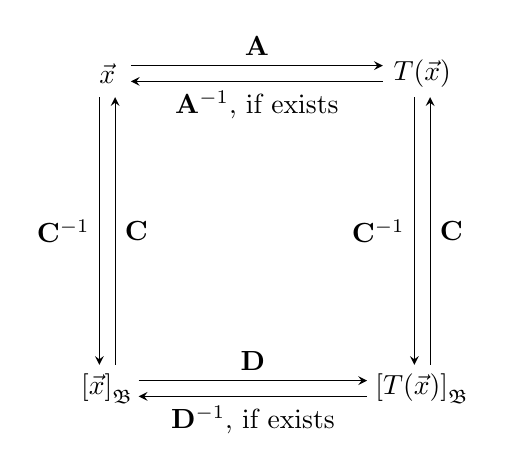
\begin{tikzpicture}
        \node at (-2, 2) {$\vec{x}$};
        \node at (2, 2) {$T(\vec{x})$};
        \node at (-2, -2) {$\coordb{\vec{x}}{\bas{B}}$};
        \node at (2, -2) {$\coordb{T(\vec{x})}{\bas{B}}$};
        \draw[-stealth] (-1.7, 2.1) -- (1.5, 2.1) node[pos=0.5, anchor=south]{$\mat{A}$}; 
        \draw[-stealth] (1.5, 1.9) -- (-1.7, 1.9) node[pos=0.5, anchor=north]{$\invm{A}$, if exists};
        \draw[-stealth] (-2.1, 1.7) -- (-2.1, -1.7) node[pos=0.5, anchor=east]{$\invm{C}$};
        \draw[-stealth] (-1.9, -1.7) -- (-1.9, 1.7) node[pos=0.5, anchor=west]{$\mat{C}$};
        \draw[-stealth] (1.9, 1.7) -- (1.9, -1.7) node[pos=0.5, anchor=east]{$\invm{C}$};
        \draw[-stealth] (2.1, -1.7) -- (2.1, 1.7) node[pos=0.5, anchor=west]{$\mat{C}$};
        \draw[-stealth] (-1.6, -1.9) -- (1.3, -1.9) node[pos=0.5, anchor=south]{$\mat{D}$}; 
        \draw[-stealth] (1.3, -2.1) -- (-1.6, -2.1) node[pos=0.5, anchor=north]{$\invm{D}$, if exists};
    \end{tikzpicture}
    \caption{Transition diagram for linear transformations with respect to bases.}
    \label{fig: linear transformation with respect to bases}
\end{figure}

Figure \ref{fig: linear transformation with respect to bases} tells us that applying matrix $\mat{D}$ on $\coordb{\vec{x}}{\bas{B}}$ to get $\coordb{T(\vec{x})}{\bas{B}}$ is equivalent to applying $\mat{C}$ to get $\vec{x}$, applying $\mat{A}$ to get $T(\vec{x})$, and finally applying $\invm{C}$ to get $\coordb{T(\vec{x})}{\bas{B}}$. From this same diagram, we can also observe that $\mat{A} = \mat{C}\mat{D}\invm{C}$.

This expression of $\mat{D}$ motivates Definition \ref{defn: similar matrices}.
\begin{definition}[similar matrices]
    \label{defn: similar matrices}
    Let $\mat{A}$ and $\mat{B}$ be $n \times n$ matrices. We say $\mat{A}$ is similar to $\mat{B}$ if and only if there exists an invertible matrix $\mat{S}$ such that
    \[\mat{A}\mat{S} = \mat{S}\mat{B},\]
    i.e.
    \[\mat{B} = \invm{S}\mat{A}\mat{S}.\]
    
    The term \textit{similar} is used here because $\mat{A}$ and $\mat{B}$ do essentially the same thing (the same transformation), but in different bases, and hence similar.
\end{definition}
Hence $\mat{A}$ is similar to $\mat{D}$. 

We will now derive an equivalent expression for $\mat{D}$ using linearity of coordinates. Pick any $\vec{x} \in \R^n$. Then, $\vec{x} = c_1\vec{v}_1 + c_2\vec{v}_2 + \cdots + c_n\vec{v}_n$. Hence,
\begin{align*}
    \coordb{T(\vec{x})}{\bas{B}} &= \coordb{T(c_1\vec{v}_1 + c_2\vec{v}_2 + \cdots + c_n\vec{v}_n)}{\bas{B}} \\
    &= \coordb{c_1T(\vec{v}_1) + c_2T(\vec{v}_2) + \cdots + c_nT(\vec{v}_n)}{\bas{B}} & \because \text{Linearity of L.T.} \\
    &= c_1\coordb{T(\vec{v}_1)}{\bas{B}} + c_2\coordb{T(\vec{v}_2)}{\bas{B}} + \cdots + c_n\coordb{T(\vec{v}_n)}{\bas{B}} & \because \text{Linearity of coordinates} \\
    &= \begin{bmatrix}\vert & \vert & & \vert \\ \coordb{T(\vec{v}_1)}{\bas{B}} & \coordb{T(\vec{v}_2)}{\bas{B}} & \cdots & \coordb{T(\vec{v}_n)}{\bas{B}} \\ \vert & \vert && \vert
    \end{bmatrix}\vecxxdx[c] \\
    &= \underbrace{\begin{bmatrix}\vert & \vert & & \vert \\ \coordb{T(\vec{v}_1)}{\bas{B}} & \coordb{T(\vec{v}_2)}{\bas{B}} & \cdots & \coordb{T(\vec{v}_n)}{\bas{B}} \\ \vert & \vert && \vert
    \end{bmatrix}}_{\mat{D}} \coordb{\vec{x}}{\bas{B}} \\
    &= \mat{D}\coordb{\vec{x}}{\bas{B}}.
\end{align*}

These two expressions lead to Theorem \ref{thm: linear transformations with respect to bases}.

\begin{theorem}[Linear transformations with respect to bases]
\label{thm: linear transformations with respect to bases}
    Let $T:\R^n \to \R^n$ be a linear transformation represented by $\mat{A}$, and let $\bas{B} = \left(\vec{v}_1, \vec{v}_2,\cdots,\vec{v}_n\right)$ be a basis for $\R^n$. Then, 
    \[\mat{D} = \begin{bmatrix}\vert & \vert & & \vert \\ \coordb{T(\vec{v}_1)}{\bas{B}} & \coordb{T(\vec{v}_2)}{\bas{B}} & \cdots & \coordb{T(\vec{v}_n)}{\bas{B}} \\ \vert & \vert && \vert
    \end{bmatrix}\]
    is the $\bas{B}$-matrix of $T$.
    
    Let $\mat{C}$ be the change-of-basis matrix with respect to $\bas{B}$. Then, 
    \[\mat{D} = \invm{C}\mat{A}\mat{C}\]
    and
    \[\mat{A} = \mat{C}\mat{D}\invm{C}.\]
\end{theorem}

\begin{example}
    \label{expl: find B-matrix 1}
    Let $T:\R^2 \to \R^2$ be a linear transformation such that $T(\vec{x}) = \underbrace{\begin{bmatrix}3&-2\\2&-2\end{bmatrix}}_{\mat{A}}\vec{x}$. Let $\bas{B} = \left(\colvec{2}{1}{2},\colvec{2}{2}{1}\right)$. Find $\mat{D}$, the transformation matrix of $T$ with respect to $\bas{B}$, then verify that this $\mat{D}$ is correct using an example $\vec{x} = \colvec{2}{1}{-1}$.
\begin{solution}
    The change of basis matrix for $\bas{B}$ is
    \[\mat{C} = \begin{bmatrix}1&2 \\ 2&1\end{bmatrix}\] with \[\invm{C} = -\frac{1}{3}\begin{bmatrix}1&-2\\-2&1\end{bmatrix}.\]
    
    Therefore,
    \[
        \mat{D} = \invm{C} \mat{A}\mat{C} 
        = -\frac{1}{3}\begin{bmatrix}1&-2\\-2&1\end{bmatrix}\begin{bmatrix}3&-2\\2&-2\end{bmatrix}\begin{bmatrix}1&2 \\ 2&1\end{bmatrix} 
        = \begin{bmatrix} -1 & 0 \\ 0 & 2 \end{bmatrix}.
    \]
    
    To verify our $\mat{D}$ is correct, we first compute $T(\vec{x}) = \mat{A}\vec{x} = \colvec{2}{5}{4}$. 
    
    Now, $\coordb{\vec{x}}{\bas{B}} = -\frac{1}{3}\colvec{2}{3}{-3}$. Applying $\mat{D}$ on $\coordb{\vec{x}}{\bas{B}}$ gives us $\coordb{T(\vec{x})}{\bas{B}} = \colvec{2}{1}{2}$. To recompute $T(\vec{x})$ from $\coordb{T(\vec{x})}{\bas{B}}$, we apply $\mat{C}$ on $\coordb{T(\vec{x})}{\bas{B}}$ to get $T(\vec{x}) = \colvec{2}{5}{4}$ which equals what we got before.
    \hfill \qedsymbol
\end{solution}
\end{example}

\begin{example}
    \label{expl: find B-matrix 2}
    Let $\bas{B} = \left(\vec{v}_1,\vec{v}_2,\vec{v}_3\right)$ be any basis of $\R^3$. Find the $\bas{B}$-matrix for linear transformation
    \[T(\vec{x}) = (\vec{v}_2\cdot\vec{x})\vec{v}_2.\]
\begin{solution}
    Using the first part of Theorem \ref{thm: linear transformations with respect to bases}, we have
    \begin{align*}
        \mat{M} &= \begin{bmatrix}\vert & \vert & \vert \\ \coordb{(\vec{v}_2 \cdot \vec{v}_1)\vec{v}_2}{\bas{B}} & \coordb{(\vec{v}_2 \cdot \vec{v}_2)\vec{v}_2}{\bas{B}} &  \coordb{(\vec{v}_2 \cdot \vec{v}_3)\vec{v}_2}{\bas{B}} \\ \vert & \vert & \vert
        \end{bmatrix}.
    \end{align*}
    Since $\coordb{x\vec{v}_2}{\bas{B}} = \colvec{3}{0}{x}{0}$ for $x \in \R$, we have
    \[\mat{M} = \begin{bmatrix}0&0&0 \\ \vec{v}_2 \cdot \vec{v}_1 & \vec{v}_2 \cdot \vec{v}_2 & \vec{v}_2 \cdot \vec{v}_3 \\ 0&0&0\end{bmatrix}.\] \hfill \qedsymbol
\end{solution}
\end{example}

But why? At what cost? Having to compute this daunting product $\invm{C}\mat{A}\mat{C}$ just to perform our transformation in another basis, and eventually having to convert back to Cartesian coordinates. Why?

Take another look at Example \ref{expl: find B-matrix 1}, and observe that applying $\mat{A}$ on an arbitrary vector $\vec{x}$ in our standard basis is more tedious than applying $\mat{D}$ on $\coordb{\vec{x}}{\bas{B}}$, since $\mat{D}$ is a diagonal matrix. Applying it once might not show the difference - but what if we need to compute $\mat{A}^{100} \vec{x}$? The extra efforts for converting $\vec{x}$ to $\coordb{\vec{x}}{\bas{B}}$, computing $\mat{D}^{100}\coordb{\vec{x}}{\bas{B}}$ (much easier due to diagonality), and converting back to our standard basis now seem insignificant. 

This, hopefully, leads naturally to Section \ref{section: the art of choosing bases}.

\subsection{The Art of Choosing Bases}
\label{section: the art of choosing bases}
TODO TODO TODO

\section{Orthogonal Complements}
We start with an example.
\begin{example}
    \label{expl: visualizing image, rowspace, kernel, left kernel}
    Let $\mat{A} = \begin{bmatrix}2&-1&-3\\-4&2&6\end{bmatrix}$. We have
    \[\rref\mat{A} = \begin{bmatrix}[ccc]1 & -1/2 & -3/2 \\ 0&0&0\end{bmatrix},\]
    which tells us that
    \[\kernel\mat{A} = \vecspan\left(\colvec{3}{1/2}{1}{0},\colvec{3}{3/2}{0}{1}\right)\] and that
    \[\image\mat{A} = \vecspan\left(\colvec{2}{2}{-4}\right).\]
    We can now compute the same thing for $\mat{A}^T$. Namely, we can compute $\image\mat{A}^T$, which is equivalent to the rowspace of $\mat{A}$, and $\kernel\mat{A}^T$, which is equivalent to the left kernel of $\mat{A}$. We have
    \[\mat{A}^T = \begin{bmatrix}2 & -4 \\ -1 & 2 \\ -3 & 6\end{bmatrix} \rightsquigarrow \rref\mat{A}^T = \begin{bmatrix}1&-2 \\ 0&0 \\ 0&0\end{bmatrix}.\] Hence,
    \[\kernel\mat{A}^T = \vecspan\left(\colvec{2}{2}{1}\right)\] and \[\image\mat{A}^T = \vecspan\left(\colvec{3}{2}{-1}{3}\right).\]
    Now, we observe that $\image\mat{A}$ and $\kernel\mat{A}^T$ are orthogonal to each other. Indeed,
    \[\colvec{2}{2}{-4} \cdot \colvec{2}{2}{1} = 0.\] Similarly, $\kernel\mat{A}$ and $\image\mat{A}^T$ are orthogonal too:
    \[\colvec{3}{1/2}{1}{0} \cdot \colvec{3}{2}{-1}{3} = \colvec{3}{3/2}{0}{1} \cdot \colvec{3}{2}{-1}{3} = 0.\]
    \hfill \qedsymbol
\end{example}

The conclusion we made in Example \ref{expl: visualizing image, rowspace, kernel, left kernel} is not a coincidence, motivating the definition of \textit{orthogonal complements} in Definition \ref{defn: orthogonal complements}.
\begin{definition}[orthogonal complements]
    \label{defn: orthogonal complements}
    Let $V$ be some subspace in $\R^n$. We define the \textbf{orthogonal complement of $\pmb{V}$} as the linear subspace
    \[V^{\perp} = \left\{\vec{x} \in \R^n \suchthat \vec{x} \cdot \vec{v} = 0 \forall \vec{v} \in V\right\}.\]
    In other words, $V^{\perp}$ contains all vectors perpendicular to all vectors in $V$. We can further declare that if $V_1 = V_2^{\perp}$, then $V_2 = V_1^{\perp}$, which we can prove using Theorem \ref{thm: orthogonal complement of orthogonal complement}.
\end{definition}
The proof for $V^{\perp}$ to be a linear subspace is quite trivial. 

We can now prove the conclusion we made in Example \ref{expl: visualizing image, rowspace, kernel, left kernel} in Theorem \ref{thm: orthogonalities of kernel, left kernel, image, and rowspace}.

\begin{theorem}[Orthogonalities of kernel, left kernel, image, and rowspace]
    \label{thm: orthogonalities of kernel, left kernel, image, and rowspace}
    Let $\mat{A}$ be an $m \times n$ matrix. Then, 
    \[\kernel\mat{A} = \left(\image\mat{A}^T\right)^{\perp}\]
    and
    \[\kernel\mat{A}^T = \left(\image\mat{A}\right)^{\perp}.\]
\begin{proof}
    Let $\mat{A} = \begin{bmatrix} - & \vec{r}_1^T & - \\ - & \vec{r}_2^T & - \\ &\vdots& \\ - & \vec{r}_m^T & -\end{bmatrix}$. 
    
    Pick any $\vec{v} \in \kernel\mat{A}$, and pick any $\vec{w} \in \image\mat{A}^T$. Since $\vec{v} \in \kernel\mat{A}$, it must be the case that $\mat{A}\vec{v} = \vec{0}$. Therefore, for all $\vec{r}_i \cdot \vec{v} = 0$ for all $1 \leq i \leq m$.
    
    Since $\vec{w} \in \image\mat{A}^T$, $w = c_1\vec{r}_1 + c_2\vec{r}_2 + \cdots + c_m\vec{r}_m$ for $c_i \in \R$. Now, we compute
    \[\vec{v} \cdot \vec{w} = \vec{v} \cdot (c_1\vec{r}_1 + c_2\vec{r}_2 + \cdots + c_m\vec{r}_m) = c_1\vec{v}\cdot\vec{r}_1 + \cdots + c_m\vec{v}\cdot\vec{r}_m = 0\] since $\vec{r}_i \cdot \vec{v} = 0$ (shown above for all $1 \leq i \leq m$). 
    
    We have shown that any $\vec{v} \in \kernel\mat{A}$ and $\vec{w} \in \image\mat{A}^T$ must be orthogonal, and hence \[\kernel\mat{A} = \left(\image\mat{A}^T\right)^{\perp}.\]
    
    Now let $\mat{B}^T$ be the transpose of some $\mat{B}$. Then, plugging into the previous equation, we have
    \[\kernel\mat{B}^T = \left(\image\left(\mat{B}^T\right)^T\right)^{\perp} = \left(\image\mat{B}\right)^{\perp}.\]
\end{proof}
\end{theorem}

\subsection{Neat Properties of Orthogonal Complements}

Let $V \subseteq \R^n$ be a linear subspace spanned by vectors $\vec{v}_1,\vec{v}_2,\cdots,\vec{v}_k$. Then, we know that $V$ is the image of matrix $\mat{A} = \begin{bmatrix} \vert & \vert && \vert \\ \vec{v}_1 & \vec{v}_2 & \cdots & \vec{v}_k \\ \vert & \vert && \vert \end{bmatrix}$, i.e. $V = \image\mat{A}$, and hence $\spacedim V = \spacedim\image\mat{A} = k$. We will use the Rank-Nullity Theorem (Theorem \ref{thm: rnt}) to study about $\dim V^{\perp}$. 

By Theorem \ref{thm: orthogonalities of kernel, left kernel, image, and rowspace}, $\kernel\mat{A}^T = \left(\image\mat{A}\right)^{\perp} = V^{\perp}$. Hence, $\dim V^{\perp} = \spacedim\kernel\mat{A}^T$. 

By the Rank-Nullity Theorem, we have
\[\dim\image\mat{A}^T + \dim\kernel\mat{A}^T = n\] because $\mat{A}^T$ is a $k \times n$ matrix. Since $\dim\image\mat{A}^T = \rank\mat{A}^T = \rank\mat{A} = \dim\image\mat{A} = \dim V$, and since $\dim\kernel\mat{A}^T = \dim V^{\perp}$, we have
\[\dim V + \dim V^{\perp} = n.\] Once again, recall that $V \subseteq \R^n$. 

We summarize this finding in Theorem \ref{thm: dimensions of subspaces and their orthogonal complement}.
\begin{theorem}[Dimensions of subspaces and their orthogonal complements]
    \label{thm: dimensions of subspaces and their orthogonal complement}
    Let $V \subseteq \R^n$ be a linear subspace. Then,
    \[\dim V + \dim V^{\perp} = n.\]
\end{theorem}

We can visualize this result, using our familiar diagram in Figure \ref{fig: V and V-perp}, which illustrates a plane $V$ and its orthogonal complement $V^{\perp}$ (which is a line orthogonal to $V$) in $\R^3$. As clearly seen,
\[\dim V + \dim V^{\perp} = 2 + 1 = 3 = n.\]

\begin{figure}
    \centering
    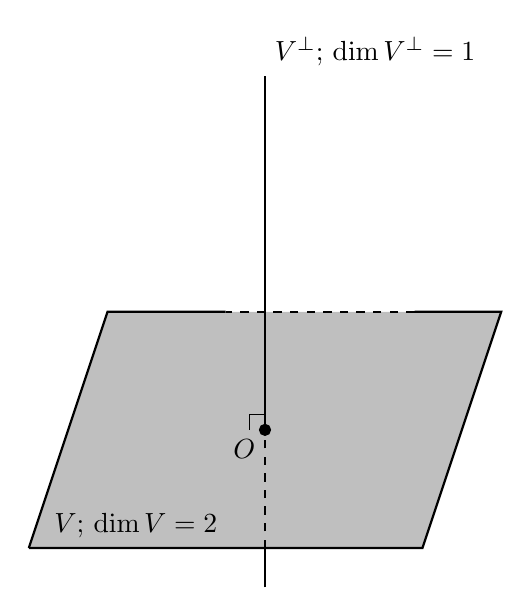
\begin{tikzpicture}
        \draw[fill=lightgray, draw=none] (0,0) -- (5,0) -- (6,3) -- (1, 3) -- cycle;
        \draw[thick] (0,0) -- (5,0) -- (6,3) -- (4.9, 3); % -- (1,4) -- cycle;
        \draw[thick,dashed] (4.9, 3) -- (2.5,3);
        \draw[thick] (2.5, 3) -- (1,3) -- (0,0);
        \node[anchor = south west] at (0.2, 0) {$V$; $\dim V = 2$}; 
        \filldraw (3,1.5) circle (2pt) node[anchor=north east]{$O$};
        \draw (3,1.5) -- (3,6) node[anchor=south west]{$V^{\perp}$; $\dim V^{\perp} = 1$};
        \draw[dashed] (3,0) -- (3,1.5);
        \draw (3,-0.5) -- (3,0);
        \draw (3, 1.7) -- (2.8, 1.7) -- (2.8, 1.5);
    \end{tikzpicture}
    \caption{Subspaces $V$ and $V^{\perp}$}
    \label{fig: V and V-perp}
\end{figure}

Now, the following thing may confuse a bit: the Rank-Nullity Theorem says that $\dim\image\mat{A} + \dim\kernel\mat{A} = n$, and in our case, $\dim\image\mat{A} = \dim V$. However, this only tells us that $\dim\kernel\mat{A} = \dim V^{\perp}$, but it tells us nothing about whether $\kernel\mat{A} = V^{\perp}$, or whether $\kernel\mat{A} = \left(\image\mat{A}\right)^{\perp}$, despite them having the same dimension. Matrices $\mat{A}$ and $\mat{A}^T$ share the same \textit{nullity}, but may indeed be different subspaces. Our figure just happens to show an example where these are equal.


\begin{theorem}[Intersection of a subspace and its orthogonal complement]
    \label{thm: intersection of a subspace and its orthogonal complement}
    Let $V \subseteq \R^n$ be a linear subspace. Then, $V \cap V^{\perp} = \left\{\vec{0}\right\}$. 
\begin{proof}
    Suppose $\vec{x} \in V \cap V^{\perp}$. Then, since $\vec{x} \in V^{\perp}$, by definition, for all $\vec{v} \in V$, \[\vec{x} \cdot \vec{v} = 0.\]
    In particular, $\vec{x} \in V$, 
    \[\vec{x} \cdot \vec{x} = 0,\]
    which means $\left\|\vec{x}\right\|^2 = 0$, i.e. $\vec{x} = \vec{0}$. 
\end{proof}
\end{theorem}

We will now show that any $\vec{x} \in \R^n$ can be written as $\vec{v} + \vec{w}$ for some unique $\vec{v} \in V$ and $\vec{w} \in V^{\perp}$, in Theorem \ref{thm: representing R^n using V and V^perp}.

\begin{theorem}[Representing $\R^n$ using $V$ and $V^{\perp}$]
    \label{thm: representing R^n using V and V^perp}
    Let $V \subseteq \R^n$ be a linear subspace. Then, any $\vec{x} \in \R^n$ can be written as $\vec{v} + \vec{w}$ for some unique $\vec{v} \in V$ and $\vec{w} \in V^{\perp}$. 
\begin{proof}
    We first prove existence of such $\vec{v}$ and $\vec{w}$. Suppose $\dim{V} = k$ for some $k \leq n$. Then, by Theorem \ref{thm: dimensions of subspaces and their orthogonal complement}, we have $\dim{V^{\perp}} = n-k$. Then, any basis of $V$ has $k$ vectors, and any basis of $V^{\perp}$ has $n-k$ vectors. 
    
    Suppose $\bas{B}_V = \left\{\vec{v}_1,\vec{v}_2,\cdots,\vec{v}_k\right\}$ forms a basis for $V$ and $\bas{B}_{V^{\perp}} = \left\{\vec{w}_1,\vec{w}_2,\cdots,\vec{w}_{n-k}\right\}$ forms a basis for $V^{\perp}$. We will show that \[\bas{B}_V \cup \bas{B}_{V^{\perp}} = \left\{\vec{v}_1,\vec{v}_2,\cdots,\vec{v}_k, \vec{w}_1,\vec{w}_2,\cdots,\vec{w}_{n-k}\right\}\] is a linearly independent set of vectors, and hence $\bas{B}_V \cup \bas{B}_{V^{\perp}}$ forms a basis for $\R^n$. 
    
    We examine the solution set for equation 
    \[c_1\vec{v}_1 + c_2\vec{v}_2 + \cdots + c_k\vec{v}_k + d_1\vec{w}_1 + d_2\vec{w}_2 + \cdots + d_{n-k}\vec{w}_{n-k} = \vec{0},\]
    which we rearrange to get
    \[c_1\vec{v}_1 + c_2\vec{v}_2 + \cdots + c_k\vec{v}_k = -\left(d_1\vec{w}_1 + d_2\vec{w}_2 + \cdots + d_{n-k}\vec{w}_{n-k}\right).\]
    
    Now let $\vec{x} = c_1\vec{v}_1 + c_2\vec{v}_2 + \cdots + c_k\vec{v}_k$. Then,
    \[\vec{x} = \underbrace{c_1\vec{v}_1 + c_2\vec{v}_2 + \cdots + c_k\vec{v}_k}_{\vec{x} \in V} = \underbrace{-\left(d_1\vec{w}_1 + d_2\vec{w}_2 + \cdots + d_{n-k}\vec{w}_{n-k}\right)}_{\vec{x} \in V^{\perp}}.\]
    
    Since $\vec{x} \in V$ and $\vec{x} \in V^{\perp}$, by Theorem \ref{thm: intersection of a subspace and its orthogonal complement}, $\vec{x} = \vec{0}$. Hence, 
    \[c_1\vec{v}_1 + c_2\vec{v}_2 + \cdots + c_k\vec{v}_k = \vec{0}.\] Since $\vec{v}_1,\vec{v}_2,\cdots,\vec{v}_k$ are linearly independent, then, $c_1 = c_2 = \cdots = c_k = 0$. Similarly, we can conclude that $d_1 = d_2 = \cdots = d_{n-k} = 0$. Hence, $\bas{B}_{V} \cup \bas{B}_{V^{\perp}}$ is a linearly independent set of vectors, and hence $\bas{B}_{V} \cup \bas{B}_{V^{\perp}}$ forms a basis for $\R^n$. 
    
    Therefore, pick any $\vec{x} \in \R^n$. Then, 
    \[\vec{x} = \underbrace{c_1\vec{v}_1 + c_2\vec{v}_2 + \cdots + c_k\vec{v}_k}_{\vec{v} \in V} + \underbrace{d_1\vec{w}_1 + d_2\vec{w}_2 + \cdots + d_{n-k}\vec{w}_{n-k}}_{\vec{w} \in V^{\perp}},\]
    i.e.
    \[\vec{x} = \vec{v} + \vec{w}\] for $\vec{v} \in V$ and $\vec{w} \in V^{\perp}$. 
    
    Now we will prove uniqueness of this representation. Suppose $\vec{x} \in \R^n$, and suppose
    \[\vec{x} = \vec{v}_1 + \vec{w}_1 = \vec{v}_2 + \vec{w}_2\] for $\vec{v}_1,\vec{v}_2 \in V$ and $\vec{w}_1,\vec{w}_2 \in V^{\perp}$.
    We can rearrange this equation and let $\vec{z} = \vec{v}_1 - \vec{v}_2$ to yield
    \[\vec{z} = \underbrace{\vec{v}_1 - \vec{v}_2}_{\vec{z} \in V} = \underbrace{\vec{w}_1 - \vec{w}_2}_{\vec{z} \in V^{\perp}}.\]
    By Theorem \ref{thm: intersection of a subspace and its orthogonal complement}, then, $\vec{z} = \vec{0}$, so $\vec{v}_1 - \vec{v}_2 = \vec{w}_1 - \vec{w}_2 = 0$, which tells us that $\vec{v}_1 = \vec{v}_2$ and $\vec{w}_1 = \vec{w}_2$. Hence, this representation is unique.
\end{proof}
\end{theorem}

Now we can prove that $\left(V^{\perp}\right)^{\perp} = V$ in Theorem \ref{thm: orthogonal complement of orthogonal complement}.
\begin{theorem}[Orthogonal complement of orthogonal complement]
    \label{thm: orthogonal complement of orthogonal complement}
    Let $V \subseteq \R^n$ be a linear subspace. Then, $\left(V^{\perp}\right)^{\perp} = V$.
\begin{proof}
    It's trivial to see that $\left(V^{\perp}\right)^{\perp} \subseteq \R^n$.
    
    Suppose $\vec{x} \in \left(V^{\perp}\right)^{\perp}$. Then, since $\left(V^{\perp}\right)^{\perp} \subseteq \R^n$, by Theorem \ref{thm: representing R^n using V and V^perp}, we have
    \[\vec{x} = \vec{v} + \vec{w}\] for some $\vec{v} \in V$ and $\vec{w} \in V^{\perp}$. Let's take the dot product of both sides by $\vec{w}$:
    \[\vec{x} \cdot \vec{w} = (\vec{v} + \vec{w}) \cdot \vec{w} = \vec{v}\cdot\vec{w} + \vec{w}\cdot\vec{w}.\]
    
    Since $\vec{x} \in \left(V^{\perp}\right)^{\perp}$ and $\vec{w} \in V^{\perp}$, $\vec{x} \cdot \vec{w} = 0$ by definition. Since $\vec{v} \in V$ and $\vec{w} \in V^{\perp}$, $\vec{v} \cdot \vec{w} = 0$. Hence,
    \[\vec{w} \cdot \vec{w} = 0\] and hence $\vec{w} = \vec{0}$.
    Therefore,
    \[\vec{x} = \vec{v} + \vec{0} = \vec{v} \in V,\] i.e. $\left(V^{\perp}\right)^{\perp} \subseteq V$.
    
    Similarly, suppose $\vec{x} \in V$. Then, since $V \subseteq \R^n$, by Theorem \ref{thm: representing R^n using V and V^perp}, we have
    \[\vec{x} = \vec{v} + \vec{w}\] for $\vec{v} \in V^{\perp}$ and $\vec{w} \in \left(V^{\perp}\right)^{\perp}$. We take the dot product of both sides with $\vec{v}$ to get
    \[\vec{x} \cdot \vec{v} = \vec{v} \cdot \vec{v} + \vec{w} \cdot \vec{v}.\] Since $\vec{x} \cdot \vec{v} = 0$ and $\vec{w} \cdot \vec{v} = 0$, we have
    \[\vec{v} \cdot \vec{v} = 0\] which tells us that $\vec{v} = \vec{0}$. Hence,
    \[\vec{x} = \vec{0} + \vec{w} = \vec{w} \in \left(V^{\perp}\right)^{\perp},\] i.e. $V \subseteq \left(V^{\perp}\right)^{\perp}$. 
    
    Therefore,
    \[\left(V^{\perp}\right)^{\perp} = V.\]
\end{proof}
\end{theorem}

Using these neat properties, we will prove a technical result that will be useful later.

\begin{theorem}[Kernel and invertibility of $\mat{A}^T\mat{A}$]
    \label{thm: kernel and invertibility of A^T x A}
    Let $\mat{A}$ be an $n \times m$ matrix. Then, \begin{enumerate}
        \item $\kernel\mat{A} = \kernel\mat{A}^T\mat{A}$, and
        \item if $\kernel\mat{A} = \left\{\vec{0}\right\}$, then $\mat{A}^T\mat{A}$ is invertible.
    \end{enumerate}
\begin{proof}
    We begin with the first claim. We will show that the two sets are subsets of each other.
    
    Pick any $\vec{x} \in \kernel\mat{A}$. Then, $\mat{A}\vec{x} = \vec{0}$. Since $\mat{A}^T\vec{0} = \vec{0}$, we have $\mat{A}^T\mat{A}\vec{x} = \vec{0}$. It then naturally follows that $\vec{x} \in \kernel\mat{A}^T\mat{A}$.
    
    Now, pick any $\vec{y} \in \kernel\mat{A}^T\mat{A}$. Then, it follows that $\mat{A}^T\mat{A}\vec{y} = \vec{0}$. From this, we know that $\mat{A}\vec{y} \in \kernel\mat{A}^T$. Since it is trivial that $\mat{A}\vec{y} \in \image\mat{A}$, and since $\image\mat{A}$ is the orthogonal complement of $\kernel\mat{A}^T$ (see Theorem \ref{thm: orthogonalities of kernel, left kernel, image, and rowspace}), by Theorem \ref{thm: intersection of a subspace and its orthogonal complement}, $\mat{A}\vec{y} = \vec{0}$. Therefore, $\vec{y} \in \kernel\mat{A}$.
    
    Hence, $\kernel\mat{A} = \kernel\mat{A}^T\mat{A}$, hence proving the first claim.
    
    Now, suppose $\kernel\mat{A} = \left\{\vec{0}\right\}$. Then, by our first claim, $\kernel\mat{A}^T\mat{A} = \kernel\mat{A} = \left\{\vec{0}\right\}$, and hence $\mat{A}^T\mat{A}$ has linearly independent columns (see Theorem \ref{thm:null space linear dependence}). 
    
    Therefore, by Theorem \ref{thm: A-transpose x A is invertible}, $\mat{A}^T\mat{A}$ is invertible. 
\end{proof}
\end{theorem}
\subsection{Unique Rowspace Solutions to Matrix Equations}
Let $\mat{A}$ be an $m \times n$ matrix, and suppose $\vec{b} \in \image\mat{A}$. Then, by Theorem \ref{thm:column space}, we have that $\mat{A}\vec{x} = \vec{b}$ has at least one solution $\vec{x} \in \R^n$. In this section, we will study a special type of solutions. 

Suppose $\vec{x}$ is a solution to $\mat{A}\vec{x} = \vec{b}$. Since $\vec{x} \in \R^n$, we know that $\vec{x} = \vec{r}_0 + \vec{n}_0$ for some $\vec{r}_0 \in \image\mat{A}^T$ and $\vec{n}_0 \in \kernel\mat{A}$ (see Theorems \ref{thm: orthogonalities of kernel, left kernel, image, and rowspace} and \ref{thm: representing R^n using V and V^perp}). We will now show that $\vec{r}_0$ is also a solution to $\mat{A}\vec{x} = \vec{b}$ (since $\vec{r}_0$ is in the rowspace of $\mat{A}$, we claim that $\vec{r}_0$ is a rowspace solution to $\mat{A}\vec{x} = \vec{b}$).

We rearrange to have $\vec{r}_0 = \vec{x} - \vec{n}_0$. Then, we have
\[\mat{A}\vec{r}_0 = \mat{A}(\vec{x} - \vec{n}_0) = \mat{A}\vec{x} - \mat{A}\vec{n}_0.\]
Since $\vec{n}_0 \in \kernel\mat{A}$, $\mat{A}\vec{n}_0 = \vec{0}$, and since $\mat{A}\vec{x} = \vec{b}$, we have
\[\mat{A}\vec{r}_0 = \vec{b},\]
and hence $\vec{r}_0$ is a solution to $\mat{A}\vec{x} = \vec{b}$.

Now, a natural question to ask is whether this $\vec{r}_0$ is unique. Suppose $\vec{r}_1 \in \image\mat{A}^T$ is also a solution to $\mat{A}\vec{x} = \vec{b}$. Since $\image\mat{A}^T$ is a linear subspace, we know that $\vec{r}_1 - \vec{r}_0 \in \image\mat{A}^T$. Now we compute
\[\mat{A}\left(\vec{r}_1 - \vec{r}_0\right) = \mat{A}\vec{r}_1 - \mat{A}\vec{r}_0 = \vec{b} - \vec{b} = \vec{0}.\]
Therefore, $\vec{r}_1 - \vec{r}_0 \in \kernel\mat{A}$. 

Since $\kernel\mat{A}$ and $\image\mat{A}^T$ are orthogonal complements, and since $\vec{r}_1 - \vec{r}_0 \in \kernel\mat{A}$ and $\vec{r}_1 - \vec{r}_0 \in \image\mat{A}^T$, by Theorem \ref{thm: intersection of a subspace and its orthogonal complement}, we conclude that $\vec{r}_1 - \vec{r}_0 = \vec{0}$, and hence $\vec{r}_1 = \vec{r}_0$, proving that these rowspace solutions are unique.

We will now study an interesting and neat property of these rowspace solutions.

Recall the original definition of $\vec{x}$ in this section. We now take
\[\left\|\vec{x}\right\|^2 = \vec{x} \cdot \vec{x} = \left(\vec{r}_0 + \vec{n}_0\right) \cdot \left(\vec{r}_0 + \vec{n}_0\right) = \vec{r}_0 \cdot \vec{r}_0 + 2\vec{r}_0\cdot\vec{n}_0 + \vec{n}_0 \cdot \vec{n}_0.\]
Since $\vec{r}_0$ and $\vec{n}_0$ are orthogonal (because their respective subspaces are orthogonal complements of each other), $\vec{r}_0 \cdot \vec{n}_0 = 0$, leaving us
\[\left\|\vec{x}\right\|^2 = \vec{r}_0 \cdot \vec{r}_0 + \vec{n}_0 \cdot \vec{n}_0 = \left\|\vec{r}_0\right\|^2 + \left\|\vec{n}_0\right\|^2.\]

Since $\left\|\vec{n}_0\right\|^2 \geq 0$, we have
\[\left\|\vec{x}\right\|^2 \geq \left\|\vec{r}_0\right\|^2,\]
i.e.
\[\left\|\vec{r}_0\right\| \leq \left\|\vec{x}\right\|.\]

This result tells us that the unique rowspace solution to $\mat{A}\vec{x} = \vec{b}$ always has minimal possible length.

We conclude this finding in Theorem \ref{thm: unique minimum rowspace solution}.

\begin{theorem}[Unique minimum rowspace solution]
    \label{thm: unique minimum rowspace solution}
    Let $\mat{A}$ be a matrix, and suppose $\vec{b} \in \image\mat{A}$. Then, there exists a unique $\vec{r}_0 \in \image\mat{A}^T$ such that $\mat{A}\vec{r}_0 = \vec{b}$, and no other solution $\vec{x}$ can have a smaller length than $\vec{r}_0$.
\end{theorem}

\begin{example}
    \label{expl: shortest rowspace solution}
    Let $\mat{A} = \begin{bmatrix}3 & -2 \\ 6 & -4\end{bmatrix}$, and let $\vec{b} = \colvec{2}{9}{18}$. It is not difficult to compute that the solution set to $\mat{A}\vec{x} = \vec{b}$ is $S = \left\{\colvec{2}{3}{0} + c\colvec{2}{2}{3} \suchthat c \in \R\right\}$. Find the solution with the shortest length.
\begin{solution}
    By Theorem \ref{thm: unique minimum rowspace solution}, the solution of the shortest length is some $\vec{r}_0 \in \image\mat{A}^T$. We have $\mat{A}^T = \begin{bmatrix}3 & 6 \\ -2 & -4 \end{bmatrix}$. Since the second column is twice the first column, it's redundant, so $\image\mat{A}^T = \vecspan\colvec{2}{3}{-2}$, i.e. $\vec{r}_0 = t\colvec{2}{3}{-2}$. 
    
    Since $\vec{r}_0$ is, after all, a solution, we have $\vec{r}_0 = \colvec{2}{3}{0} + c\colvec{2}{2}{3}$. 
    Let $\vec{r}_0 = \colvec{2}{a}{b}$. Then, we set up equation
    \begin{align*}
        \colvec{2}{a}{b} &= \colvec{2}{3}{0} + c\colvec{2}{2}{3} \\
        \colvec{2}{a}{b} &= t\colvec{2}{3}{-2}.
    \end{align*}
    We have
    \[\colvec{2}{3}{0} + c\colvec{2}{2}{3} = t\colvec{2}{3}{-2},\] we solve that
    \[t = \frac{9}{13},\]
    which means $\vec{r}_0 = \frac{9}{13}\colvec{2}{3}{-2}$.
    
    For the sake of a more complete example, we will graph $\kernel\mat{A}$, the solution set $S$ listed above, and $\image\mat{A}^T$ in Figure \ref{fig: expl: shortest rowspace solution}. Indeed, $S$ is nothing but $\kernel\mat{A}$ shifted by $\colvec{2}{3}{0}$ (see Theorem \ref{thm: solution set and null space}).
    
    Observe, in the diagram, that $\vec{x} - \vec{r}_0 = \vec{x} - t\colvec{2}{3}{-2}$ is orthogonal to $\colvec{2}{3}{-2}$ which spans $\image\mat{A}^T$, for an arbitrary solution $\vec{x}$. We can use solution $\vec{x} = \colvec{2}{3}{0}$ and this fact to solve for $t$:
    \[\left(\colvec{2}{3}{0} - t\colvec{2}{3}{-2}\right)\cdot\colvec{2}{3}{-2} = 0.\]
    We can solve that $t = \frac{9}{13}$. \hfill \qedsymbol
    
\end{solution}
\end{example}

\begin{figure}
    \centering
    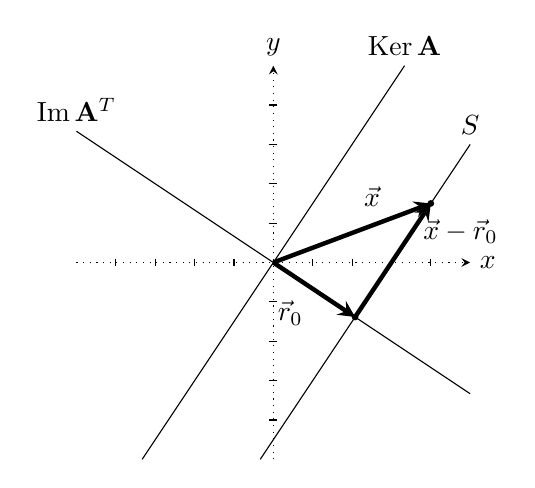
\begin{tikzpicture}[scale=0.5]
        \draw[dotted, -stealth] (-5, 0) -- (5, 0) node[anchor=west]{$x$};
        \draw[dotted, -stealth] (0, -5) -- (0, 5) node[anchor=south]{$y$};
        \foreach \xval in {-4,-3,-2,-1, 1, 2, 3, 4}
            \draw (\xval, 0.1) -- (\xval, -0.1);
        \foreach \yval in {-1, -2, -3, -4, 1, 2, 3, 4}
            \draw (0.1, \yval) -- (-0.1, \yval);
        
        \draw (-10/3,-5) -- (10/3, 5) node[anchor=south]{$\kernel\mat{A}$};
        \draw (-1/3, -5) -- (5, 3) node[anchor=south]{$S$};
        \draw (5, -10/3) -- (-5, 10/3) node[anchor=south]{$\image\mat{A}^T$};
        \filldraw (27/13, -18/13) circle (2pt);
        \draw[ultra thick, -stealth] (0,0) -- (27/13, -18/13) node[pos=0.5, anchor=north east]{$\vec{r}_0$};
        \draw[ultra thick, -stealth](0,0) -- (4, 1.5) node[pos=0.75, anchor=south east]{$\vec{x}$};
        \filldraw (4,1.5) circle (2pt);
        \draw[ultra thick, -stealth](27/13, -18/13) -- (4, 1.5) node[pos=0.75, anchor=west]{$\vec{x} - \vec{r}_0$};
    \end{tikzpicture}
    \caption{Diagram for Example \ref{expl: shortest rowspace solution}}
    \label{fig: expl: shortest rowspace solution}
\end{figure}
    
\section{Orthogonal Projections onto Subspaces}
Recall in Section \ref{section: orthogonal projection transformation}, we introduced a linear transformation $\proj_L$ that transforms a vector $\vec{x} \in \R^n$ to its component on line $L$ passing through the origin, as well as $\proj_V$ that projects $\vec{x}$ onto a plane in $\R^3$ passing through the origin. A line and a plane are linear subspaces (adding two vectors on a line still results in another vector on the same line; scaling a vector on the line still results in another vector on the line; same for planes). In this section, we will study orthogonal projections onto arbitrary linear subspaces.

\begin{definition}[orthogonal projection onto a subspace]
    \label{defn: orthogonal projection onto a subspace}
    Let $V \subseteq \R^n$ be a subspace, and pick any $\vec{x} \in \R^n$. Then, by Theorem \ref{thm: representing R^n using V and V^perp}, $\vec{x} = \vec{v} + \vec{w}$ for $\vec{v} \in V$ and $\vec{w} \in V^{\perp}$.
    
    We define the projection of $\vec{x}$ onto $V$ as
    $\proj_V \vec{x} = \vec{v}$. Similarly, we define the projection of $\vec{x}$ onto $V^{\perp}$ as $\proj_{V^{\perp}}\vec{x} = \vec{w}$.
    
    Naturally, we have $\vec{x} = \proj_V \vec{x} + \proj_{V^{\perp}}\vec{x}$.
\end{definition}

Let $L$ be a line passing through the origin in $\R^n$. In Section \ref{section: orthogonal projection transformation} (in particular, Definition \ref{defn: orthogonal projection}), we derived an expression for the orthogonal projection of $\vec{x}$ onto $L$: $\proj_L \vec{x} = \frac{\vec{x} \cdot \vec{v}}{\vec{v} \cdot \vec{v}} \vec{v}$. We will give an intuition that our new definition is equivalent to this old definition for a line. 

Take another look at Figure \ref{fig: orthogonal projection onto a line}, and observe that $\vec{x} - \proj_L \vec{x}$ is orthogonal to $L$. Let's name $\vec{v} = \proj_L \vec{x}$. Then, $\vec{x} - \vec{v}$ is orthogonal to everything in $L$. Let $\vec{w} = \vec{x} - \vec{v}$, and we rearrange to give
\[\vec{x} = \vec{v} + \vec{w}.\]

Now, $\vec{v} \in L$, and $\vec{w} \in L^{\perp}$ (because $\vec{w}$ is orthogonal to everything in $L$). Indeed, this new definition, once applied to lines, is equivalent to the old definition.

We can now use this new definition, in combination of the previous expression, to tackle a previous example.
\begin{example}
    \label{expl: rowspace solution using orthogonal projection}
    Recall Example \ref{expl: shortest rowspace solution} and its accompanying Figure \ref{fig: expl: shortest rowspace solution}. Observe that for a given $\vec{v} \in \R^2$, it can be written as $\vec{v} = \vec{r} + \vec{n}$ for some $\vec{r} \in \image\mat{A}^T$ and $\vec{n} \in \kernel\mat{A}$ (see Theorem \ref{thm: representing R^n using V and V^perp}).
    
    In particular, let $\vec{x} \in S$ (recall that $S$ is the solution set to the given equation). Then, $\vec{x} = \vec{r}_0 + \vec{n}_0$ for $\vec{r}_0 \in \image\mat{A}^T$ and $\vec{n}_0 \in \kernel\mat{A}$. By Definition \ref{defn: orthogonal projection onto a subspace}, then, $\proj_{\image\mat{A}^T} \vec{x} = \vec{r}_0$. Let $\vec{x} = \colvec{2}{3}{0}$.
    
    From Definition \ref{defn: orthogonal projection}, we compute that \[\proj_{\image\mat{A}^T}\vec{x} = \frac{\colvec{2}{3}{0} \cdot \colvec{2}{3}{-2}}{\colvec{2}{3}{-2} \cdot \colvec{2}{3}{-2}} \colvec{2}{3}{-2} = \frac{9}{13}\colvec{2}{3}{-2}.\]
    
    This is the same as we computed in Example \ref{expl: shortest rowspace solution}. The shortest solution is nothing but the projection of another solution onto the rowspace of the matrix. \hfill \qedsymbol
\end{example}

\subsection{Orthogonal Projections as Linear Transformations}
Let $V$ be a subspace of $\R^n$, and suppose $\bas{B} = (\vec{b}_1,\vec{b}_2,\cdots,\vec{b}_k)$ forms a basis for $V$. Let $\mat{A} = \begin{bmatrix}\vert & \vert && \vert \\ \vec{b}_1 & \vec{b}_2 & \cdots & \vec{b}_k \\ \vert & \vert & & \vert\end{bmatrix}$. Then, for any $\vec{a} \in V$, $\mat{A}\vec{y} = \vec{a}$ for some $\vec{y} \in \R^k$ (this follows directly from the definition of $\bas{B}$ being a basis).

Pick any $\vec{x} \in \R^n$. Then, by definition, $\proj_V \vec{x} \in V$. Therefore, as said above, $\proj_V \vec{x} = \mat{A}\vec{y}$ for some $\vec{y} \in \R^k$. We will find an expression for $\vec{y}$, and show that an orthogonal projection onto a linear subspace is a linear transformation.

Since $\vec{x} \in \R^n$, we can write $\vec{x} = \proj_V \vec{x} + \proj_{V^{\perp}} \vec{x}$, where $ \proj_{V^{\perp}} \vec{x} \in V^{\perp}$. We can rearrange this equation to yield $\vec{x} - \proj_V \vec{x} = \proj_{V^{\perp}}\vec{x}$, and hence $\vec{x} - \proj_V \vec{x} \in V^{\perp}$. Since $V = \image\mat{A}$, $V^{\perp} = \left(\image\mat{A}\right)^T = \kernel\mat{A}^T$ (see Theorem \ref{thm: orthogonalities of kernel, left kernel, image, and rowspace}). Hence, \[\vec{x} - \proj_V \vec{x} \in \kernel\mat{A}^T.\]

By definition of kernels, then,
\[\mat{A}^T\left(\vec{x} - \proj_V \vec{x}\right) = \vec{0} \Longleftrightarrow \mat{A}^T\vec{x} - \mat{A}^T\proj_V \vec{x} = \vec{0} \Longleftrightarrow \mat{A}^T\vec{x} = \mat{A}^T\proj_V\vec{x}.\]

Now recall that $\proj_V \vec{x} = \mat{A}\vec{y}$ for some $\vec{y} \in \R^k$. We substitute this into the previous equation to have
\[\mat{A}^T\vec{x} = \mat{A}^T\mat{A}\vec{y}.\]

By Theorem \ref{thm: A-transpose x A is invertible}, since $\mat{A}$ has linearly independent columns, $\mat{A}^T\mat{A}$ is invertible. We apply $\left(\mat{A}^T\mat{A}\right)^{-1}$ onto both sides to yield
\[\left(\mat{A}^T\mat{A}\right)^{-1}\mat{A}^T\vec{x} = \vec{y}.\]

We now have an expression for $\vec{y}$, so we can rewrite $\proj_V \vec{x}$ as
\[\proj_V \vec{x} = \mat{A}\vec{y} = \underbrace{\mat{A}\left(\mat{A}^T\mat{A}\right)^{-1}\mat{A}^T}_{\text{some matrix}}\vec{x}.\]

Since $\proj_V\vec{x}$ can be written as some matrix-vector product, $\proj_V$ is linear. We summarize this finding in Theorem \ref{thm: matrix of orthogonal projection onto subspace}.

\begin{theorem}[Matrix of orthogonal projection onto subspace]
    \label{thm: matrix of orthogonal projection onto subspace}
    Let $V$ be a linear subspace defined by basis $\bas{B} = \left(\vec{b}_1,\vec{b}_2,\cdots,\vec{b}_k\right)$. Then, 
    $\proj_V \vec{x} = \mat{A}\left(\mat{A}^T\mat{A}\right)^{-1}\mat{A}^T\vec{x}$ for matrix $\mat{A}$ having columns $\vec{b}_1,\vec{b}_2,\cdots,\vec{b}_k$. Hence, $\proj_V$ is a linear transformation.
\end{theorem}

We will now show a couple of examples regarding finding the matrices of orthogonal projections onto subspaces.

\begin{example}
    \label{expl: subspace projection matrix}
    Let $V = \vecspan\left(\colvec{4}{1}{0}{0}{1}, \colvec{4}{0}{1}{0}{1}\right)$ be a linear subspace. It is trivial to see that the two vectors are linearly independent, so they form a basis for $V$. Find a matrix $\mat{M}$ such that $\proj_V\vec{x} = \mat{M}\vec{x}$ for all $\vec{x} \in \R^4$.
\begin{solution}
    Let $\mat{A} = \begin{bmatrix}1&0 \\ 0&1 \\ 0&0 \\ 1&1\end{bmatrix}$. Then, by Theorem \ref{thm: matrix of orthogonal projection onto subspace}, $\mat{M} = \mat{A}\left(\mat{A}^T\mat{A}\right)^{-1}\mat{A}^T$. 
    
    With $\mat{A}^T = \begin{bmatrix}1&0&0&1 \\ 0&1&0&1\end{bmatrix}$, we have
    \[\mat{A}^T\mat{A} = \begin{bmatrix}2&1 \\ 1&2\end{bmatrix}.\]
    Using Theorem \ref{thm: formula for 2x2 inverse}, we have $\left(\mat{A}^T\mat{A}\right)^{-1} = \frac{1}{3}\begin{bmatrix}2&-1\\-1&2\end{bmatrix}$. Therefore,
    \begin{align*}
        \mat{M} &= \mat{A}\left(\mat{A}^T\mat{A}\right)^{-1}\mat{A}^T \\
        &= \begin{bmatrix}1&0 \\ 0&1 \\ 0&0 \\ 1&1\end{bmatrix} \frac{1}{3}\begin{bmatrix}2&-1\\-1&2\end{bmatrix} \begin{bmatrix}1&0&0&1 \\ 0&1&0&1\end{bmatrix} \\
        &= \frac{1}{3}\begin{bmatrix}2&-1&0&1 \\ -1&2&0&1 \\ 0&0&0&0 \\ 1&1&0&2\end{bmatrix}
    \end{align*}
    is the matrix for $\proj_V$. \hfill \qedsymbol
\end{solution}
\end{example}

\begin{example}
    \label{expl: orthogonal projection onto a line, verification}
    Let $\vec{u} = \vecxx[u]$ be a unit vector, and let $L$ be a line spanned by $\vec{u}$. We will use Theorem \ref{thm: matrix of orthogonal projection onto subspace} to derive a matrix for $\proj_L$ and compare our answer with Theorem \ref{thm: 2d projection matrix}.
    
    Let $\mat{A} = \colvec{2}{u_1}{u_2}$ (representing a vector as a matrix here), and hence $\mat{A}^T = \begin{bmatrix}u_1 & u_2\end{bmatrix}$. We now compute
    \[\mat{A}^T\mat{A} = \begin{bmatrix}u_1 & u_2 \end{bmatrix}\colvec{2}{u_1}{u_2} = \begin{bmatrix} u_1^2 + u_2^2 \end{bmatrix} = \begin{bmatrix}1\end{bmatrix}\]
    because $\vec{u}$ is a unit vector.
    
    Hence, the matrix for $\proj_L$ is
    \[
        \mat{A}\left(\mat{A}^T\mat{A}\right)\mat{A}^T = \colvec{2}{u_1}{u_2} \begin{bmatrix}1\end{bmatrix}\begin{bmatrix}u_1 & u_2\end{bmatrix} 
        = \begin{bmatrix}u_1^2 & u_1u_2 \\ u_1u_2 & u_2^2\end{bmatrix}.
    \]
    This is the same as in Theorem \ref{thm: 2d projection matrix}. \hfill \qedsymbol
\end{example}

To end this section, we will show something that will be useful for least-squares (Section \ref{section: introduction to least-squares approximation}) in Theorem \ref{thm: orthogonal projection is the closest vector in subspace}. 

\begin{theorem}[Orthogonal projection is the closest vector in subspace]
    \label{thm: orthogonal projection is the closest vector in subspace}
    Let $V \subseteq \R^n$ be a linear subspace, and suppose $\vec{x} \in V$. Then, 
    \[\left\|\vec{x} - \proj_V \vec{x}\right\| \leq \left\|\vec{x} - \vec{v}\right\|\] for all $\vec{v} \in V$. In other words, the orthogonal projection of a vector onto a subspace is the closest vector in the subspace to the original vector.
\begin{proof}
    We can write $\vec{x} = \proj_V \vec{x} + \proj_{V^{\perp}}\vec{x}$ (it is trivial that $\proj_V \vec{x} \in V$ and $\proj_{V^{\perp}} \vec{x} \in V^{\perp}$). Then, we essentially want to show that $\left\|\proj_{V^{\perp}}\vec{x}\right\| \leq \left\|\vec{x} - \vec{v}\right\|$ for all $\vec{v} \in V$.
    
    Pick any $\vec{v} \in V$, and we name $\vec{b} = \proj_V \vec{x} - \vec{v}$. By definition of linear subspaces, $\vec{b} \in V$. Furthermore, 
    \[\vec{x} - \vec{v} = \proj_V \vec{x} + \proj_{V^{\perp}}\vec{x} - \vec{v} = \vec{b} + \proj_{V^{\perp}}\vec{x}.\] Hence,
    \begin{align*}
        \left\|\vec{x} - \vec{v}\right\|^2 &= \left\|\vec{b} + \proj_{V^{\perp}}\vec{x}\right\|^2 \\
        &= \left(\vec{b} + \proj_{V^{\perp}}\vec{x}\right) \cdot \left(\vec{b} + \proj_{V^{\perp}}\vec{x}\right) \\
        &= \vec{b} \cdot \vec{b} + 2\vec{b}\cdot\proj_{V^{\perp}}\vec{x} + \proj_{V^{\perp}}\vec{x} \cdot \proj_{V^{\perp}}\vec{x} \\
        &= \vec{b} \cdot \vec{b} + \proj_{V^{\perp}}\vec{x} \cdot \proj_{V^{\perp}}\vec{x} & \because \vec{b} \in V, \proj_{V^{\perp}}\vec{x} \in V^{\perp} \\
        &= \left\|\vec{b}\right\|^2 + \left\|\proj_{V^{\perp}}\vec{x}\right\|^2 \\
        &\geq \left\|\vec{b}\right\|^2
    \end{align*}
    because $\left\|\proj_{V^{\perp}}\vec{x}\right\|^2 \geq 0$.
    
    Hence (disregarding the signs, because lengths are positive),
    \[\left\|\vec{x} -  \proj_{V^{\perp}}\vec{x}\right\| = \left\|b\right\| \leq \left\|\vec{x} - \vec{v}\right\|.\]
\end{proof}


\end{theorem}


\subsection{Introduction to Least-Squares Approximation}
\label{section: introduction to least-squares approximation}

In real life, there are many situations where we cannot get a perfect solution to a system of equations. We will work with an example of these unsolvable systems (introduced in Example \ref{expl: unsolvable system introduction}).

\begin{example}
    \label{expl: unsolvable system introduction}
    Attempt to find an exact solution to system
    \begin{align*}
    \begin{bmatrix}1&1 \\ 1&2 \\ 1&3\end{bmatrix} \vec{x} = \colvec{3}{6.9}{11.2}{15.1}
    \end{align*}
    or argue that this system has no solutions.
\begin{solution}
    We use the straightforward method of finding the row-reduced echelon form of the augmented matrix:
    \[\mat{A} = \begin{bmatrix}[cc|c] 1 & 1 & 6.9 \\ 1 & 2 & 11.2 \\ 1 & 3 & 15.1\end{bmatrix} \rightsquigarrow \rref\mat{A} = \begin{bmatrix}[cc|c] 1&0&0 \\ 0&1&0 \\ 0&0&1\end{bmatrix}.\]
    The last row of $\rref\mat{A}$ gives us evidence that this system has no exact solutions. \hfill \qedsymbol
\end{solution}
\end{example}

The real world is much messier than the Platonic world of mathematics - it introduces noises that block us from accessing the beauty of elegant, precise solutions. Values such as $6.9$, $11.2$, and $15.1$, as seen in Example \ref{expl: unsolvable system introduction}, are a frequent guest in engineering, as instruments tend to introduce deviations from theoretical values, due to environmental noises or their inherent measurement uncertainty.\footnote{Something about physics and the uncertainty principle and the uncertain nature of the universe we live in, or something...} In this case, however, it is still possible to solve for approximate values that are often \textit{good enough} and still close to the actual value.

Let's say we want to solve $\mat{A}\vec{x} = \vec{b}$, but $\vec{b} \notin \image\mat{A}$, i.e. this equation has no solutions. Our goal is to find some $\vec{x}^*$ where $\mat{A}\vec{x}^* \in \image\mat{A}$ is as ``close'' to $\vec{b}$ as possible. This $\vec{x}^*$ would be our approximate solution.

To find such a $\vec{x}^*$, we can first find $\mat{A}\vec{x}^*$. We'd like to minimize $\left\|\vec{b} - \mat{A}\vec{x}^*\right\|$, which we have learned how to in Theorem \ref{thm: orthogonal projection is the closest vector in subspace}: when $\mat{A}\vec{x}^*  = \proj_{\image\mat{A}} \vec{b}$, we minimize $\left\|\vec{b} - \mat{A}\vec{x}^*\right\|$.

Let $\mat{A}\vec{x}^* = \proj_{\image\mat{A}}\vec{b}$. Then,
\[\mat{A}\vec{x}^* - \vec{b} = \proj_{\image\mat{A}}\vec{b} - \vec{b}.\]
Since $\proj_{\image\mat{A}}\vec{b} \in \image\mat{A}$, by Theorem \ref{thm: representing R^n using V and V^perp}, $\proj_{\image\mat{A}}\vec{b} - \vec{b} \in \left(\image\mat{A}\right)^{\perp}$. Hence, $\mat{A}\vec{x}^* - \vec{b} \in \left(\image\mat{A}\right)^{\perp}$.

Now, since $\left(\image\mat{A}\right)^{\perp} = \kernel\mat{A}^T$ (see Theorem \ref{thm: orthogonalities of kernel, left kernel, image, and rowspace}), we know that $\mat{A}\vec{x} - \vec{b} \in \kernel\mat{A}^T$. By definition of kernels, then,
\[\mat{A}^T\left(\mat{A}\vec{x}^* - \vec{b}\right) = \vec{0} \Longrightarrow \mat{A}^T\mat{A}\vec{x}^* = \mat{A}^T\vec{b}.\]

This result is very important, because given we want to solve $\mat{A}\vec{x} = \vec{b}$, we simply multiply both sides by $\mat{A}^T$ to get $\mat{A}^T\mat{A}\vec{x}^* = \mat{A}^T\vec{b}$, which will always have solutions. This $\vec{x}^*$ is, then, our best solution possible to get $\mat{A}\vec{x}^*$ as close as possible to $\vec{b}$.

Now, if the columns of $\mat{A}$ are linearly independent, then $\kernel\mat{A} = \left\{\vec{0}\right\}$ (Theorem \ref{thm:null space linear dependence}). Then, by Theorem \ref{thm: A-transpose x A is invertible}, $\mat{A}^T\mat{A}$ is invertible, so
\[\vec{x}^* = \left(\mat{A}^T\mat{A}\right)^{-1}\mat{A}^T\vec{b}\] and \[\mat{A}\vec{x}^* = \mat{A}\left(\mat{A}^T\mat{A}\right)^{-1}\mat{A}^T\vec{b}.\] Compare this statement to Theorem \ref{thm: matrix of orthogonal projection onto subspace}, as $\mat{A}\vec{x}^* = \proj_{\image\mat{A}}\vec{b}$.

We summarize this finding in Theorem \ref{thm: least squares introduction}.
\begin{theorem}[Least-squares approximations]
    \label{thm: least squares introduction}
    Let $\mat{A}$ be a matrix, and suppose $\vec{b} \notin \image\mat{A}$. Then, some $\vec{x}^*$ such that $\mat{A}^T\mat{A}\vec{x}^* = \mat{A}^T\vec{b}$ must exist that minimizes $\left\|\vec{b} - \mat{A}\vec{x}^*\right\|$, i.e. this $\mat{A}\vec{x}^*$ is closest to $\vec{b}$. 
    
    If $\mat{A}$ has linearly independent columns, then
    \[\vec{x}^* = \left(\mat{A}^T\mat{A}\right)^{-1}\mat{A}^T\vec{b}.\]
\end{theorem}

\begin{remark}
Why is this $\vec{x}^*$ called the \emph{least-squares} solution? Observe that minimizing $\left\|\vec{b} - \mat{A}\vec{x}^*\right\|$ is equivalent to minimizing $\left\|\vec{b} - \mat{A}\vec{x}^*\right\|^2$, since lengths cannot be negative. Let $\vec{b} = \vecxxdx[b]$, and $\mat{A}\vec{x}^* = \colvec{4}{y_1^*}{y_2^*}{\vdots}{y_n^*}$. Then, 
\[\left\|\vec{b} - \mat{A}\vec{x}^*\right\|^2 = (b_1 - y_1^*)^2 + (b_2 - y_2^*)^2 + \cdots + (b_n - y_n^*)^2.\]
This quantity is a sum of squares of differences, and hence the solution $\vec{x}^*$ minimizing this quantity is called the \emph{least-squares} solution.
\end{remark}
Now, we can give an approximate solution to Example \ref{expl: unsolvable system introduction} in Example \ref{expl: unsolvable system approximation}.

\begin{example}
    \label{expl: unsolvable system approximation}
    We have established that the system in Example \ref{expl: unsolvable system introduction} does not have precise solutions. Find a least-squares solution to this system.
\begin{solution}
    It is easy to verify that the columns of $\mat{A} = \begin{bmatrix}1&1 \\ 1&2 \\ 1&3\end{bmatrix}$ are linearly independent.
    
    Let $\vec{b} = \colvec{3}{6.9}{11.2}{15.1}$.
    We have $\mat{A}^T\mat{A} = \begin{bmatrix}3 & 6 \\ 6 & 14\end{bmatrix}$. Then, $\left(\mat{A}^T\mat{A}\right)^{-1} = -\frac{1}{6}\begin{bmatrix}14 & -6 \\ -6 & 3\end{bmatrix}$. Therefore, 
    \begin{align*}
        \vec{x}^* &= \left(\mat{A}^T\mat{A}\right)^{-1}\mat{A}^T\vec{b}\\
        &= -\frac{1}{6}\begin{bmatrix}14 & -6 \\ -6 & 3\end{bmatrix} \begin{bmatrix}1&1&1 \\ 1&2&3\end{bmatrix}\colvec{3}{6.9}{11.2}{15.1} \\
        &= -\frac{1}{6}\colvec{2}{17.2}{24.6}.
    \end{align*}
\end{solution}
\end{example}

% TODO: Write more examples (data fitting especially)

In Section \ref{section: more least squares approximation}, we will study a more elegant way of finding least-squares approximations involving less computation, using neat properties of orthonormal bases (introduced in Section \ref{section: orthonormal bases}).
\section{Orthogonality}

In this short section, we will recap some important concepts we might have seen before, including some things perhaps very intuitive, obvious, and trivial.


\section{Orthonormal Bases}
\label{section: orthonormal bases}
\subsection{Orthogonal Projection onto Orthonormal Bases}
\subsection{The Gram-Schmidt Process}
\subsection{QR Factorization}
\subsection{Orthogonal Transformations and Matrices}
\subsection{More Least Squares Approximation}
\label{section: more least squares approximation}

\chapter{Eigenvalues and Eigenvectors}

\section{Diagonalization}

\appendix
\chapter{Vectors and Matrices}
TODO TODO TODO

\chapter{Solving Systems of Linear Equations}
Sample text sample text sample text.

TODO TODO TODO
\end{document}